%% bare_jrnl_compsoc.tex
%% V1.4
%% 2012/12/27
%% by Michael Shell
%% See:
%% http://www.michaelshell.org/
%% for current contact information.
%%
%% This is a skeleton file demonstrating the use of IEEEtran.cls
%% (requires IEEEtran.cls version 1.8 or later) with an IEEE Computer
%% Society journal paper.
%%
%% Support sites:
%% http://www.michaelshell.org/tex/ieeetran/
%% http://www.ctan.org/tex-archive/macros/latex/contrib/IEEEtran/
%% and
%% http://www.ieee.org/

%%*************************************************************************
%% Legal Notice:
%% This code is offered as-is without any warranty either expressed or
%% implied; without even the implied warranty of MERCHANTABILITY or
%% FITNESS FOR A PARTICULAR PURPOSE!
%% User assumes all risk.
%% In no event shall IEEE or any contributor to this code be liable for
%% any damages or losses, including, but not limited to, incidental,
%% consequential, or any other damages, resulting from the use or misuse
%% of any information contained here.
%%
%% All comments are the opinions of their respective authors and are not
%% necessarily endorsed by the IEEE.
%%
%% This work is distributed under the LaTeX Project Public License (LPPL)
%% ( http://www.latex-project.org/ ) version 1.3, and may be freely used,
%% distributed and modified. A copy of the LPPL, version 1.3, is included
%% in the base LaTeX documentation of all distributions of LaTeX released
%% 2003/12/01 or later.
%% Retain all contribution notices and credits.
%% ** Modified files should be clearly indicated as such, including  **
%% ** renaming them and changing author support contact information. **
%%
%% File list of work: IEEEtran.cls, IEEEtran_HOWTO.pdf, bare_adv.tex,
%%                    bare_conf.tex, bare_jrnl.tex, bare_jrnl_compsoc.tex,
%%                    bare_jrnl_transmag.tex
%%*************************************************************************

% *** Authors should verify (and, if needed, correct) their LaTeX system  ***
% *** with the testflow diagnostic prior to trusting their LaTeX platform ***
% *** with production work. IEEE's font choices can trigger bugs that do  ***
% *** not appear when using other class files.                            ***
% The testflow support page is at:
% http://www.michaelshell.org/tex/testflow/




% Note that the a4paper option is mainly intended so that authors in
% countries using A4 can easily print to A4 and see how their papers will
% look in print - the typesetting of the document will not typically be
% affected with changes in paper size (but the bottom and side margins will).
% Use the testflow package mentioned above to verify correct handling of
% both paper sizes by the user's LaTeX system.
%
% Also note that the "draftcls" or "draftclsnofoot", not "draft", option
% should be used if it is desired that the figures are to be displayed in
% draft mode.
%
% The Computer Society usually requires 12pt for submissions.
%
\documentclass[10pt,journal,compsoc,onecolumn]{IEEEtran}

%http://tex.stackexchange.com/questions/53126/how-to-change-vertical-spacing-in-toc-between-section-entry-and-only-the-first-s
\usepackage{tocloft}
\setlength\cftbeforesecskip{2pt}
\setcounter{tocdepth}{2}
%
% If IEEEtran.cls has not been installed into the LaTeX system files,
% manually specify the path to it like:
% \documentclass[12pt,journal,compsoc]{../sty/IEEEtran}





% Some very useful LaTeX packages include:
% (uncomment the ones you want to load)


% *** MISC UTILITY PACKAGES ***
%
%\usepackage{ifpdf}
% Heiko Oberdiek's ifpdf.sty is very useful if you need conditional
% compilation based on whether the output is pdf or dvi.
% usage:
% \ifpdf
%   % pdf code
% \else
%   % dvi code
% \fi
% The latest version of ifpdf.sty can be obtained from:
% http://www.ctan.org/tex-archive/macros/latex/contrib/oberdiek/
% Also, note that IEEEtran.cls V1.7 and later provides a builtin
% \ifCLASSINFOpdf conditional that works the same way.
% When switching from latex to pdflatex and vice-versa, the compiler may
% have to be run twice to clear warning/error messages.






% *** CITATION PACKAGES ***
%
%\ifCLASSOPTIONcompsoc
  % IEEE Computer Society needs nocompress option
  % requires cite.sty v4.0 or later (November 2003)
  %\usepackage[nocompress]{cite}
%\else
  % normal IEEE
  %\usepackage{cite}
%\fi
% cite.sty was written by Donald Arseneau
% V1.6 and later of IEEEtran pre-defines the format of the cite.sty package
% \cite{} output to follow that of IEEE. Loading the cite package will
% result in citation numbers being automatically sorted and properly
% "compressed/ranged". e.g., [1], [9], [2], [7], [5], [6] without using
% cite.sty will become [1], [2], [5]--[7], [9] using cite.sty. cite.sty's
% \cite will automatically add leading space, if needed. Use cite.sty's
% noadjust option (cite.sty V3.8 and later) if you want to turn this off
% such as if a citation ever needs to be enclosed in parenthesis.
% cite.sty is already installed on most LaTeX systems. Be sure and use
% version 4.0 (2003-05-27) and later if using hyperref.sty. cite.sty does
% not currently provide for hyperlinked citations.
% The latest version can be obtained at:
% http://www.ctan.org/tex-archive/macros/latex/contrib/cite/
% The documentation is contained in the cite.sty file itself.
%
% Note that some packages require special options to format as the Computer
% Society requires. In particular, Computer Society  papers do not use
% compressed citation ranges as is done in typical IEEE papers
% (e.g., [1]-[4]). Instead, they list every citation separately in order
% (e.g., [1], [2], [3], [4]). To get the latter we need to load the cite
% package with the nocompress option which is supported by cite.sty v4.0
% and later. Note also the use of a CLASSOPTION conditional provided by
% IEEEtran.cls V1.7 and later.





% *** GRAPHICS RELATED PACKAGES ***
%
\ifCLASSINFOpdf
  \usepackage[pdftex]{graphicx}
  % declare the path(s) where your graphic files are
  % \graphicspath{{../pdf/}{../jpeg/}}
  \graphicspath{{img/}
    }
  % and their extensions so you won't have to specify these with
  % every instance of \includegraphics
  \DeclareGraphicsExtensions{.pdf,.jpeg,.png,.eps}
\else
  % or other class option (dvipsone, dvipdf, if not using dvips). graphicx
  % will default to the driver specified in the system graphics.cfg if no
  % driver is specified.
  \usepackage[dvips]{graphicx}
  % declare the path(s) where your graphic files are
  \graphicspath{{img/}}
  % and their extensions so you won't have to specify these with
  % every instance of \includegraphics
  \DeclareGraphicsExtensions{.eps,.jpeg,.png,.pdf}
\fi
% graphicx was written by David Carlisle and Sebastian Rahtz. It is
% required if you want graphics, photos, etc. graphicx.sty is already
% installed on most LaTeX systems. The latest version and documentation
% can be obtained at:
% http://www.ctan.org/tex-archive/macros/latex/required/graphics/
% Another good source of documentation is "Using Imported Graphics in
% LaTeX2e" by Keith Reckdahl which can be found at:
% http://www.ctan.org/tex-archive/info/epslatex/
%
% latex, and pdflatex in dvi mode, support graphics in encapsulated
% postscript (.eps) format. pdflatex in pdf mode supports graphics
% in .pdf, .jpeg, .png and .mps (metapost) formats. Users should ensure
% that all non-photo figures use a vector format (.eps, .pdf, .mps) and
% not a bitmapped formats (.jpeg, .png). IEEE frowns on bitmapped formats
% which can result in "jaggedy"/blurry rendering of lines and letters as
% well as large increases in file sizes.
%
% You can find documentation about the pdfTeX application at:
% http://www.tug.org/applications/pdftex






% *** MATH PACKAGES ***
%
\usepackage{amsfonts}
\usepackage{amssymb}
\usepackage[cmex10]{amsmath}
\usepackage{amsthm}
\usepackage{mathtools}
\usepackage{cancel}
% A popular package from the American Mathematical Society that provides
% many useful and powerful commands for dealing with mathematics. If using
% it, be sure to load this package with the cmex10 option to ensure that
% only type 1 fonts will utilized at all point sizes. Without this option,
% it is possible that some math symbols, particularly those within
% footnotes, will be rendered in bitmap form which will result in a
% document that can not be IEEE Xplore compliant!
%
% Also, note that the amsmath package sets \interdisplaylinepenalty to 10000
% thus preventing page breaks from occurring within multiline equations. Use:
\interdisplaylinepenalty=2500
% after loading amsmath to restore such page breaks as IEEEtran.cls normally
% does. amsmath.sty is already installed on most LaTeX systems. The latest
% version and documentation can be obtained at:
% http://www.ctan.org/tex-archive/macros/latex/required/amslatex/math/





% *** SPECIALIZED LIST PACKAGES ***
%
%\usepackage{algorithmic}
% algorithmic.sty was written by Peter Williams and Rogerio Brito.
% This package provides an algorithmic environment fo describing algorithms.
% You can use the algorithmic environment in-text or within a figure
% environment to provide for a floating algorithm. Do NOT use the algorithm
% floating environment provided by algorithm.sty (by the same authors) or
% algorithm2e.sty (by Christophe Fiorio) as IEEE does not use dedicated
% algorithm float types and packages that provide these will not provide
% correct IEEE style captions. The latest version and documentation of
% algorithmic.sty can be obtained at:
% http://www.ctan.org/tex-archive/macros/latex/contrib/algorithms/
% There is also a support site at:
% http://algorithms.berlios.de/index.html
% Also of interest may be the (relatively newer and more customizable)
% algorithmicx.sty package by Szasz Janos:
% http://www.ctan.org/tex-archive/macros/latex/contrib/algorithmicx/




% *** ALIGNMENT PACKAGES ***
%
\usepackage{array}
% Frank Mittelbach's and David Carlisle's array.sty patches and improves
% the standard LaTeX2e array and tabular environments to provide better
% appearance and additional user controls. As the default LaTeX2e table
% generation code is lacking to the point of almost being broken with
% respect to the quality of the end results, all users are strongly
% advised to use an enhanced (at the very least that provided by array.sty)
% set of table tools. array.sty is already installed on most systems. The
% latest version and documentation can be obtained at:
% http://www.ctan.org/tex-archive/macros/latex/required/tools/
\usepackage{tabu}

% IEEEtran contains the IEEEeqnarray family of commands that can be used to
% generate multiline equations as well as matrices, tables, etc., of high
% quality.




% *** SUBFIGURE PACKAGES ***
\ifCLASSOPTIONcompsoc
  \usepackage[caption=false,font=normalsize,labelfont=sf,textfont=sf]{subfig}
\else
  \usepackage[caption=false,font=footnotesize]{subfig}
\fi
% subfig.sty, written by Steven Douglas Cochran, is the modern replacement
% for subfigure.sty, the latter of which is no longer maintained and is
% incompatible with some LaTeX packages including fixltx2e. However,
% subfig.sty requires and automatically loads Axel Sommerfeldt's caption.sty
% which will override IEEEtran.cls' handling of captions and this will result
% in non-IEEE style figure/table captions. To prevent this problem, be sure
% and invoke subfig.sty's "caption=false" package option (available since
% subfig.sty version 1.3, 2005/06/28) as this is will preserve IEEEtran.cls
% handling of captions.
% Note that the Computer Society format requires a larger sans serif font
% than the serif footnote size font used in traditional IEEE formatting
% and thus the need to invoke different subfig.sty package options depending
% on whether compsoc mode has been enabled.
%
% The latest version and documentation of subfig.sty can be obtained at:
% http://www.ctan.org/tex-archive/macros/latex/contrib/subfig/




% *** FLOAT PACKAGES ***
%
\usepackage{fixltx2e}
% fixltx2e, the successor to the earlier fix2col.sty, was written by
% Frank Mittelbach and David Carlisle. This package corrects a few problems
% in the LaTeX2e kernel, the most notable of which is that in current
% LaTeX2e releases, the ordering of single and double column floats is not
% guaranteed to be preserved. Thus, an unpatched LaTeX2e can allow a
% single column figure to be placed prior to an earlier double column
% figure. The latest version and documentation can be found at:
% http://www.ctan.org/tex-archive/macros/latex/base/


%\usepackage{stfloats}
% stfloats.sty was written by Sigitas Tolusis. This package gives LaTeX2e
% the ability to do double column floats at the bottom of the page as well
% as the top. (e.g., "\begin{figure*}[!b]" is not normally possible in
% LaTeX2e). It also provides a command:
%\fnbelowfloat
% to enable the placement of footnotes below bottom floats (the standard
% LaTeX2e kernel puts them above bottom floats). This is an invasive package
% which rewrites many portions of the LaTeX2e float routines. It may not work
% with other packages that modify the LaTeX2e float routines. The latest
% version and documentation can be obtained at:
% http://www.ctan.org/tex-archive/macros/latex/contrib/sttools/
% Do not use the stfloats baselinefloat ability as IEEE does not allow
% \baselineskip to stretch. Authors submitting work to the IEEE should note
% that IEEE rarely uses double column equations and that authors should try
% to avoid such use. Do not be tempted to use the cuted.sty or midfloat.sty
% packages (also by Sigitas Tolusis) as IEEE does not format its papers in
% such ways.
% Do not attempt to use stfloats with fixltx2e as they are incompatible.
% Instead, use Morten Hogholm'a dblfloatfix which combines the features
% of both fixltx2e and stfloats:
%
\usepackage{dblfloatfix}
% The latest version can be found at:
% http://www.ctan.org/tex-archive/macros/latex/contrib/dblfloatfix/




\ifCLASSOPTIONcaptionsoff
  \usepackage[nomarkers]{endfloat}
 \let\MYoriglatexcaption\caption
 \renewcommand{\caption}[2][\relax]{\MYoriglatexcaption[#2]{#2}}
\fi
% endfloat.sty was written by James Darrell McCauley, Jeff Goldberg and
% Axel Sommerfeldt. This package may be useful when used in conjunction with
% IEEEtran.cls'  captionsoff option. Some IEEE journals/societies require that
% submissions have lists of figures/tables at the end of the paper and that
% figures/tables without any captions are placed on a page by themselves at
% the end of the document. If needed, the draftcls IEEEtran class option or
% \CLASSINPUTbaselinestretch interface can be used to increase the line
% spacing as well. Be sure and use the nomarkers option of endfloat to
% prevent endfloat from "marking" where the figures would have been placed
% in the text. The two hack lines of code above are a slight modification of
% that suggested by in the endfloat docs (section 8.4.1) to ensure that
% the full captions always appear in the list of figures/tables - even if
% the user used the short optional argument of \caption[]{}.
% IEEE papers do not typically make use of \caption[]'s optional argument,
% so this should not be an issue. A similar trick can be used to disable
% captions of packages such as subfig.sty that lack options to turn off
% the subcaptions:
% For subfig.sty:
% \let\MYorigsubfloat\subfloat
% \renewcommand{\subfloat}[2][\relax]{\MYorigsubfloat[]{#2}}
% However, the above trick will not work if both optional arguments of
% the \subfloat command are used. Furthermore, there needs to be a
% description of each subfigure *somewhere* and endfloat does not add
% subfigure captions to its list of figures. Thus, the best approach is to
% avoid the use of subfigure captions (many IEEE journals avoid them anyway)
% and instead reference/explain all the subfigures within the main caption.
% The latest version of endfloat.sty and its documentation can obtained at:
% http://www.ctan.org/tex-archive/macros/latex/contrib/endfloat/
%
% The IEEEtran \ifCLASSOPTIONcaptionsoff conditional can also be used
% later in the document, say, to conditionally put the References on a
% page by themselves.




% *** PDF, URL AND HYPERLINK PACKAGES ***
%
% \usepackage{url}
% url.sty was written by Donald Arseneau. It provides better support for
% handling and breaking URLs. url.sty is already installed on most LaTeX
% systems. The latest version and documentation can be obtained at:
% http://www.ctan.org/tex-archive/macros/latex/contrib/url/
% Basically, \url{my_url_here}.





% *** Do not adjust lengths that control margins, column widths, etc. ***
% *** Do not use packages that alter fonts (such as pslatex).         ***
% There should be no need to do such things with IEEEtran.cls V1.6 and later.
% (Unless specifically asked to do so by the journal or conference you plan
% to submit to, of course. )


% correct bad hyphenation here
\hyphenation{op-tical net-works semi-conduc-tor}


%SACHA
%Paquete para incluir links (ya sea para mandar un mail o para p\'aginas web)
\usepackage{hyperref}

%este paquete permite incluir acentos. Notar que espera un formato ANSI-blah de
%archivo.
%Si en lugar de eso se tiene un utf8 (usual en los linux),
%entonces usar \usepackage[utf8]{inputenc}
\usepackage[utf8]{inputenc}
\usepackage[latin,spanish]{babel}
\usepackage{csquotes}

%http://en.wikibooks.org/wiki/LaTeX/Floats,_Figures_and_Captions#Keeping_floats_in_their_place
\usepackage{float}
\usepackage{morefloats}
\usepackage{placeins}
%\usepackage{cuted}
%\usepackage{capt-of}
\usepackage[usenames,dvipsnames]{color}

%Para manipular imagenes y muchas cosas con Tikz
%\usepackage{pgf}
\usepackage{tikz}
\usetikzlibrary{decorations.markings,arrows}
%\usetikzlibrary{arrows,automata} %Para States Machines
%\usetikzlibrary{spy} %paquete para poder hacer zoom

%http://tex.stackexchange.com/questions/57418/crop-an-inserted-image
\usepackage{adjustbox}

%http://tex.stackexchange.com/questions/29003/pagebreak-and-two-column-text?rq=1
%\usepackage{flushend}

%Bibliografia
\usepackage[backend=biber,style=numeric-comp]{biblatex}
\bibliography{ieeecls.bib}

%Footnotes
%http://en.wikibooks.org/wiki/LaTeX/Footnotes_and_Margin_Notes
\renewcommand{\thefootnote}{\alph{footnote}}
\usepackage{perpage} %the perpage package
\MakePerPage{footnote} %the perpage package command

%http://en.wikibooks.org/wiki/LaTeX/List_Structures#Inline_lists
\usepackage[inline]{enumitem}

\usepackage[spanish,onelanguage,ruled,linesnumbered]{algorithm2e}
%configuro el paquete listings para C++
\usepackage{listings}
\lstdefinestyle{c++}{%
    belowcaptionskip=1\baselineskip,
    breaklines=true,
    frame=L,
    numbers=left,
    %numbersep=5pt,
    %xleftmargin=\parindent,
    xleftmargin=3em,
    language=C++,
    showstringspaces=false,
    basicstyle=\footnotesize\ttfamily,
    keywordstyle=\bfseries\color{green!40!black},
    commentstyle=\itshape\color{purple!40!black},
    identifierstyle=\color{blue},
    stringstyle=\color{orange},
}
\lstset{style=c++}

% The space between the text and the left/right border of its containing cell
% is set to 18pt with this command. Again, you may use other units if needed.
\setlength{\tabcolsep}{10pt}

%The height of each row is set to 1.5 relative to its default height.
\renewcommand{\arraystretch}{1.75}

\usepackage{tabulary}
%\usepackage{pdfpages}

\theoremstyle{plain}
\newtheorem{theorem}{Teorema}[subsection]
\newtheorem{lemma}[theorem]{Lema}
\newtheorem{proposition}[theorem]{Proposici\'on}

\theoremstyle{definition}
\newtheorem*{demo}{Demostraci\'on}

%http://tex.stackexchange.com/questions/8720/overbrace-underbrace-but-with-an-arrow-instead
\usepackage{xparse}% http://ctan.org/pkg/xparse
\NewDocumentCommand{\overarrow}{O{=} O{\uparrow} m}{%
    \overset{\makebox[0pt]{\begin{tabular}{@{}c@{}}\tiny #3\\[-10pt]\ensuremath{#2}\end{tabular}}}{#1}
}
\NewDocumentCommand{\underarrow}{O{=} O{\downarrow} m}{%
    \underset{\makebox[0pt]{\begin{tabular}{@{}c@{}}\ensuremath{#2}\\[-10pt]\tiny #3\end{tabular}}}{#1}
}

\newcommand\numberthis{\addtocounter{equation}{1}\tag{\theequation}}
\usepackage{linegoal}

\usepackage{wrapfig}
\usepackage{todonotes}
\usepackage{url}

\newcommand{\real}{\hbox{\bf R}}
\newcommand*\rfrac[2]{{}^{#1}\!/_{#2}}

%------------------------------------------------------------------------

\begin{document}
%
% paper title
% can use linebreaks \\ within to get better formatting as desired
% Do not put math or special symbols in the title.
%\title{Bare Demo of IEEEtran.cls\\ for Computer Society Journals}
\title{Generaci\'on de \'Ordenes Totales mediante el Vector de Perron
de Cadenas de Markov Irreducibles}
%
%
% author names and IEEE memberships
% note positions of commas and nonbreaking spaces ( ~ ) LaTeX will not break
% a structure at a ~ so this keeps an author's name from being broken across
% two lines.
% use \thanks{} to gain access to the first footnote area
% a separate \thanks must be used for each paragraph as LaTeX2e's \thanks
% was not built to handle multiple paragraphs
%
%
%\IEEEcompsocitemizethanks is a special \thanks that produces the bulleted
% lists the Computer Society journals use for "first footnote" author
% affiliations. Use \IEEEcompsocthanksitem which works much like \item
% for each affiliation group. When not in compsoc mode,
% \IEEEcompsocitemizethanks becomes like \thanks and
% \IEEEcompsocthanksitem becomes a line break with idention. This
% facilitates dual compilation, although admittedly the differences in the
% desired content of \author between the different types of papers makes a
% one-size-fits-all approach a daunting prospect. For instance, compsoc
% journal papers have the author affiliations above the "Manuscript
% received ..."  text while in non-compsoc journals this is reversed. Sigh.

%\author{Michael~Shell,~\IEEEmembership{Member,~IEEE,}
%        John~Doe,~\IEEEmembership{Fellow,~OSA,}
%        and~Jane~Doe,~\IEEEmembership{Life~Fellow,~IEEE}% <-this % stops a space
%\IEEEcompsocitemizethanks{\IEEEcompsocthanksitem M. Shell is with the Department
%of Electrical and Computer Engineering, Georgia Institute of Technology, Atlanta,
%GA, 30332.\protect\\
% note need leading \protect in front of \\ to get a newline within \thanks as
% \\ is fragile and will error, could use \hfil\break instead.
%E-mail: see http://www.michaelshell.org/contact.html
%\IEEEcompsocthanksitem J. Doe and J. Doe are with Anonymous University.}% <-this % stops an unwanted space
%\thanks{Manuscript received April 19, 2005; revised December 27, 2012.}}

% note the % following the last \IEEEmembership and also \thanks -
% these prevent an unwanted space from occurring between the last author name
% and the end of the author line. i.e., if you had this:
%
% \author{....lastname \thanks{...} \thanks{...} }
%                     ^------------^------------^----Do not want these spaces!
%
% a space would be appended to the last name and could cause every name on that
% line to be shifted left slightly. This is one of those "LaTeX things". For
% instance, "\textbf{A} \textbf{B}" will typeset as "A B" not "AB". To get
% "AB" then you have to do: "\textbf{A}\textbf{B}"
% \thanks is no different in this regard, so shield the last } of each \thanks
% that ends a line with a % and do not let a space in before the next \thanks.
% Spaces after \IEEEmembership other than the last one are OK (and needed) as
% you are supposed to have spaces between the names. For what it is worth,
% this is a minor point as most people would not even notice if the said evil
% space somehow managed to creep in.

\author{%
    Silvio~Vileri\~no~\IEEEmembership{(svilerino@gmail.com)}, \and
    Sacha~Kantor~\IEEEmembership{(sacha.kantor+exactas@gmail.com)} \and
    y Nahuel~Laski~\IEEEmembership{(laski.nahuel@gmail.com)}
}


% The paper headers
%\markboth{Journal of \LaTeX\ Class Files,~Vol.~11, No.~4, December~2012}%
%{Shell \MakeLowercase{\textit{et al.}}: Bare Demo of IEEEtran.cls for Computer Society Journals}
% The only time the second header will appear is for the odd numbered pages
% after the title page when using the twoside option.
%
% *** Note that you probably will NOT want to include the author's ***
% *** name in the headers of peer review papers.                   ***
% You can use \ifCLASSOPTIONpeerreview for conditional compilation here if
% you desire.
\markboth{Trabajo Pr\'actico 2, M\'etodos N\'umericos, Departamento de Computaci\'on, FCEN,
Universidad de Buenos Aires}{Kantor}



% The publisher's ID mark at the bottom of the page is less important with
% Computer Society journal papers as those publications place the marks
% outside of the main text columns and, therefore, unlike regular IEEE
% journals, the available text space is not reduced by their presence.
% If you want to put a publisher's ID mark on the page you can do it like
% this:
%\IEEEpubid{0000--0000/00\$00.00~\copyright~2012 IEEE}
% or like this to get the Computer Society new two part style.
%\IEEEpubid{\makebox[\columnwidth]{\hfill 0000--0000/00/\$00.00~\copyright~2012 IEEE}%
%\hspace{\columnsep}\makebox[\columnwidth]{Published by the IEEE Computer Society\hfill}}
% Remember, if you use this you must call \IEEEpubidadjcol in the second
% column for its text to clear the IEEEpubid mark (Computer Society jorunal
% papers don't need this extra clearance.)



% use for special paper notices
%\IEEEspecialpapernotice{(Invited Paper)}



% for Computer Society papers, we must declare the abstract and index terms
% PRIOR to the title within the \IEEEtitleabstractindextext IEEEtran
% command as these need to go into the title area created by \maketitle.
% As a general rule, do not put math, special symbols or citations
% in the abstract or keywords.
\IEEEtitleabstractindextext{%
    \begin{abstract}
        En este primer trabajo pr\'actico de la materia se nos presenta una serie
de datos y relaciones entre \'estos que deben ser almacenadas en una base de datos
de manera tal que se puedan responder preguntas sobre los datos y evitar al
mismo tiempo cualquier tipo de redundancia en el guardado de los mismos.

    \end{abstract}

    % Note that keywords are not normally used for peerreview papers.
    \begin{IEEEkeywords}
        PageRank, Autovectores, Matriz Estoc\'astica, Motores de B\'usqueda
    \end{IEEEkeywords}

    \tableofcontents
}


% make the title area
\maketitle

% To allow for easy dual compilation without having to reenter the
% abstract/keywords data, the \IEEEtitleabstractindextext text will
% not be used in maketitle, but will appear (i.e., to be "transported")
% here as \IEEEdisplaynontitleabstractindextext when the compsoc
% or transmag modes are not selected <OR> if conference mode is selected
% - because all conference papers position the abstract like regular
% papers do.
\IEEEdisplaynontitleabstractindextext
% \IEEEdisplaynontitleabstractindextext has no effect when using
% compsoc or transmag under a non-conference mode.



% For peer review papers, you can put extra information on the cover
% page as needed:
% \ifCLASSOPTIONpeerreview
% \begin{center} \bfseries EDICS Category: 3-BBND \end{center}
% \fi
%
% For peerreview papers, this IEEEtran command inserts a page break and
% creates the second title. It will be ignored for other modes.
\IEEEpeerreviewmaketitle



%\section{Introduction}
% Computer Society journal papers do something a tad strange with the very
% first section heading (almost always called "Introduction"). They place it
% ABOVE the main text! IEEEtran.cls currently does not do this for you.
% However, You can achieve this effect by making LaTeX jump through some
% hoops via something like:
%
\ifCLASSOPTIONcompsoc
  \noindent\raisebox{2\baselineskip}[0pt][0pt]%
  {\parbox{\columnwidth}{\section{Introducci\'on Te\'orica}\label{sec:introduccion}%
  \global\everypar=\everypar}}%
  \vspace{-1\baselineskip}\vspace{-\parskip}\par
\else
  \section{Introducci\'on Te\'orica}\label{sec:introduccion}\par
\fi
%!TEX root = informe.tex
\IEEEPARstart{E}{N} el siguiente trabajo se aborda el desafío de aumentar algorítmicamente la cantidad de frames de un video de manera que el resultado se asemeje al video original. En otras palabras, el objetivo es, a partir de un video, generar otro con mayor cantidad de frames, de modo tal que coincidan en aquellos frames presentes en el video original y los frames generados se \emph{ajusten} a estos, apuntando idealmente a que el ojo humano no perciba el agregado artificial.

En esta introducción presentaremos una lista no exhaustiva de las diversas situaciones que motivan la resolución de dicho problema y daremos un marco teórico a los métodos propuestos para su solución.

\subsection{La motivación}
\subsubsection{Compresión de video}
El aumento exponencial de internet ha dado lugar, entre otras cosas\cite{TP2}, a la mejora de la infraestructura utilizada, lo que en particular repercutió en un aumento generalizado de las velocidades de conexión y del ancho de banda de las mismas. Esto promovió su utilización para compartir contenido cada vez más pesado, en particular videos de todo tipo, desde caseros a profesionales. Además, de la mano con el avance de las tecnologías de captura de video, la resolución de los mismos aumenta cada vez más.

Sin embargo, la inmensa cantidad de usuarios impone un límite al ancho de banda que se le puede dedicar a cada uno, sobretodo para sitios populares como YouTube que sirven miles de videos en cada instante determinado [¿CITA?], e impone la necesidad de criterios para reducir la cantidad de paquetes que se le transfieren a cada usuario.

Un abordaje común y ampliamente difundido es la compresión de videos, con o sin pérdida de calidad. En términos generales, consiste en que el servidor envíe una versión comprimida del video (posiblemente precomputada de antemano) y que el usuario use su propio poder de cómputo para descomprimirlo y visualizarlo. De este modo se reduce la cantidad de tráfico en la red a costa de un trabajo mayor de CPU de servidores y usuarios, que en general resulta menos costoso.

Los resultados de este trabajo pueden utilizarse como método de compresión con pérdida. Visto de ese modo, una versión \emph{comprimida} de un video es un nuevo video con un subconjunto de los frames del original. El mecanismo de compresión, entonces, resulta muy sencillo de implementar. Para realizar la descompresión se precisa, entonces, generar los frames faltantes a partir de los recibidos. El objetivo de este trabajo es el estudio de distintos métodos para resolver ese problema.

Pero la compresión de videos no es la motivación principal de los métodos estudiados. Para dicho problema existen variados algoritmos que, sin eliminar cuadros completos, representan cada uno en función de los cambios respecto de los anteriores, obteniendo resultados más fieles (dado que no eliminan por completo la información de ningún cuadro) sin un tamaño mucho mayor\cite{wiki_data_compression_video}.

\subsubsection{Reproducción en cámara lenta}
Otra motivación posible y más generalizada resulta de analizar las tecnologías de captura de video. Desde su invención, el principio básico se mantuvo intacto: capturar varias imágenes por segundo y reproducirlas en orden para dar al ojo humano la sensación de movimiento. Un video, entonces, no es más que una secuencia de imagenes (en adelante \emph{frames}) reproducidas a una frecuencia determinada, en general mayor a 12 por segundo (el máximo que el sistema visual humano puede percibir como imágenes separadas\cite{wiki_framerate}). En la época del cine mudo las películas se filmaban con cámaras manuales, lo cual permitía alterar la cantidad de frames por segundo (en adelante \emph{frame-rate}) según la velocidad que se le quisiera dar a la escena: a mayor frame-rate la escena se percibe más lenta y viceversa. Pero al añadirles sonido fue necesario estandarizar el frame-rate, pues el oído humano es mucho más sensible a cambios de frecuencia que el ojo\cite{wiki_framerate}. Desde entonces el estándar ha sido filmar y reproducir a (aproximadamente) 24 cuadros por segundo, tanto películas como demás videos, lo cual se mantuvo prácticamente intacto hasta 2012 con la llegada del Cine en Alta Frecuencia (\emph{HFR} por sus siglas en inglés) de la mano de Peter Jacson en \emph{The Hobbit: An Unexpected Journey}.

A lo largo de la historia y cada vez con mayor frecuencia se han utilizado Cámaras de Alta Velocidad (\emph{HSC}) para generar videos que, reproducidos a 24 \emph{fps}\footnote{frames por segundo, unidad estándar del frame-rate} permitan percibir cosas que el ojo humano o incluso quizás una cámara normal no percibiría. Los usos de los mismos son muy variados, y van desde la biomecánica\footnote{\url{https://www.youtube.com/watch?v=VSzpM8vEAFA}} hasta los eventos deportivos\footnote{\url{https://www.youtube.com/watch?v=O0lCJfFtjCQ}}, pasando incluso por meras curiosidades\footnote{\url{https://www.youtube.com/watch?v=tw3q4_jZv8M}}. Sin embargo los videos resultantes son sumamente pesados por unidad de tiempo, haciéndolos complicados de almacenar, transportar y distribuir. Además, el equipo necesario para realizar las capturas suele ser mucho más costoso que el equipamiento normal. O quizás simplemente no se cuenta con una versión en alta velocidad de un video ya filmado.

Dicho en líneas más generales, es posible que se desee reproducir en cámara lenta un video del cual, por el motivo que fuere, solo se tiene una versión con frame-rate estándar. Una solución es generar computacionalmente los frames faltantes, aprovechando la información existente para crear frames que se acerquen lo más posible a los que hubiese producido una HFC. Lo cual nos lleva nuevamente al objeto de estudio de este trabajo.

\subsubsection{Suavización de video y Morphing}
También es posible que lo que se busque sea generar frames nuevos a partir de un video ya existente pero no con la intención de verlo en cámara lenta sino para que el resultado final sea más ``suave'' o agradable a la vista. Es un proceso común en los videos animados dibujados a mano\footnote{De hecho el primer video animado de la historia, Fantasmagorie de 1908, tiene solo la mitad de sus cuadros realmente dibujados.}, dado que el trabajo extra necesario para dibujar cada frame individualmente difícilmente sea apreciado por el espectador final. Hoy en día se utiliza también en animaciones por computadora, por ejemplo para realizar una trancisión fluida entre dos expresiones de una cara o entre dos estados posibles de un cuerpo 3D.

Un objetivo similar es generar una trancisión entre dos fotos o videos que no necesariamente forman parte de umna misma captura, pero que se quiere integrar en un único y, en lo posible, fluido video. Los usos más comunes del \emph{morphing}, como se le llama, consisten en transformar la cara de una persona en la de otra\footnote{Como se puede ver en este excelente ejemplo: \url{https://www.youtube.com/watch?v=3ZHtL7CirJA}}.

\subsection{Los m\'etodos propuestos}

Finalizada la enumeraci\'on de ciertos rubros que motiven la investigaci\'on sobre el tema, nos desviaremos al marco te\'orico que se nos presenta. A continuaci\'on, daremos una breve explicaci\'on de cada herramienta que encaminar\'a a las posible soluciones al problema de construir, a partir de un video en tiempo real, una secuencia de im\'agenes generadas de forma artificial que explaye la sensaci\'on de que el video original ha sido alentizado. A esto \'ultimo lo definimos como el efecto de $slowmotion$.

\subsubsection{Cuadro m\'as cercano}

Este m\'etodo se basa en una idea de car\'acter simplista, pero comprende de una intuici\'on que puede resultar de utilidad para ciertos tipos de videos, como por ejemplo, la filmaci\'on de un objeto inm\'ovil.

Se extrae cada cuadro/frame en el orden en que el video los reproduce y tomando de a pares, se le adiciona una cierta cantidad de frames de por medio. No hay un n\'umero exacto que represente esta cantidad, por lo que se lo interpreta como par\'ametro de experimentaci\'on. Sin embargo, nos resta como inc\'ognita, el procedimiento por el cual se obtiene dichos cuadros. Esto \'ultimo es lo que caracterizar\'a al m\'etodo en cuesti\'on.

Nos abstraemos por un momento de la totalidad de frames que compone una grabaci\'on para analizar en detalle el conjunto de im\'agenes resultantes entre cada par de cuadros de la repoducci\'on original. Asumimos que se decidi\'o la cantidad de frames a realizar. Para un mejor entendimiento, llamaremos a estos cuadros como \textit{frames artificiales}. Por otro lado, el par de frames provenientes del video original, se lo conocer\'an como \textit{frames originales}.

Como lo indica el sub-t\'itulo de la secci\'on, mediante un algoritmo que muestra la posici\'on del frame artificial entre los dos frames originales, determinamos a qu\'e distancia se encuentra de ambos extremos. Recordemos que se ingresaron $n$ cuadros entre medio de los originales. Una vez realizado el paso de b\'usqueda, se decide copiar la im\'agen del extremo m\'as cercano al frame artificial que se est\'a evaluando. 

De esta manera, habr\'a al menos (despreciando decimales) $n/2$  frames cuya im\'agen ser\'a id\'entica a la de alguno de los dos frames originales. En caso que se decida agregar una cantidad impar, se opta por fragmentar en dos partes de $n/2$ y $n/2+1$ cuadros. En la partici\'on de mayor peso
, es el usuario quien selecciona qu\'e extremo escoger de los originales. En la siguiente figura, nos encontramos con un ejemplo consico de lo explicado: 

( Ejemplo gra\'fico o dejar eso para el desarrollo )

( Breve explicaci\'on del ejemplo )

Volviendo al an\'alisis del video en su mera totalidad, se repite el anterior procedimiento en cada par de frames en el orden concebido por la secuencia del video. De tal forma, se obtienen los frames artificiales, consiguiendo una nueva filmaci\'on con el efecto de $slowmotion$ que este m\'etodo propone. 

( Alg\'un comentario final )

\subsubsection{Interpolaci\'on lineal}

Semejante al \textit{cuadro m\'as cercano}, en el sentido que comparten la ideolog\'ia de trabajar c\'iclicamente con cada par de frames para eventualmente, obtener el video deseado con su respectivo efecto. No obstante, contaremos lo particular y caracter\'istico de este m\'etodo, que puede propocionar ciertas mejoras en el movimiento de objetos durante su filmaci\'on.

Por un lado, no posee la misma intuici\'on que su antecesora, donde la im\'agen de cada frame artificial se basa en copiar alguno de los dos cuadros originales en evaluaci\'on. En cambio, se busca utilizar fundamentos matem\'aticos que ayuden a \textit{predecir y reflejar} lo sucedido entre cada par de frames del video original. 

Nuevamente, nos enfocamos en analizar el algoritmo propuesto para la creaci\'on de los $n$ frames artificiales que se desean adherir entre cada conjunto de pares. En primer lugar, debemos pensar a cada frame como una matriz de $m$ $x$ $n$ p\'ixeles (dependiendo la resoluci\'on en que se dispone el video), siendo $m$ el largo del cuadro y $n$ el ancho. En segundo lugar, el procedimiento destina a generar un polinomio de grado uno \footnote{ Tambi\'en definida como funci\'on lineal; \url{https://es.wikipedia.org/wiki/Lineal}.} entre ese par de frames originales. Aunque, ¿de qu\'e forma inventaremos dichos polinomios? Para ello, introducimos algunos conceptos que resolver\'an esta inc\'ognita.

Contamos previamente acerca de la idealizaci\'on de tales cuadros como matrices compuestas por p\'ixeles. Sin embargo, en ning\'un momento se aclar\'o del valor num\'erico que posee cada posici\'on. Consideramos un rango en el conjunto de n\'umeros enteros del $0$ al $255$, inclusive. Esta \'ultima se la conoce como \textbf{escala de grises} \footnote{\url{https://es.wikipedia.org/wiki/Escala_de_grises}}.

( TBD )

%
% Admittedly, this is a hack and may well be fragile, but seems to do the
% trick for me. Note the need to keep any \label that may be used right
% after \section in the above as the hack puts \section within a raised box.

% The very first letter is a 2 line initial drop letter followed
% by the rest of the first word in caps (small caps for compsoc).
%
% form to use if the first word consists of a single letter:
% \IEEEPARstart{A}{demo} file is ....
%
% form to use if you need the single drop letter followed by
% normal text (unknown if ever used by IEEE):
% \IEEEPARstart{A}{}demo file is ....
%
% Some journals put the first two words in caps:
% \IEEEPARstart{T}{his demo} file is ....
%
% Here we have the typical use of a "T" for an initial drop letter
% and "HIS" in caps to complete the first word.
%\IEEEPARstart{T}{his} demo file is intended to serve as a ``starter file''
%for IEEE Computer Society journal papers produced under \LaTeX\ using
%IEEEtran.cls version 1.8 and later.
% You must have at least 2 lines in the paragraph with the drop letter
% (should never be an issue)
%

%\subsection{Subsection Heading Here}
%Subsection text here.

% needed in second column of first page if using \IEEEpubid
%\IEEEpubidadjcol

%\subsubsection{Subsubsection Heading Here}
%Subsubsection text here.

\newpage
\section{Desarrollo}
    % TODO

% Deben  explicarse  los  metodos  numericos  que  utilizaron  y  su  aplicacion  al  problema
% concreto  involucrado  en  el  trabajo  practico.   Se  deben  mencionar  los  pasos  que  si-
% guieron para implementar los algoritmos, las dicultades que fueron encontrando y la
% descripcion de como las fueron resolviendo.  Explicar tambien como fueron planteadas
% y realizadas las mediciones experimentales.  Los ensayos fallidos, hipotesis y conjeturas
% equivocadas,  experimentos  y  metodos  malogrados  deben  gurar  en  esta  seccion,  con
% una breve explicacion de los motivos de estas fallas (en caso de ser conocidas).

\subsection{Armado del sistema de ecuaciones}
De la discretización de la ecuación del calor provista por el informe resulta una nueva ecuación que nos va a servir para armar nuestro sistema discreto:

\begin{equation}\label{calor}
\frac{t_{j-1,k}-2t_{jk}+t_{j+1,k}}{(\Delta r)^2}+\frac{1}{r}\frac{t_{j,k}-t_{j-1,k}}{\Delta r}+\frac{1}{r^2}\frac{t_{j,k-1}-2t_{jk}+t_{j,k+1}}{(\Delta \theta)^2} = 0 
\end{equation}

Esta ecuación vale para cada punto del modelo salvo los límites, sobre los cuales hablaremos en breve.

Para poder armar el sistema $Ax=b$ equivalente, es necesario:
\begin{itemize}
 \item
    Extraer los factores que multiplican a cada una de las cinco incógnitas: $t_{j-1,k}$; $t_{j,k}$; $t_{j+1,k}$; $t_{j,k-1}$ y $t_{j,k+1}$.

    Estos se obtienen de la ecuación \ref{calor}.
    \begin{align*}
        t_{j-1, k}&*(\frac{1}{(\Delta r)^2} - \frac{1}{r_j \Delta r}) \\
        t_{j, k}  &*(\frac{-2}{(\Delta r)^2} + \frac{1}{r_j \Delta r} - \frac{2}{{r_j}^2 (\Delta r)^2}) \\
        t_{j+1, k}&*(\frac{1}{(\Delta r)^2}) \\
        t_{j, k-1}&*(\frac{1}{{r_j}^2(\Delta \theta)^2}) \\
        t_{j, k+1}&*(\frac{1}{{r_j}^2(\Delta \theta)^2})
    \end{align*}
    Por cuestiones de espacio, en adelante llamaremos $M_{j,k}$ al factor que multiplica a la incógnita $t_{j,k}$, $M_{j-1,k}$ al que multiplica a $t_{j-1,k}$ y así sucesivamente. Y resumiremos $Mt_{j,k} = M_{j,k}*t_{j,k}$, $Mt_{j-1,k}=M_{j-1,k}*t_{j-1,k}$.
 \item
    Analizar los ``casos borde'': aquellos puntos donde la ecuación \ref{calor} no vale.
    
    Para evitar confusiones de variables, tomaremos $\theta_0 = 0$ como el menor valor posible de $\theta$ y $\theta_{n-1}$ como el mayor, pues vale $(r_j, \theta_n) = (r_j, \theta_0)$ para cualquier $j$. 
    
    Los casos interesantes para valores de $j, k$ entonces son:
    \begin{enumerate}
     \item La pared interior del horno ($j = 0$; $k = 0, ..., n-1$). La ecuación en esos casos es $t_{0, k} = T_i(\theta_k)$.
     \item La pared exterior del horno ($j = m$; $k = 0, ..., n-1$). La ecuación en esos casos es $t_{m, k} = T_e(\theta_k)$.
     \item El valor mínimo de $\theta$ ($j = 0, ..., m$; $k = 0$). Se debe reemplazar $t_{j, k-1}$ por $t_{j, n-1}$ en todas las ecuaciones correspondientes.
     \item El valor máximo de $\theta$ ($j = 0, ..., m$; $k = n-1$). Se debe reemplazar $t_{j, k+1}$ por $t_{j, 0}$ en todas las ecuaciones correspondientes.
    \end{enumerate}
    Estos últimos reemplazos se pueden resumir en $$(j, k) \Rightarrow (j, k \text{ mod } n)$$
 \item
    Combinar los puntos anteriores para plantear el sistema de ecuaciones a resolver:
    \begin{align*}\label{sistema}
    &t_{0, k} = T_i(\theta_k)                                           &\forall k = 0, ..., n-1  \\
    &t_{m, k} = T_e(\theta_k)                                           &\forall k = 0, ..., n-1  \\
    &Mt_{j-1,k} + Mt_{j,k} + Mt_{j+1,k} + Mt_{j,k-1} + Mt_{j,k+1} = 0  &\forall j=1, ..., m-1; k = 1, ... , n-2 \\
    &Mt_{j-1,0} + Mt_{j,0} + Mt_{j+1,0} + Mt_{j,n-1} + Mt_{j,1} = 0    &\forall j=1, ..., m-1 \\
    &Mt_{j-1,n-1} + Mt_{j,n-1} + Mt_{j+1,n-1} + Mt_{j,n-2} + Mt_{j,0} = 0    &\forall j=1, ..., m-1
    \end{align*}

    Del mismo podemos obtener la matriz $A$ (que tendrá 5 valores no nulos por fila a lo sumo) y el vector $b$ (que será nulo en todas sus componentes salvo aquellas correspondientes a $j=0$ y $j=m$).
  \item
    Pensar un orden para las incógnitas que permita asegurar que la matriz resultante sea $banda$. El mismo es:
    
    $$ (0,0); (0,1); ... ; (j,n-1); (j+1,0); (j,1); ... ; (m, n-1)$$ % TODO: estaría bueno hacer una imagen representativa, que muestre un toque la espiral rara esta. No sé usar mucho ninguna herramienta como para hacerlo :(.
    
    tanto para las filas como para las columnas. Sobre el proceso llevado adelante para su elección hablaremos en la sección \ref{banda}.
\end{itemize}

Una vez realizados estos pasos estamos en condiciones de plantear el sistema de ecuaciones $Ax=b$:

Lo primero que debemos notar es que como hay $n*m$ puntos diferentes tendremos $n*m$ incógnitas diferentes. Luego, $A \in \mathbb{R}^{nm*nm}$: cada columna y cada fila de $A$ corresponden a un punto $t_{j,k}$ del sistema. Asimismo, $x \in \mathbb{R}^{nm}$ y $b \in \mathbb{R}^{nm}$. 

Lo segundo que debemos notar es que, por coincidir el orden elegido para filas y para columnas, el índice de la fila correspondiente al punto $t_{j,k}$ coincide con el de la columna correspondiente a ese punto. Llamaremos a este índice $i(j,k)$. Notar que podemos computar $i$ fácilmente como $i(j,k)=j*m+k$ (suponiendo que indexamos por 0 tanto filas como columnas).

Por el orden elegido, las primeras $n$ filas corresponden a los puntos $t_{0,k}$. Mirando el sistema de ecuaciones, las primeras $n$ filas de $A$ coinciden con la identidad (1 en la diagonal y 0 en el resto) y las primeras $n$ filas de $b$ coinciden con $T_i(\theta_k)$.

Lo mismo vale para las últimas $n$ filas: corresponden a los puntos $t_{m,k}$, las filas correspondientes de $A$ coinciden con la identidad y las componentes de $b$ con $T_e(\theta_k)$.

Llegado este punto podemos definir completamente $b$: todas sus demás componentes son nulas (por ser $0$ la solución al resto de las ecuaciones del sistema), por lo que resulta:

$$b = (T_i(0), T_i(1), ..., T_i(n-1), 0, ..., 0, T_e(0), T_e(1), ..., T_e(n-1)) $$

Para $j \not = 0, j \not = m$, las filas $i(j,k)$ de $A$ tendrán cinco componentes no-nulas (que corresponden a los vecinos de $t_{j,k}$ en el modelo). Fijados $j$ y $k$ ($0\not=j\not=m, 0\not=k\not=n-1$), estas componentes serán $i(j-1,k); i(j,k); i(j+1,k); i(j,k-1)$ e $i(j,k+1)$ y coincidirán con lo que anteriormente llamamos $M(j-1,k); M(j,k); M(j+1,k); M(j,k-1)$ y $M(j,k+1)$ respectivamente. 

Resta simplemente considerar los casos $k=0$ y $k=n-1$, pero no reviste mayor complejidad que tomar módulo $n$ después de las operaciones que involucren $k$.

\subsection{Resolución del sistema de ecuaciones}

    \FloatBarrier

\newpage
\section{Implementaci\'on}
    \par \IEEEPARstart{A}{} continuaci\'on nos explayaremos sobre los detalles de la
implementaci\'on del m\'etodo propuesto. En las secciones previas hemos dado una
introducci\'on al problema, su modelo y justificaci\'on de por qué el mismo sirve
y a su vez hemos expuesto un m\'etodo que nos permite hayar la soluci\'on.

Datos al aire

$f(x) = a + b (x - x0)$

$y0 + (y1-y0) * ( (x - x0) / (x1 - x0)) \implies a = y0 \ y \ b = (y1-y0)/(x1-x0)$

\begin{algorithm}
    \KwIn{Puntos del dominio conocidos $x$ ; Puntos de im\'agen conocidos $y$, grado funci\'on $gr$}
    \KwOut{Vector coeficiente $a$, Vector coeficiente $b$}
    
    \For{$i = 1 \ldots gr-1$}
    {		
		$a_i \gets y_i$\;
		$b_i \gets \frac{y_{i+1} - y_{i} }{x_{i+1} - x_{i}}$\;
	}
    \KwRet{$a$,$b$}
    \caption{Pseudoc\'odigo del algoritmo de Interpolaci\'on lineal}
    \label{alg:int_lineal}
\end{algorithm}

$f(x) = d + c ( x - x0 ) + b ( x - x0)^2 + a ( x - x0)^3$

\begin{algorithm}
    \KwIn{Puntos del dominio conocidos $x$ ; Puntos de im\'agen conocidos $y$, grado funci\'on $gr$}
    \KwOut{Vector coeficiente $a$, Vector coeficiente $b$, Vector coeficinete $c$, Vector coeficiente $d$}
    
	$MatrizSplines(0,0) \gets  1$\;
	$MatrizSplines(1,0) \gets  0$\;
	$vectorIndep_0 \gets 0$\;    
    
    \For{$i = 2 \ldots gr-1$}
    {		
		$MatrizSplines(i,i-1) \gets x_i - x_{i-1}$\;
		$MatrizSplines(i,i) \gets 2 \ (x_{i+1} - x_{i-1})$\;
		$MatrizSplines(i,i+1) \gets (x_{i+1} - x_i)$\;
		$vectorIndep_i \gets 3 \  \frac{y_{i+1} - y_i }{x_{i+1}- x_{i}} - \frac{y_i - y_{i-1}}{ x_i -x_{i-1}}$\;
	}    
	
	$MatrizSplines(gr,gr) \gets  1$\;
	$MatrizSplines(gr,gr-1) \gets  0$\;
	$vectorIndep_{gr} \gets 0$\; 
	
	$b \gets ResolverSistemaEcuaciones(MatrizSplines,vectorIndep)$\;
	
	\For{$i = 1 \ldots gr$}
	{
		$a_i \gets \frac{1}{3 \ \frac{b_{i+1} - b_{i}}{x_{i+1} - x_i}}$\;
		$b_i \gets \frac{y_{i+1}- y_i}{x_{i+1}- x_i} - \frac{1}{3 \ (2 \ b_i + b_{i+1}) * (x_{i+1} - x_{i})}$\;
	}    
	
	$y \gets d$	
	
    \KwRet{$a$,$b$,$c$,$d$}
    \caption{Pseudoc\'odigo del algoritmo de Interpolaci\'on por Splines}
    \label{alg:int_splines}
\end{algorithm}







    \FloatBarrier

\newpage
\section{Experimentaci\'on}\label{sec:experimentacion}
    \par A continuaci\'on se detallan todos los experimentos realizados en este
trabajo y sus resultados. Se detallan no s\'olo el experimento en si, sino que
tambi\'en se explican los resultados que se esperan comprobar y sus
motivaciones.

%---------------------------------------------------------------
\subsection{Experimento 1}
\label{subsec:exp1}
\begin{LaTeXdescription}
    \item[Tesis]

    \item[Proposici\'on] 

    \item[M\'etodo de Experimentaci\'on]

    \item[Resultados, an\'alisis y discusi\'on]
\end{LaTeXdescription}


\newpage
\subsubsection{\'Ordenes: Google vs PageRank vs In-Deg}
\label{subsec:exp2}
\begin{LaTeXdescription}
    \item[Objetivo] Analizar el orden obtenido respecto de otros \'ordenes
        disponibles. ¿Es igual? ¿Hay coincidencias? ¿Cu\'antas? ¿Tienen
        sentido?\\

    \item[Proposici\'on] Cualitativamente hablando, ¿c\'omo es el orden obtenido
        por PageRank? ¿Bueno? ¿Malo?. Obviamente que estas categorizaciones son
        intr\'insecas a la realidad: s\'olo nosotros podemos decir que al
        realizar una b\'usqueda web, los resultados vinieron en un orden
        correcto o deseable (es decir, lo que se buscaba en las primeras
        posiciones).  Utilizar nuestro criterio personal para hablar de la
        calidad del orden obtenido no ser\'ia muy correcto, ya que cualquier
        otra persona con criterios distintos podr\'ia disentir y ninguno de los
        criterios ser\'ia \textit{a priori} m\'as correcto que el
        otro\footnote{Se podr\'ia ver muestralmente que opina la gente de
        distintos \'ambitos, pero esto escapa al objeto de estudio de este
        trabajo.}. Pero lo que si podemos hacer es comparar el resultado
        obtenido con otros resultados disponibles, de los cuales proponemos
        In-Deg (que se basa en el grafo de conectividad) y los resultados de un
        \textit{search engine}: Google.\\

    \item[M\'etodo de Experimentaci\'on] Utilizamos la misma instancia que en el
        experimento anterior. Sobre esta instancia s\'olo nos falta calcular el
        orden In-Deg (el cual no es otra cosa que ordenar a los nodos en orden
        descendiente seg\'un su grado de entrada, es decir seg\'un la cantidad
        de ejes que los apuntan). Luego utilizamos el orden provisto por Google
        en la b\'usqueda inicial m\'as los \'ordenes obtenidos en el experimento
        previo.\\

    \item[Resultados, an\'alisis y discusi\'on]
\end{LaTeXdescription}

\begin{table}[H]
    \centering
    \caption{\'Ordenes comparativos entre los resultados de Google, PageRank e
        In-Deg}
    \label{tbl:google_pagerank_vs_indeg_siteubaar} 
    \setlength{\tabcolsep}{3pt}
    \begin{tabular}{|l|l|l|}
        \hline
        Google & PageRank & In-Deg\\
        \hline\hline
        www.derecho.uba.ar & www.agro.uba.ar & www.agro.uba.ar\\
        orga2.exp.dc.uba.ar & www.uba.ar & www.uba.ar\\
        www.agro.uba.ar & videos.agro.uba.ar & videos.agro.uba.ar\\
        www.ffyb.uba.ar & www.agro.uba.ar/cursos & www.agro.uba.ar/cursos\\
        www.uba.ar & www.agro.uba.ar/ced & www.agro.uba.ar/ced\\
        www.fvet.uba.ar & www.derecho.uba.ar & www.derecho.com.ar\\
        videos.agro.uba.ar & www.ffyb.uba.ar & www.ffyb.uba.ar\\
        iigg.sociales.uba.ar & www.fvet.uba.ar & www.fvet.uba.ar\\
        www.agro.uba.ar/cursos & orga2.exp.dc.uba.ar & orga2.exp.dc.uba.ar\\
        www.agro.uba.ar/ced & iigg.sociales.uba.ar & iigg.sociales.uba.ar\\
        \hline
    \end{tabular}
\end{table}

\par Los resultados obtenidos en \ref{tbl:google_pagerank_vs_indeg_siteubaar}
dieron resultados idénticos en cuanto a In-Deg vs PageRank, no así la búsqueda
en google, que debe utilizar otras heurísticas que no consideramos en este
trabajo. Asimismo, el orden de las búsquedas en google para un mismo término van
cambiando a lo largo del tiempo\footnote{True Story.} .\\

\par Respecto a In-Deg y PageRank, sus \'ordenes resultaron idénticos. Los
motivos por lo cual esto ocurre fueron desarrollados en el experimento anterior,
pero intuyendo que esto no tiene que ser siempre
as\'i (sino claramente PageRank no tendr\'ia sentido), realizamos un nuevo
experimento. Creamos una nueva instancia de prueba basada en los resultados de
buscar en wikipedia\cite{wikipedia} distintos t\'erminos relacionados con los
temas vistos en la materia. El grafo de conectividad resultante se puede
observar en la figura \ref{fig:wiki_graph}.

\begin{figure}[H]
    \centering
    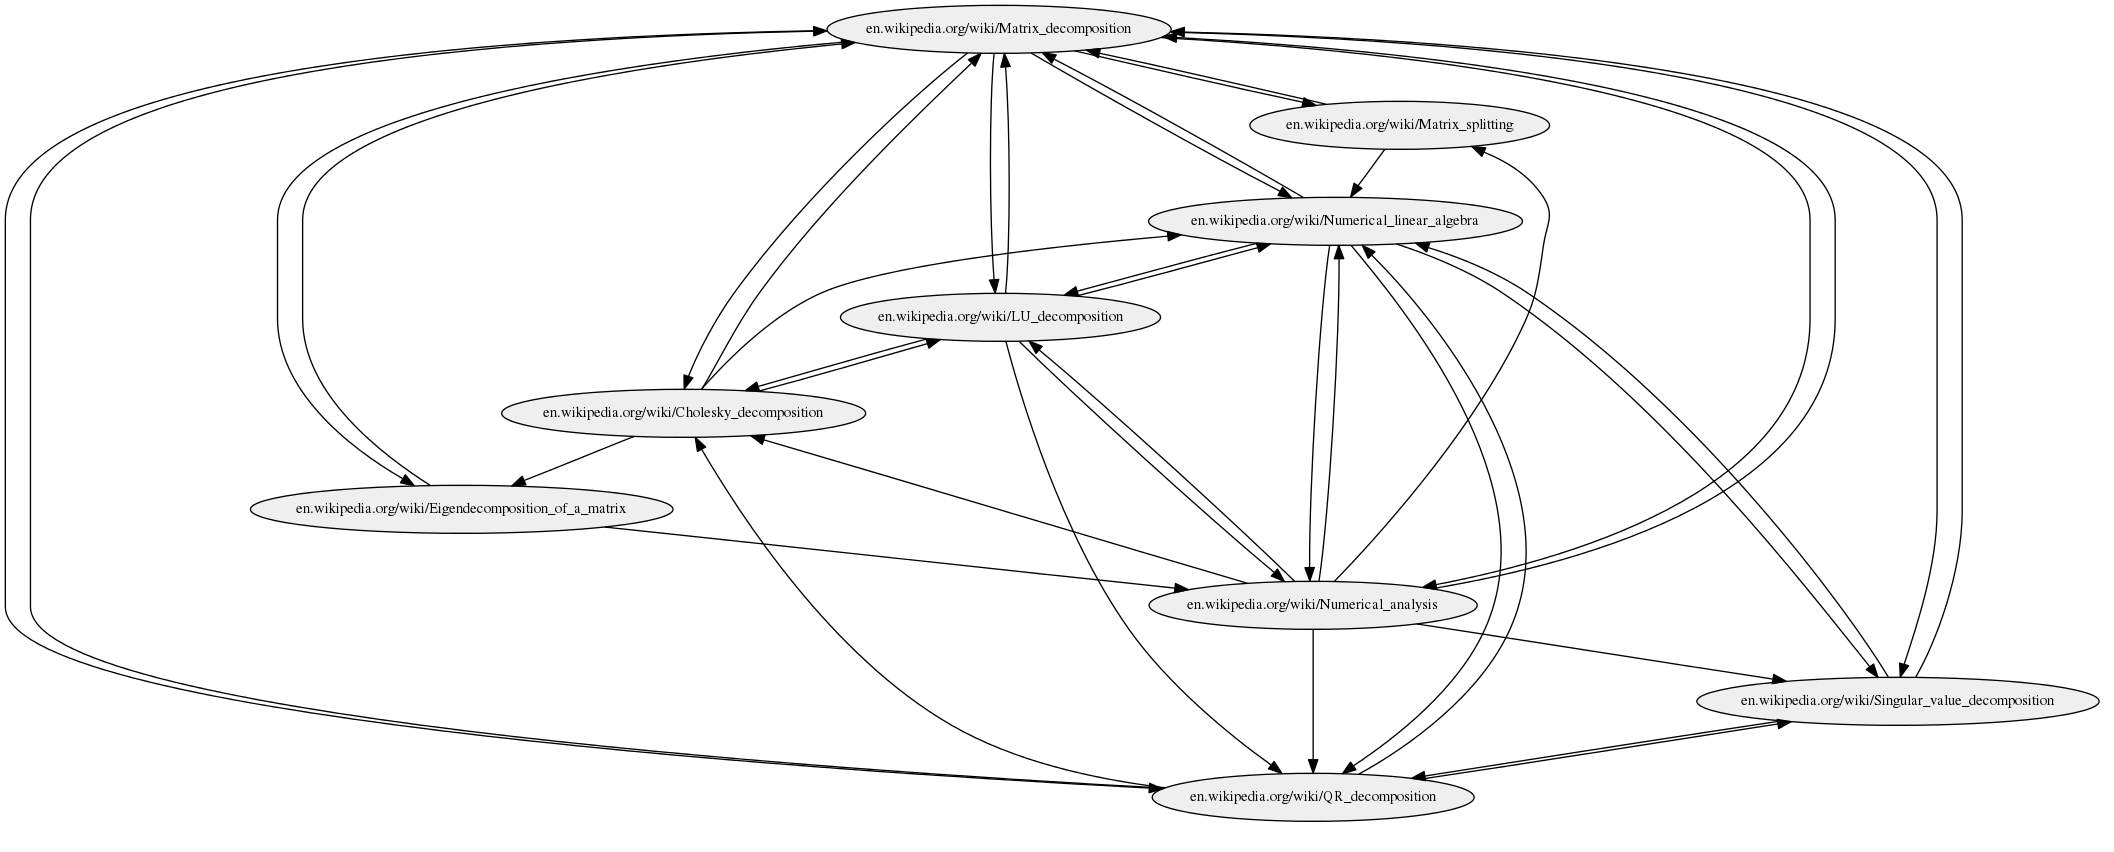
\includegraphics[width=0.75\textwidth]{exp2_conn_graph_metodos.png}
    \caption{Grafo de conectividad de p\'aginas de Wikipedia relacionadas con
        m\'etodos num\'ericos}
    \label{fig:wiki_graph}
\end{figure}

\par Sobre estas p\'aginas, calculamos los \'ordenes de PageRank e In-Deg, cuya
comparativa se encuentra detallada en el cuadro
\ref{tbl:pagerank_vs_indeg_wikipedia}. Nuevamente, In-Deg y PageRank dieron
resultados muy similares, pero no idénticos. M\'as aún, en In-Deg quedaron
varios nodos empatados, teniendo la misma cantidad de ejes entrantes. Pero esto
en PageRank no ocurri\'o, quedando definido un órden total.

\begin{table}[H]
    \centering
    \caption{\'Ordenes comparativos entre PageRank e In-Deg para Wikipedia}
    \label{tbl:pagerank_vs_indeg_wikipedia} 
    \setlength{\tabcolsep}{3pt}
    \begin{tabular}{|l|l||l|l|}
        \hline
        \multicolumn{2}{|c||}{PageRank} &\multicolumn{2}{c|}{In-Deg}\\
        \hline
        Puntaje & Nodo & Puntaje & Nodo\\
        \hline\hline
        0.196 & Matrix\_decomposition & 8 & Matrix\_decomposition\\
        0.165 & Numerical\_linear\_algebra & 7 & Numerical\_linear\_algebra\\
        0.125 & QR\_decomposition & 5 & QR\_decomposition\\
        0.106 & Numerical\_analysis & 4 & Numerical\_analysis\\
        0.105 & Singular\_value\_decomposition & 4 & LU\_decomposition\\
        0.098 & LU\_decomposition & 4 & Cholesky\_decomposition\\
        0.093 & Cholesky\_decomposition & 4 & Singular\_value\_decomposition\\
        0.057 & Eigendecomposition\_of\_a\_matrix & 2 & Eigendecomposition\_of\_a\_matrix\\
        0.050 & Matrix\_splitting & 2 & Matrix\_splitting\\
        \hline
    \end{tabular}
\end{table}

\par La diferencia entre \'ambos \'ordenes est\'a en la ubicaci\'on de
\emph{Singular value decomposition}. Mientras que en PageRank se encuentra en la
posici\'on 5, In-Deg lo lista en la 7ma ubicaci\'on. En el caso de In-Deg, la
determinaci\'on de la ubicaci\'on es determin\'istica, dependiendo del grado de
entrada del nodo que lo representa. Pero en nuestro ejemplo, vemos que existe un
empate con otros 3 nodos (como ya se ha explicado), con lo cual aqu\'i el orden
tambi\'en depende de la estabilidad y/o criterio de desempate que implemente
In-Deg. En nuestro caso, la implementaci\'on es estable, con lo cual se respeta
el orden inicial (o numeraci\'on) de los nodos. Por el otro lado, observando el
grafo podemos entender porque PageRank lo ubica en una posici\'on m\'as alta que
In-Deg: El nodo \emph{Numerical Linear Algebra}, uno de los de mayor puntaje (y
grado de entrada) tiene un link al nodo en cuesti\'on y a \emph{LU
decomposition}, pero no al resto de los valores que empatan en In-Deg. Por lo
visto en el experimento \ref{subsec:exp1}, sabemos que esto tiene un efecto de
subir el puntaje notoriamente en los nodos ''linkeados''. Luego, utilizando el
mismo razonamiento, observamos que \emph{Single value decomposition} queda por
encima de \emph{LU decomposition} por el voto/link de \emph{QR decomposition}.

\par Semánticamente, podemos observar que \textbf{en general}\footnote{\emph{QR}
queda por encima de \emph{Numerical Analysis}, creemos que esto se debe a la
morfología del grafo de referencias entre artículos en Wikipedia.} quedan
primeros en el ranking términos más \emph{generales} o \emph{abarcativos}; y a
medida que avanza el ranking se encuentran términos mas particulares.
Claramente, esta jerarqu\'ia de \emph{generalidad} es \'arbitraria para los
autores de este trabajo\footnote{¿Suma puntos hablar en tercera persona de
nosotros mismos? Very Scientific!}, aunque estimamos que habr\'a muy pocas
posibilidades de disenso al respecto para los temas representados por los nodos
del ejemplo.

\par Para evidenciar aún más la diferencia entre los algoritmos de In-Deg y
PageRank decidimos alterar expl\'icitamente el grafo de conectividad de este
\'ultimo ejemplo, agregando aristas desde los 5 nodos peor puntuados hacia uno
de los últimos en el ranking In-Deg (\emph{Eigendecomposition of a matrix}).
Esto deberia aumentar drásticamente el rankeo del ultimo elemento en In-Deg ya
que aumentamos su grado de entrada en 5, pero no tanto asi en Pagerank donde la
''calidad'' de los votantes tiene una mayor injerencia. Los resultados de este
último experimento pueden verse en el cuadro
\ref{tbl:pagerank_vs_indeg_wikipedia_modificado}. 

\begin{table}[H]
    \centering
    \caption{\'Ordenes comparativos entre PageRank e In-Deg para Wikipedia con grafo alterado explícitamente}
    \label{tbl:pagerank_vs_indeg_wikipedia_modificado}
    \setlength{\tabcolsep}{3pt}
    \begin{tabular}{|l|l||l|l|}
        \hline
        \multicolumn{2}{|c||}{PageRank} &\multicolumn{2}{c|}{In-Deg}\\
        \hline
        Puntaje & Nodo & Puntaje & Nodo\\
        \hline\hline
        0.189 & Matrix\_decomposition & 8 & Matrix\_decomposition\\
        0.137 & Numerical\_linear\_algebra & 7 & Numerical\_linear\_algebra\\
        0.123 & Numerical\_analysis & 7 & Eigendecomposition\_of\_a\_matrix\\
        0.114 & Eigendecomposition\_of\_a\_matrix & 5 & QR\_decomposition\\
        0.108 & QR\_decomposition & 4 & Numerical\_analysis\\
        0.097 & Singular\_value\_decomposition & 4 & LU\_decomposition\\
        0.089 & LU\_decomposition & 4 & Cholesky\_decomposition\\
        0.087 & Cholesky\_decomposition & 4 & Singular\_value\_decomposition\\
        0.051 & Matrix\_splitting & 2 & Matrix\_splitting\\
        \hline
    \end{tabular}
\end{table}

\par Puede observarse que respecto a In-Deg el elemento con ejes entrantes
artificiales paso a ser el
tercero por su nuevo grado de entrada aumentado. En Pagerank, el elemento subió
de ranking pero quedó por debajo de Numerical\_analysis, lo cual en principio es
raro, ya que este item quedó con puntaje 4 en In-Deg. Si miramos el grafo,
veremos que, efectivamente, el hecho de que \emph{Numerical analysis} sea apuntado por
\emph{Matrix decomposition} y \emph{Numerical linear algebra}, que son los términos mas
importantes, le da mas potencia al elemento en cuestión que al elemento
\emph{Eigendecomposition of a matrix}, apuntado por los últimos 5 de la lista.

%\par Por último, vemos que en el último experimento se acentúa el orden
%\texttt{abarcativo} de los resultados respecto al dominio de los elementos.

\medskip
\par A lo largo de este experimento pudimos evidenciar las diferencias que
existen entre dos algoritmos de elaboraci\'on de rankings distintos: In-Deg y
PageRank. Esto, que no lo hab\'iamos podido exponer en el experimento previo,
nos demostr\'o el peso que PageRank le otorga a los links provenientes de
p\'aginas web con mejores puntajes, diferenciaci\'on que In-Deg no realiza.
M\'as a\'un, nos encontramos conque In-Deg parece ser tener m\'as posibilidades
de empate en su forma de ''rankear'' que PageRank, volvi\'endose dependiente del
criterio de desempate que se utilice y convirti\'endose en otra
faceta/problema a resolver, situaci\'on que puede ser despreciada en el caso de
PageRank (las probabilidades de empate ya son chicas para pocos nodos, y las
mismas son cada vez menores a mayor cantidad). Como dato de color, observamos
que los resultados devueltos por \emph{Google} son bastante distintos de los
obtenidos con PageRank, con lo cual queda claro que a pesar de haber sido este
m\'etodo un hito en la historia del motor de b\'usqueda, el mismo ya a
evolucionado much\'isimo en pocos a\~nos, lo que demuestra la importancia del
problema estudiado. 


\newpage
\subsection{Convergencia de PageRank}
\label{subsec:exp3}
\begin{LaTeXdescription}
    \item[Objetivo] Estudiar como se comporta la convergencia en funci\'on de
        el factor de navegaci\'on $\alpha$.\\

    \item[Proposici\'on] PageRank propone una soluci\'on donde se observa a un
        conjunto de p\'aginas web como un grafo dirigido. Luego pasa este modelo
        a uno  matem\'atico, utilizando una matriz para computar una soluci\'on.
        Esta matriz, por construcci\'on, termina representando a un grafo
        completo (el grafo original no necesariamente lo era), y los valores del
        mismo dependen principalmente de 2 variables: $\epsilon$ y $\alpha$
        (algoritmo \ref{alg:power_method2}, p\'agina \pageref{alg:power_method2}
        y ecuaci\'on \ref{eq:M_def}, p\'agina \pageref{eq:M_def}). Si se observa
        el algoritmo, se ver\'a que claramente modificar el $\epsilon$ tendr\'a
        como resultado hacer que cada corrida converja en m\'as o menos
        iteraciones, ya que el criterio de parada depende de \'el. As\'i pues,
        no vemos como algo rico experimentar con este valor. En cambio, $\alpha$
        es una variable que modifica en gran medida a nuestra matriz $M$, con lo
        cual es dificil saber cual ser\'a su injerencia en la convergencia (en
        principio). El objetivo, entonces, es ver como $\alpha$ afecta al
        m\'etodo matem\'atico iterativo de la potencia en cuanto a su
        convergencia.\\

    \item[M\'etodo de Experimentaci\'on] Tomaremos 3 instancias de grafos de
        conectividad de p\'aginas web de tama\~no mediano-grande, obtenidas en
        \url{http://snap.stanford.edu/data/\#web}. Luego, correremos el
        algoritmo de PageRank para $\alpha=0.0$; $0.1$; $0.2$; $\dots$; $0.9$ y
        $\epsilon$ fijo en $0.00001$.\\

    \item[Resultados, an\'alisis y discusi\'on]
\end{LaTeXdescription}

\par En el gráfico \ref{subfig:exp3_comp} se exponen la cantidad de iteraciones
necesarias hasta converger a medida que el parámetro $\alpha$ crece. Para las 3
instancias el comportamiento observado es el mismo: a medida que el par\'ametro
$\alpha$ aumenta, la cantidad de iteraciones necesarias para converger crece
exponencialmente. Puede observarse que aunque con valores numéricos diferentes,
las curvas pertenecen a la misma familia de funciones, y por lo tanto tienen un
comportamiento id\'entico (emp\'iricamente hablando) en cuanto a la cantidad de
iteraciones en funci\'on de $\alpha$.

\begin{figure}[H]
    \centering
    \caption{An\'alisis de Convergencia en funci\'on de $\alpha$}
    \subfloat[][Iteraciones hasta Converger en funci\'on de $\alpha$]{
        \label{subfig:exp3_comp}
        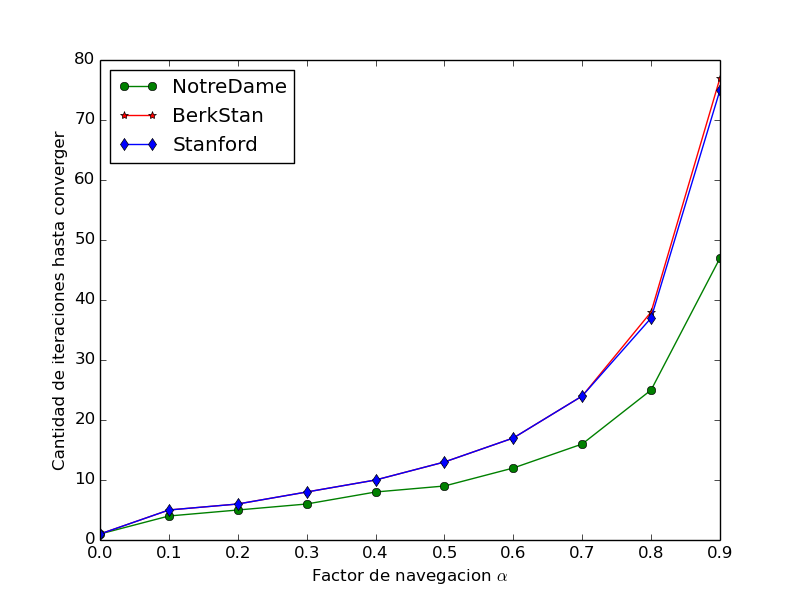
\includegraphics[width=.5\textwidth]{exp3_iteraciones_funcion_alpha.png}
    }
    \subfloat[][Velocidad de convergencia en funci\'on de $\alpha$\\Escala
    logar\'itmica]{
        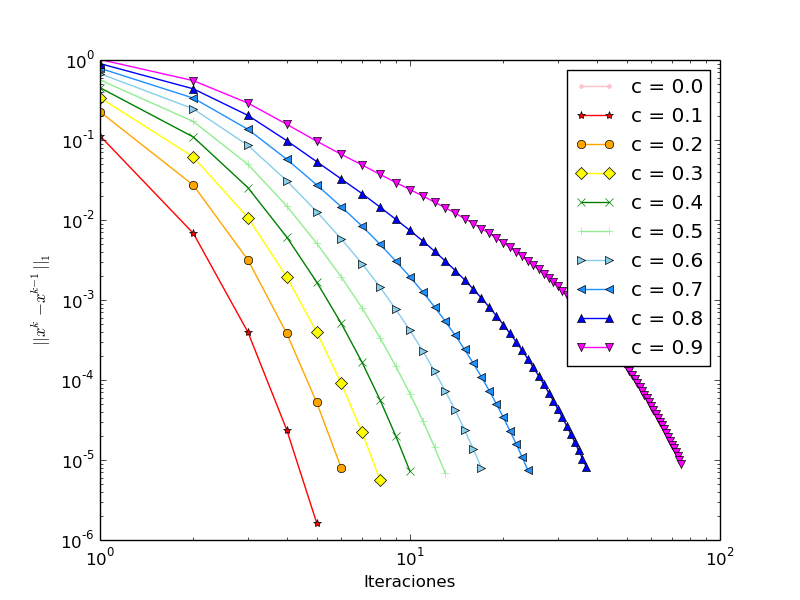
\includegraphics[width=.5\textwidth]{exp3_diff_funcion_iteraciones_standford.png}
        \label{subfig:exp3_diff}
    }
\end{figure}

\par Como se explic\'o en la secci\'on \ref{sec:introduccion}, el factor
$\alpha$ hace variar la proporci\'on entre $S$ y la matriz equiprobable a la
hora de definir a $M$. Es decir, en el rango de posibles valores de $\alpha$, la
\'unica manera en la que se afecta a $M$ es en los valores de cada uno de sus
elementos. Pero para ning\'un $\alpha$ se puede pasar a tener un elemento nulo
en $M$ (justamente se quer\'ia tener la representaci\'on de un digrafo
completo). As\'i pues, la pregunta pasa a ser: ¿Por qu\'e a mayor $\alpha$ se
necesitan m\'as iteraciones para converger?

\par Se nos ocurre que, volviendo al contexto de una cadena de Markov y el
navegante aleatorio, un $\alpha$ peque\~no nos genera una matriz de transici\'on
''m\'as'' equiprobable (recordar la definici\'on de $M$ en la ecuaci\'on
\ref{eq:M_def}, p\'agina \pageref{eq:M_def}) y dado que el método de la potencia
comienza inicialmente con el vector equiprobable, le toma pocas iteraciones
converger. A medida que $\alpha$ aumenta, el grafo generado denota más la
navegación estricta por los links entre los sitios, reduciendo la probabilidad
de teletransportación. Es decir, a mayor $\alpha$, el grafo se ''parece m\'as''
al grafo de conectividad original no adulterado (con los dangling nodes ya
resueltos), en el sentido de que $S$ predomina mucho m\'as en $M$ que
$(\rfrac{1}{n})ee^T$. Esta matriz $S$ no necesariamente representa un grafo
fuertemente conexo, una de las condiciones necesarias para asegurar convergencia
del método de la potencia en el contexto de este problema, con lo cual el método
de la potencia inicia sus iteraciones con una, si se quiere, \textbf{seguridad
de convergencia más débil}.

\par Respecto a la velocidad de convergencia, exponemos los resultados de una
sola instancia ya que para las 3 instancias los resultados son similares. Como
puede observarse en el gráfico \ref{subfig:exp3_diff}, a medida que el factor de
navegacion $\alpha$ crece, la velocidad de convergencia disminuye,
obteni\'endose curvas cada vez m\'as pronunciadas.

\par La ''velocidad de convergencia'' la definimos como la distancia
\emph{Manhattan} entre los autovectores $\vec{x^{(k)}}$ y $\vec{x^{(k-1)}}$
calculados en dos iteraciones consecutivas. Mientras mayor sea la distancia,
m\'as r\'apido decimos que se converge\footnote{Asumiendo que $\vec{x^{(k)}} <
\vec{x^{(k-1)}}$, caso contrario nos estar\'iamos alejando del criterio de corte
del m\'etodo, es decir, de converger.}, pues se est\'a acerc\'andose cada vez
\textbf{m\'as rápido} al umbral de corte del algoritmo (basado en $\epsilon$ o
una cantidad fija m\'axima de iteraciones\footnote{Esto se implementa, ya que si
bien la teor\'ia nos indica que el m\'etodo convergir\'a, los errores
n\'umericos de la aritm\'etica finita puede hacer que esto no ocurra.}).

\par Nuestra explicaci\'on para este comportamiento es exactamente la misma que
se expuso para el caso de las iteraciones hasta converger en funci\'on de
$\alpha$. Sin ir m\'as lejos, estamos hablando del mismo fen\'omeno, salvo que
en el caso de la figura \ref{subfig:exp3_diff} hacemos hincapi\'e en
\textbf{como} se acerca el m\'etodo al vector soluci\'on, mientras que en la figura
\ref{subfig:exp3_comp} observamos m\'as en detalle la \textbf{cantidad de
iteraciones} que se necesitan. Sin embargo, ambos gr\'aficos nos muestran lo
mismo: \textit{a que velocidad}, o \textit{cuanto tiempo/iteraciones} se
requieren para converger en funci\'on de $\alpha$.

\par Ahora bien, hemos visto como $\alpha$ afecta a la convergencia. S\'i esto
fuera lo \'unico, claramente siempre elegir\'iamos el valor que nos permita
converger m\'as r\'apido. Ocurre que, como vimos en el experimento
\ref{subsec:exp1}, el $\alpha$ afecta al orden obtenido tambi\'en, es decir, a
la calidad del resultado. As\'i pues, la elecci\'on de este par\'ametro ser\'a
la b\'usqueda del equilibrio \emph{efectividad} y \emph{eficiencia}, u entre
calidad del resultado y ti\'empo de c\'omputo (intuitivamente, m\'as iteraciones
implican mayor tiempo de c\'omputo). La bibliograf\'ia consultada nos indica que
en su momento, Google fij\'o inicialmente este par\'ametro en $0.85$,
considerando a este un \emph{trade-off} lo suficientemente
bueno\cite{Bryan2006}\cite{Langville2006}.

\par As\'i pues conclu\'imos nuestra experimentaci\'on sobre la convergencia del
m\'etodo de la potencia para PageRank. Llegamos a un resultado inmediato que nos
dice que a mayor $\alpha$ tendremos una velocidad de convergencia menor y, ergo,
una cantidad de iteraciones necesaria mayor para obtener un resultado lo
suficientemente apr\'oximado. Tambi\'en evaluamos brevemente la contracara de
tener un tiempo de convergencia chico: el resultado obtenido no necesariamente
es el mismo ya que predomina m\'as la equiprobabilidad de los ejes de
teletransportaci\'on artificalmente a\~nadidos a la matr\'iz $M$. Tambi\'en
obtuvimos como resultado que este comportamiento es, presumiblemente (har\'ia un
falta un an\'alisis m\'as minucioso para poder afirmarlo), el mismo para
cualquier instancia de entrada, m\'as all\'a de que la cantidad de iteraciones
absoluta entre dos instancias pueda variar para el mismo $\alpha$, el
comportamiento en funci\'on de $\alpha$ parecer\'ia ser el mismo.


\newpage
\subsection{An\'alisis de Tiempo de C\'omputo}
\label{subsec:exp4}
\begin{LaTeXdescription}
    \item[Objetivo] Analizar la complejidad temporal del m\'etodo.\\

    \item[Hip\'otesis] Proponemos que el tiempo de c\'omputo por iteraci\'on
        para una instancia y $\epsilon$ fijos ser\'a siempre el mismo para todo
        $\alpha$. Tambi\'en proponemos que el tiempo de c\'omputo por interación
        para $\epsilon$ fijo ser\'a el mismo para \textbf{toda instancia} (sin
        importar tama\~no, cantidad de ejes, etc).\\

    \item[Proposici\'on] De los experimentos previo hemos llegado a la
        conclusi\'on de que a mayor $\alpha$, mayor cantidad de iteraciones
        ser\'an necesarias para converger, lo cual implica inmediatamente un
        mayor tiempo de c\'omputo requerido. La pregunta ideal a responder
        ser\'ia ''cu\'anto tiempo'', pero tambi\'en concluimos previamente que
        la cantidad de iteraciones es dependiente (entre otros factores) de la
        instancia de entrada. Con lo cual, responder a esta pregunta en el
        contexto de este trabajo es imposible sin una cota te\'orica para la
        cantidad de iteraciones (que ni siquiera sabemos si existe). En cambio,
        lo que s\'i podemos analizar es si el tiempo de c\'omputo \textbf{por
        iteraci\'on} es el mismo para toda instancia, sin importar el
        $\epsilon$\footnote{M\'as all\'a de para nuestros experimentos lo
        estemos dejando fijo.} o $\alpha$. Analizamos entonces si el tiempo por
        iteraci\'on var\'ia seg\'un la densidad de la instancia inicial, y a su
        vez si varía para distintos valores de $\alpha$.\\

    \item[M\'etodo de Experimentaci\'on] Tomamos 3 instancias de tama\~no
        mediano-grande, con una diferencia relativa de densidad entre ellas
        significativa. Particularmente, tomamos las mismas del experimento
        anterior. Luego resolvemos cada instancia con PageRank 10 veces para
        $\alpha=0.0$; $0.1$; $0.2$; $\dots$; $0.9$\footnote{Totalizando un total
        de 300 corridas del m\'etodo (10 corridas para 10 valores de $\alpha$
        para 3 instancias distintas).}. Tomamos entonces para cada instancia y
        $\alpha$ fijos, el promedio de los tiempos de c\'omputo. Por \'ultimo,
        calculamos el tiempo de c\'omputo por iteraci\'on dividiendo este
        promedio por la cantidad de iteraciones totales que necesit\'o el
        m\'etodo para converger.\\

    \item[Resultados, an\'alisis y discusi\'on]
\end{LaTeXdescription}

\par Consideramos 2 enfoques para extraer conclusiones, el primero analiza el
tiempo consumido por iteración por el método de la potencia para diferentes
valores de $\alpha$ y el segundo se centra en el tiempo por iteraci\'on respecto
de la densidad de la instancia/grafo de entrada\footnote{Al referirnos a
\emph{densidad} de un grafo, nos referimos a la cantidad de ejes que tiene. A
mayor cantidad de ejes, m\'as denso es.}.

\begin{figure}[H]
    \centering
    \caption{An\'alisis de Tiempo de C\'omputo} %en funci\'on de $\alpha$}
    \subfloat[][Tiempo por Iteraci\'on en funci\'on de $\alpha$.]{
        \label{subfig:exp4_tiempo_iteracion}
        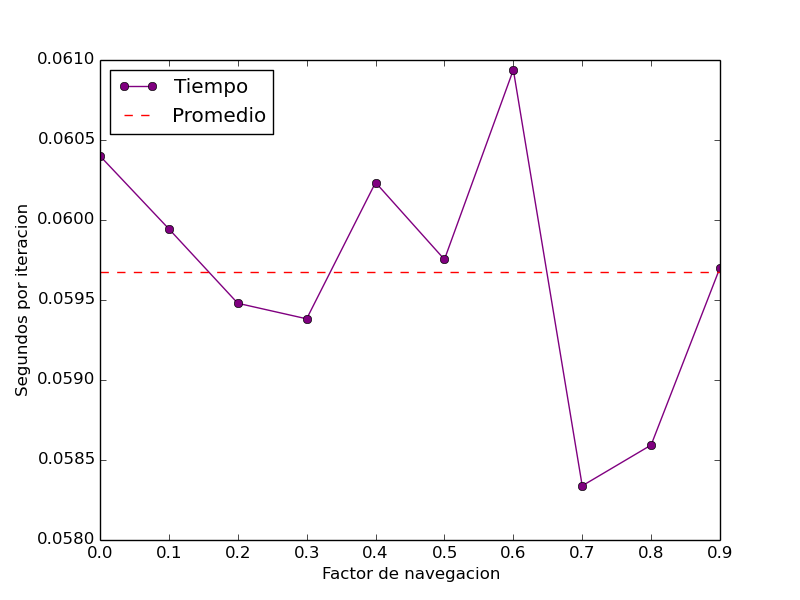
\includegraphics[width=.55\textwidth]{exp4_tiempo_por_iteracion_notredame.png}
    }
    %\begin{figure}[H]
    %    \centering
        \subfloat[][Tiempo por Iteraci\'on promedio vs Densidad del Grafo]{
            \label{subfig:exp4_den}
            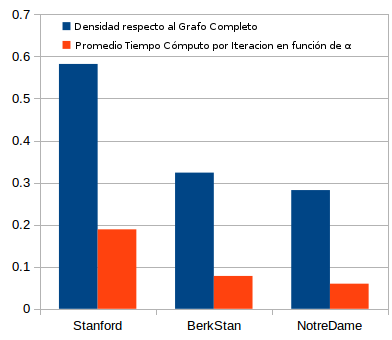
\includegraphics[width=.45\textwidth]{exp4_tiempo_vs_densidad.png}
        }
        %\caption{An\'alisis de Tiempo de C\'omputo en funci\'on de la densidad del Grafo}
    %\end{figure}
    %\subfloat[][Tiempo por Iteraci\'on en funci\'on de $\alpha$. Escala logarítmica]{
    %    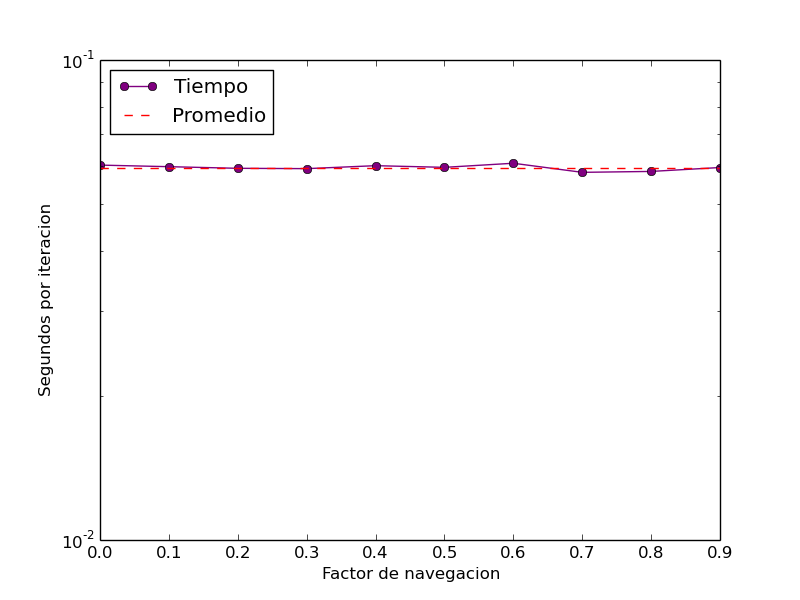
\includegraphics[width=.45\textwidth]{exp4_tiempo_por_iteracion_notredame_log.png}
    %    \label{subfig:exp4_tiempo_iteracion_log}
    %}
\end{figure}

\par Para el primer enfoque, observemos los resultados obtenidos en la figura
\ref{subfig:exp4_tiempo_iteracion}. En el mismo observamos dos curvas. La
primera, \emph{Tiempo}, que representa el tiempo por iteraci\'on promedio para
cada $\alpha$ (calculado como el tiempo promedio hasta converger de las 10
ejecuciones para un $\alpha$ fijo, dividido por la cantidad de iteraciones que
necesit\'o); y la segunda \emph{Promedio} que no es otra cosa que el promedio de
los tiempos por iteraci\'on calculados para la curva \emph{Tiempo}. Los
resultados expuestos en esta figura son similares para las 3 instancias de
prueba que se tomaron, con lo cual se decidi\'o exponer una sola.

\par Puede observarse en esta misma figura que el tiempo por iteraci\'on
calculado en funci\'on de $\alpha$ oscila en valores muy pequeños alrededor del
promedio. Para ilustrar esto, presentamos en el cuadro
\ref{tbl:exp4_data_notredame} las m\'etricas empíricas del experimento.

\begin{table}[H]
    \centering
    \caption{Métricas del tiempo por iteracion respecto de $\alpha$}
    \label{tbl:exp4_data_notredame} 
    \setlength{\tabcolsep}{3pt}
    \begin{tabular}{|l|l|}
        \hline
        Métrica & Segs\\
        \hline\hline
        Promedio & 0.059676\\
        Desv\'io Est\'andar & 0.000788\\
        M\'inimo & 0.058338\\
        M\'aximo & 0.060938\\
        Diferencia \%\footnotemark& 4.266231\\
        \hline
    \end{tabular}
\end{table}
\footnotetext{Diferencia \%: 100*(max-min)/max.}


\par Estas variaciones seguramente se deben al \emph{scheduler} del sistema
operativo y a fenómenos de bajo nivel de las corridas de los
experimentos. De hecho, ya vimos en el experimento \ref{subsec:exp3} que a
medida que aumentamos el $\alpha$, m\'as iteraciones ser\'an necesarias para
converger. Obviamente esto implica un mayor tiempo de c\'omputo, ergo, la
ejecuci\'on del experimento se vuelve a\'un m\'as sensible pues al estar m\'as
tiempo ejecut\'andose m\'as probabilidades hay de que el Sistema Operativo
decida darle el CPU a otro proceso de mayor prioridad que surja (o que al estar
tanto tiempo ejecut\'andose, su prioridad vaya bajando).

\par Finalmente conclu\'imos que que el tiempo por iteraci\'on es constante, ya
que en las m\'etricas nos confirman, al observar los valores muy peque\~nos del
desv\'io est\'andard y diferencia porcentual, que estas diferencias para
distintos $\alpha$ sean muy probablemente errores de medici\'on (recordemos que
adem\'as estamos trabajando con instancias de entrada de tama\~no
mediano-grande).

\par Habiendo llegado a la conclusi\'on que la hip\'otesis sobre el tiempo de
c\'omputo por iteraci\'on es constante, debemos analizar por qu\'e. Repasando la
secci\'on \ref{sec:implementacion}, podemos decir que es razonable el
comportamiento presupuesto y observado, ya que el valor de $\alpha$ no modifica
la \emph{densidad} de la matriz original de conectividad $A$. Recordemos
entonces que nuestra implementaci\'on se basa en el algoritmo
\ref{alg:power_method3}, p\'agina \pageref{alg:power_method3}, que multiplica
usando justamente esta matriz $A$ y aprovechando que la misma es esparsa. Al no
modificar esta caracter\'istica la selecci\'on del par\'ametro $\alpha$, podemos
afirmar que la cantidad de $flops$ necesarios para el producto matriz-vector se
mantendr\'a constante en funci\'on de $\alpha$ (de hecho, $\alpha$ es un
par\'ametro que luego multiplica al vector resultante $A\vec{x}^{(k-1)}$ en
nuestro algoritmo, con lo cual no afecta en lo absoluto al producto
matriz-vector que involucra a $A$).

\par El segundo enfoque centra su atención en el tiempo por
iteracion respecto a la densidad del grafo asociado a la instancia de entrada.
Al contrario que lo esperado, la densidad (cantidad de ejes) del
grafo \textbf{s\'i} altera el tiempo de cómputo por iteración. Si observamos la
figura \ref{subfig:exp4_den}, observaremos que a mayor densidad, mayor tiempo
por iteraci\'on se necesita.

\par En esta figura se compara el tiempo promedio consumido\footnote{Se utiliza
el valor promedio del tiempo para todos los factores de navegación.} contra una
medida de densidad del grafo\footnote{Se toma como métrica un cociente entre la
cantidad de aristas del gráfo y la cantidad de aristas de una \emph{clique} de
su misma cantidad de nodos; multiplicado por una constante para igualar las
magnitudes con los valores de los tiempos de c\'omputo.}, y se v\'e, para las 3
instancias evaluadas, que el crecimiento del tiempo de c\'omputo parecer\'ia ser
l\'ineal en funci\'onde la densidad del grafo. Dado que s\'olo experimentamos
con estas 3 instancias, ser\'ia muy abrupto hacer dicha afirmaci\'on, pero si
podemos decir que tenemos sospechas de que eso ocurra, dejando este aspecto para
un futuro posible experimento\footnote{Vale la pena aclarar, en este caso, que
podr\'iamos considerar a nuestras 3 instancias como poco densas, m\'as alla de
la diferencia notoria de densidad entre ellas.}.

\par Volviendo al hecho de que a mayor densidad, mayor ti\'empo de c\'omputo,
llegamos a la conclusi\'on de que esto se debe al mismo motivo que en el primer
enfoque, salvo que esta vez justifica el hecho de que \textbf{s\'i} se requiera
m\'as tiempo de c\'omputo. Ocurre que al ser la instancia de entrada m\'as
densa, menos esparsa ser\'a $A$ (m\'as ejes implica mayor cantidad de valores no
nulos en la matriz), y por lo tanto el producto $A\vec{x}$ de la
implementaci\'on del m\'etodo efectuar\'a m\'as $flops$.

\medskip
\par Finalizando, concluimos que 1 de nuestras hip\'otesis era correcta, y la
otra no. Peculiar es, que las justificaciones que le encontramos a ambos
comportamientos (la relaci\'on tiempo de c\'omputo por iteraci\'on en funci\'on
de $\alpha$ y de la densidad de la instancia) es la misma: mientras que $\alpha$
no afecta a la densidad de la matriz de conectividad pesada $A$, cosa que si lo
hace la cantidad de ejes del grafo. Es decir, terminamos entendiendo que el
principal aspecto a tener en cuenta a la hora de ver como se ver\'a afectado el
tiempo de computo (para nuestra implementaci\'on basada en el algoritmo
propuesto por Kamvar et al.\cite{Kamvar2003}) ser\'a la
densidad/esparcidad\footnote{Coloquialismo.} de la matriz inicial del modelo.


\newpage
\subsubsection{PageRank/GeM vs Orden Total Conocido}
\label{subsec:exp5}
\begin{LaTeXdescription}
    \item[Objetivo] Analizar la convergencia del modelo GeM asumiendo que
        existe ranking ideal y correcto al cual converger.\\

    \item[Hip\'otesis] PageRank, utilizando el modelo GeM, converge finalmente a
        un ''Orden Real'' o ''Correcto'' de los competidores deportivos, si este existe.
        Adem\'as, no necesitar\'a de un grafo completo (los resultados de todos
        contra todos) para converger al mismo.\\

    \item[Proposici\'on] Como se coment\'o previamente en la experimentaci\'on
        sobre p\'aginas web, establecer cuál es el ''mejor orden'' u ''orden
        correcto'' es completamente arbitrario. No hay una vara sobre la cual
        medir. En los deportes esto es a\'un más evidente, ya que depende de
        los resultados deportivos, ¿y qui\'en es capaz de afirmar que la
        probabilidad de que Platense -el mejor equipo del mundo e insipirador
        del t\'itulo del enunciado de este trabajo- le gane al Barcelona es $0$?
        As\'i pues, en el caso de los deportes tampoco tenemos un orden total,
        conocido y determin\'istico para verificar que el resultado de PageRank
        es el correcto. Pero si existiese este orden, si fuese determin\'istico,
        ¿PageRank convergir\'ia al mismo?\\

    \item[M\'etodo de Experimentaci\'on] Generamos dos instancias ideales y
        completamente abstractas de los resultados de un torneo de f\'utbol con
        10 y 50 equipos respectivamente, que juegan todos contra todos una
        \'unica vez (45 partidos para la primera instancia, 1225 para la
        segunda). Las instancias son construidas de manera tal que $equipo_i$ le
        gana a $equipo_j$ si y s\'olo si $i<j$. Es decir, el ranking correcto es
        la numeraci\'on de los equipos de forma ascendente, y cada $equipo_i$
        ocupa el puesto $i$.

        \par Aprovechamos el hecho de que en los deportes hay una componente
        temporal y generamos los partidos por fecha (es decir, grupos de
        partidos que ocurren todos al mismo tiempo, o al menos as\'i ser\'a para
        la perspectiva del algoritmo, que recibir\'a todos los partidos de una
        fecha juntos). En cada fecha se enfrentan, de a dos, equipos que no se
        hayan enfrentado todav\'ia y que no jueguen otro partido esa misma
        fecha. Dentro de esas restricciones, los enfrentamientos de cada fecha
        se eligen al azar, pero con una semilla fija (5) para obtener
        reproducibilidad en los experimentos. \textbf{Notar que la cantidad de
        fechas necesarias para que se jueguen todos los partidos no est\'a
        determinada \'unicamente por la cantidad de equipos sino que depende
        tambi\'en de como se elijan los enfrentamientos de cada fecha. Esto se
        debe a que confeccionar un generador de instancias aleatorias que
        respete las restricciones y genere un fixture de $n-1$ equipos es
        complejo y escapa a los objetivos de este trabajo. As\'i pues, nuestra
        instancia de 10 equipos \underline{consta de 11 fechas} y la instancia
        de 50 equipos \underline{consta de 53 fechas}}.

        \par El resultado de todos los partidos es siempre 1 a 0. No hace falta
        considerar empates dado que siempre hay un ganador.
        
        \par Ejecutamos
        GeM tantas veces como fechas haya, pas\'andole en cada instancia una
        fecha m\'as. Es decir, en la ejecuci\'on 1 le pasamos los resultados de
        la fecha 1, en la 2 los resultados de la fecha 1 y 2, y as\'i
        sucesivamente. Para cada resultado de GeM, comparamos el ranking
        obtenido con el correcto, para alguna medida de distancia entre
        rankings, que definiremos m\'as adelante.

        \par Hace falta considerar un detalle importante, que es qu\'e
        decisi\'on tomar ante empates del ''puntaje'' asignado por GeM. Si
        desempat\'aramos por n\'umero de equipo de manera ascendente caer\'iamos
        en el molesto caso de que ya desde antes de empezar el torneo la salida
        de GeM coincidir\'ia con el orden ideal. Lo mismo vale para cualquier
        subconjunto de competidores empatados en un momento dado: su orden
        relativo coincidir\'ia con el ideal, aunque por casualidad y no por
        virtud del algoritmo. Resolvimos entonces ''romper'' el caso y que el
        desempate se realice de manera descendente, asegur\'andonos as\'i de no
        evaluar como correctos resultados en donde hay muchos empates.

        \par Repetimos el experimento variando los valores de $\alpha$ en
        factores de $0.2$, para estudiar la convergencia en cada caso.  De
        confirmarse nuestra hip\'otesis la diferencia/distancia del ranking
        respecto del orden total ideal (que sabemos que existe por
        construcci\'on) deber\'ia llegar a ser 0, eventualmente ''antes'' de que
        se hayan jugado todas las fechas.\\

    \item[Resultados, an\'alisis y discusi\'on]
\end{LaTeXdescription}

\par En primer lugar, como hemos adelantado, debemos decidir cómo determinar la
''distancia'' entre dos rankings. Es decir, determinar alguna manera de comparar
dos rankings dados, y poder tener una magnitud de cuan parecidos son. Para ello
consideramos algunas opciones dados dos rankings A y B, de entre las cuales
mencionamos:

\begin{enumerate}
        \item La sumatoria de la distancia, para cada competidor, entre su
            posici\'on en el ranking A y la posici\'on en el ranking
            B.\label{itm:distancia_rankings}
        \item La cantidad de competidores que aparecen, en A, en una posición distinta a la que aparecen en B.
        \item La sumatoria, para cada competidor, de la cantidad de equipos que tiene por encima en A y que tiene por debajo en B.
\end{enumerate}

\par Luego de evaluar estas opciones (y algunas m\'as no tan concisas),
decidimos trabajar de aqu\'i en m\'as con la distancia basada en la suma de las
distancias de todos los competidores (definici\'on de distancia n\'umero
\ref{itm:distancia_rankings}). Consideramos que dicha forma de tomar la
distancia entre dos rankings, de alguna manera nos est\'a se\~nalando cuántas
permutaciones de elementos/equipos contiguos hay entre un ranking y el otro,
cosa que no queda tan claro con las dem\'as opciones. Y esa forma de medir la
distancia es la que consideramos que se ajusta a lo que queremos observar del
dominio del problema: cu\'antos equipos est\'an ubicados distinto y cuán lejos.

\begin{figure}[H]
    \caption{Distancia al orden total ideal/correcto ($c = \alpha$)}
    \label{fig:exp5_1}
    \centering
    \subfloat[][Torneo de 10 equipos]{
        \label{subfig:exp5_10equipos}
        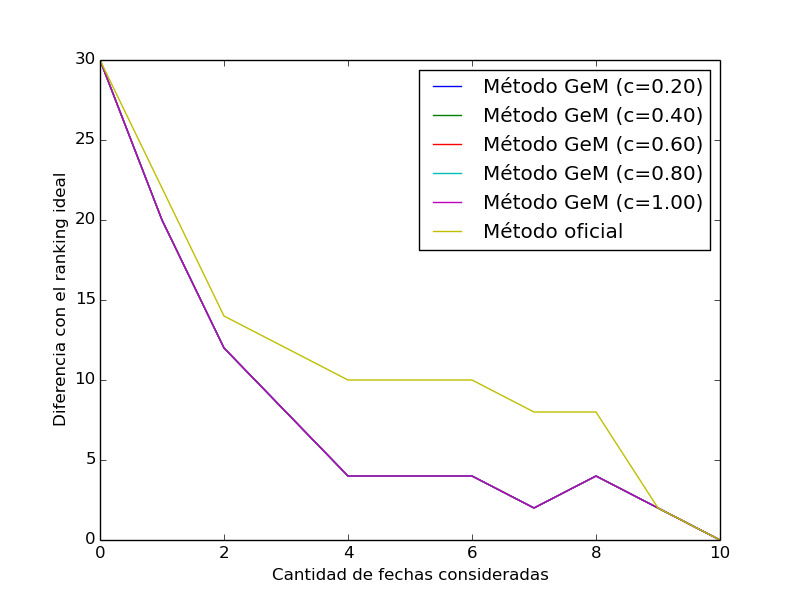
\includegraphics[width=.5\textwidth]{exp5_10_equipos.png}
    }
    \subfloat[][Torneo de 50 equipos]{
        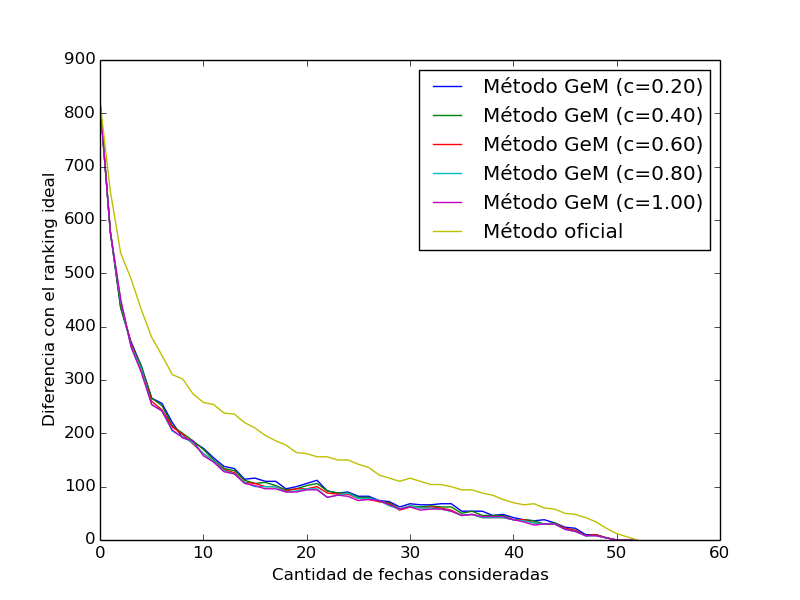
\includegraphics[width=.5\textwidth]{exp5_50_equipos.png}
        \label{subfig:exp5_50equipos}
    }
\end{figure}

\par La hip\'otesis fue confirmada. GeM converge al Orden Real para todos los
valores no nulos de $\alpha$ y no precisa todas las fechas para hacerlo, como se
puede observar en la figura \ref{fig:exp5_1}. Sin embargo, necesita una cantidad
significativa: para todos los valores no nulos de $\alpha$ fueron necesarias 10
de 11 fechas para el caso de 10 equipos y 50 de 53 fechas para el caso de 50
equipos.

\par El caso $\alpha=0$ no funciona porque la matriz termina descartando los
resultados de los equipos y usando simplemente la misma probabilidad para
cualquier equipo. En adelante dejaremos de lado este caso.

\par La variaci\'on $\alpha$ en el caso de 10 equipos no represent\'o
diferencias en el orden devuelto en cada fecha. es por eso que en la figura
\ref{subfig:exp5_10equipos} no se ven m\'as que dos curvas (una de las cuales
corresponde al siguiente experimento): estan todas superpuestas. En el caso de
50 equipos s\'i hubo leves diferencias en el orden devuelto en cada fecha.
Observamos que a mayor $\alpha$ el algoritmo en general converge ''mejor'' al
Orden Real (es decir, dada la misma cantidad de fechas, se acerca m\'as), aunque
siempre precisa 50 fechas para converger al orden real (figura
\ref{subfig:exp5_50equipos}). La diferencia de todos modos es peque\~na y probablemente se deba a que, en
nuestro modelo ideal, las victorias son totalmente transitivas: la probabilidad
de que $C$ le gane a $A$ dado que $A$ le gan\'o a $B$ y $B$ le ganó a $C$ es
siempre $0$.  Como valores peque\~nos de $\alpha$ tienden a agregar una
probabilidad de que $C$ efectivamente le gane a $A$, la convergencia mejora
levemente para valores altos de $\alpha$ (donde esa probabilidad artificial es
cada vez menor). Sin embargo, variando la semilla usada para ordenar los
enfrentamientos encontramos casos en donde un valor mayor de $\alpha$ empeoraba
la convergencia en alg\'un punto (ver figura \ref{subfig:exp5_c_malo}), por lo
que no podemos generalizar esta conclusi\'on.

\par As\'i pues, motivados por estos resultados, realizamos la siguiente
experimentaci\'on.

%---------------------------------------------------------------
\subsubsection*{PageRank vs Ranking FIFA en un caso de Orden Total Conocido}
\label{subsec:exp5_aux}
\begin{LaTeXdescription}
    \item[Objetivo] Comparar GeM contra el raking est\'andar del f\'utbol en un
        caso ideal.\\

    \item[Hip\'otesis] PageRank, utilizando el modelo GeM, converge m\'as
        r\'apido al ''Orden Real'', si lo hay, que el sistema oficial del
        f\'utbol asociado establecido por la FIFA\cite{fifa}.\\

    \item[Proposici\'on] Asumiendo que se confirm\'o la hip\'otesis del
        experimento anterior, nos interesa analizar si, asumiendo que existe un
        orden ideal/correcto, GeM se comporta peor, igual o mejor que la forma
        est\'andar de ordenar a los equipos (por puntos, 3/1/0 puntos para
        victoria/empate/derrota) donde ''comportarse'' mejor significa que con
        la misma información disponible (por ejemplo, la mitad de los partidos
        jugados) se acerca m\'as al orden ideal.\\

    \item[M\'etodo de Experimentaci\'on] Consideramos las mismas instancias de
        prueba que el experimento anterior. Comparamos la distancia entre GeM y
        el orden ideal contra la distancia entre el ordenamiento est\'andar y el
        orden ideal, usando la misma definici\'on de distancia de rankings que
        para el experimento anterior y el mismo criterio para ordenar equipos
        empatados en puntaje. De confirmarse nuestra hip\'otesis, deber\'iamos
        ver que GeM se acerca ''m\'as r\'apido'', es decir, con menos fechas, al
        orden ideal.\\

    \item[Resultados, an\'alisis y discusi\'on] 
\end{LaTeXdescription}

\begin{figure}[H]
    \caption{Casos Patol\'ogicos (10 equipos, $c = \alpha$)}
    \label{fig:exp5_2}
    \centering
    \subfloat[][Caso particular malo para $\alpha$ grande]{
        \label{subfig:exp5_c_malo}
        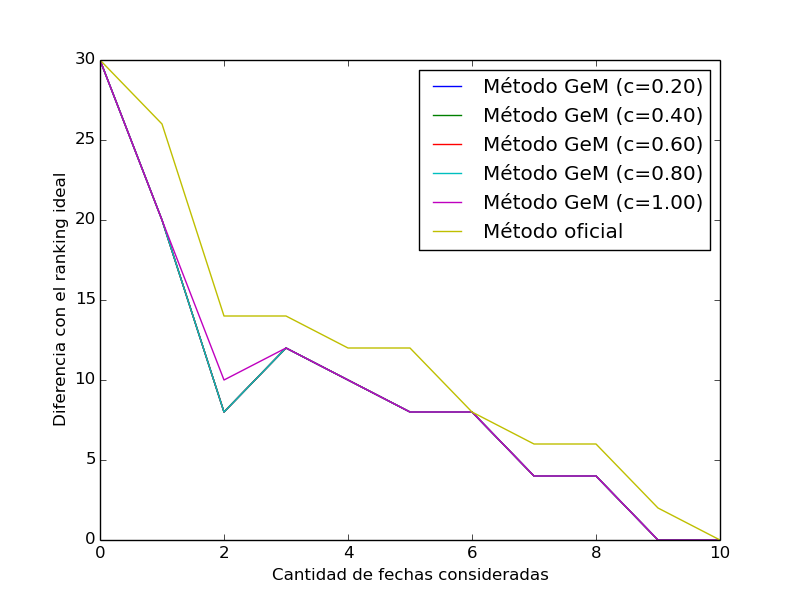
\includegraphics[width=.5\textwidth]{exp5_ejemplo_c_malo.png}
    }
    \subfloat[][Caso particular malo para GeM]{
        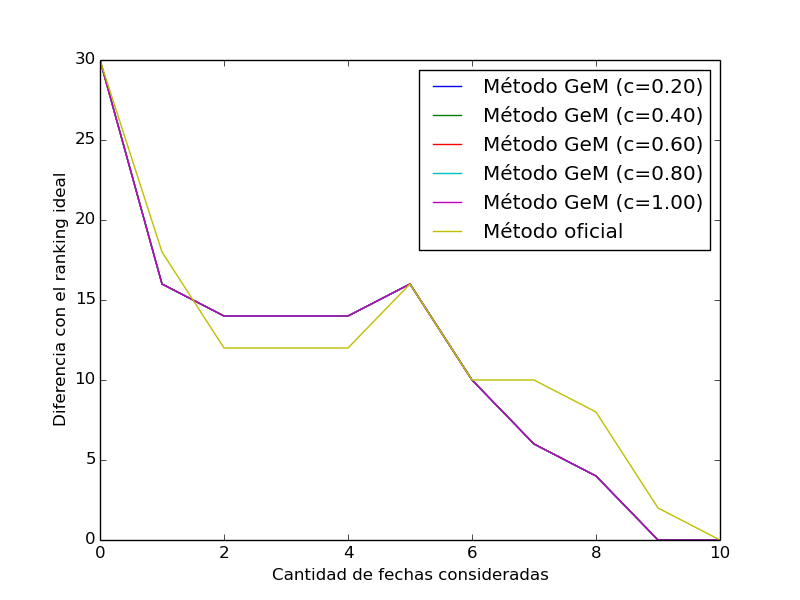
\includegraphics[width=.5\textwidth]{exp5_ejemplo_gem_malo.png}
        \label{subfig:exp5_gem_malo}
    }
\end{figure}

\par Comparamos GeM con el orden oficial, establecido por asignación de puntos
(3-1-0) y confirmamos tambi\'en nuestra hip\'otesis de que en el caso promedio,
GeM se comporta mejor que el orden oficial de asignaci\'on de puntajes,
acerc\'andose más al ideal para cualquier cantidad de fechas.

\par Sin embargo tambi\'en encontramos semillas para las cuales esto no era real
en alg\'un punto (ver figura \ref{subfig:exp5_gem_malo}) por lo que tampoco
podemos generalizar esta conclusi\'on.

\par Por \'ultimo, dado que los dos casos ''patol\'ogicos'' fueron encontrados
con la instancia de pocos equipos (10) y no logramos encontrar una semilla que
los genere en el caso de muchos (50), podr\'iamos argumentar que GeM se comporta
''mejor'' cuando la cantidad de equipos es grande. Queda fuera de los alcances
de este trabajo confirmar m\'as sistem\'aticamente esa hip\'otesis, pero es un
buen trabajo futuro.

%---------------------------------------------------------------
\medskip
\par En este experimento se trabaj\'o principalmente con instancias artificiales
''de juguete''. Las mismas lejos est\'an de representar la realidad, pero nos
sirvieron para poder asegurar que el modelo GeM ''descubrir\'ia'' el ranking
justo (o real, como dir\'ia Platon) si este existiese. A\'un as\'i, observamos
que para llegar a este ranking el modelo requerir\'a de mucha informaci\'on de
entrada, lo cual le quita quiz\'as utilidad como predictor de resultados de
torneos\footnote{Sin \'animo de menospreciar a GeM, si uno tiene los datos de 50
sobre 53 fechas, predecir con buena probabilidad de acierto el orden final no es
necesariamente una tarea extremadamente dif\'icil.}. Tambi\'en observamos que en
la progesi\'on fecha a fecha, el par\'ametro $\alpha$ pareciera tener de muy
poca a nula influencia sobre los rankings obtenidos.

\par Por \'ultimo, al comparar la ''velocidad de aproximaci\'on al ranking ideal'' con el sistema de puntaje real, pudimos ver que si
bien considerabamos no tan bueno a GeM para aproximarse con poca informaci\'on
al resultado final, se comporta mejor que el ranking oficial (para
los casos ideales que fueron considerados), con lo cual este modelo quiz\'as
podr\'ia ser un primer paso hacia un predictor de resultados de torneos de
f\'utbol profesional\footnote{Y la dominaci\'on mundial.}.


\newpage
\subsubsection{GeM vs Ranking Oficial}
\label{subsec:exp6}
\begin{LaTeXdescription}
    \item[Objetivo] Comparar GeM con los rankings estándar en el mundo real.\\

    \item[Proposici\'on] En la vida real la emoción subyacente de los deportes
        radica, en parte, en la posibilidad de que cualquiera le gane a
        cualquiera. ¿Para qué practicar u observar/seguir un deporte si este no
        es el caso?  Un ranking trata de dar un orden que determine que
        participante es mejor que otro entre los que forman parte de una
        competición. Pero la confección de este ranking puede tener que variar
        de acuerdo a la forma de la competición: no en todos los eventos todos
        los equipos juegan contra todos, no siempre todos juegan la misma
        cantidad de partidos ni la misma cantidad de veces entre sí. Así pues,
        dar un ranking se vuelve más complicado. Nuestra idea es tomar casos del
        mundo real y observar los resultados de GeM y ver cómo se comporta
        respecto de estas asimetrías inherentes al tipo de competición; mientras
        que lo comparamos contra el ranking oficial utilizado en cada caso.\\

    \item[M\'etodo de Experimentaci\'on] Evaluaremos 3 instancias de
        deportes/ligas:

        \begin{enumerate}
            \item El campeonato de Primera División del fútbol argentino 2015,
                tomando hasta la fecha 23.

            \item La Copa Mundial de la FIFA de 2014, realizada en Brasil.

            \item La Copa Mundial de la FIFA de 1954, realizada en Suiza.
        \end{enumerate}
        \medskip

        \par Tomamos el campeonato argentino como un ejemplo del formato de
        liga, y las Copas Mundiales de Fútbol como un ejemplo del caso en que no
        juegan todos contra todos ni todos juegan la misma cantidad de veces.
        Tomamos el caso de 2014 como representante del formato ''actual'' de 32
        equipos con una única fase de grupos y una fase eliminatoria. Y tomamos
        el caso de 1954 por presentar una situación interesante de analizar: en
        la fase de grupos Hungría le ganó 8 a 3 al que luego saldría campeón,
        Alemania Federal.

        \par Para los casos de los Mundiales, tomamos como ''oficial'' el
        ranking final publicado por la FIFA. Para el caso del campeonato de
        primera división, la ordenación estándar por puntaje 3-1-0.

        \par En los tres casos ejecutamos el algoritmo GeM variando los valores
        de $\alpha$ y comparamos contra el ranking oficial de la instancia. En
        los tres casos decidimos ignorar los empates. Para las definiciones por
        tanda de penales, tomamos como resultado del partido el resultado final
        de los mismos.\\

    \item[Resultados, an\'alisis y discusi\'on]
\end{LaTeXdescription}

%%*************************************************************************
\begin{enumerate}[parsep=1ex]
    \item Lo primero que notamos es que para valores grandes de $\alpha$ la
        diferencia con el ranking oficial aumenta, alcanzando un mínimo en
        $\alpha=0.1$. Consideramos que esto tiene que ver por darle demasiada
        importancia a la ''transitividad de victorias'' cuando el fútbol en
        general no funciona de esa manera. Por ejemplo, para $\alpha=1$ los
        primeros cinco puestos son:

        \begin{figure}[H]
            \centering
            \subfloat[][Primeros Puestos\label{subfig:exp6_arg}]{
                \footnotesize
                \setlength{\tabcolsep}{3pt}
                \begin{tabular}[b]{|l|r||l|r|}
                    \hline
                    \multicolumn{2}{|c||}{GeM}&\multicolumn{2}{c|}{Oficial: 3-1-0}\\
                    \hline
                    Equipo & Puntaje & Equipo & Puntaje\\
                    \hline\hline
                    Boca Juniors &0.0934262& San Lorenzo &50 \\
                    River Plate &0.0828491& Boca Juniors &49 \\
                    San Martín (SJ) &0.0674819& Racing Club &46 \\
                    Aldosivi &0.0648027& Rosario Central &45 \\
                    San Lorenzo &0.0596129& River Plate &44 \\
                    \hline
                \end{tabular}
            }\hspace{10pt}
            \subfloat[][Diferencia en funci\'on de $\alpha$\label{subfig:exp6_arg_diff}]{
                \raisebox{-0.2\height}{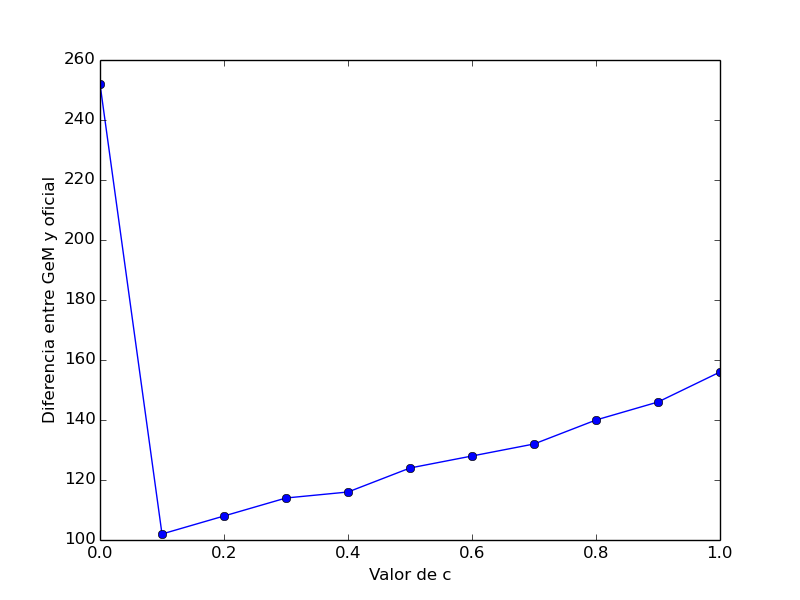
\includegraphics[width=.5\textwidth]{exp6_arg.png}}
            }
            \caption{GeM vs Primera Divisi\'on F\'utbol Argentino para $\alpha=1$}
            \label{fig:exp6_arg_1}
        \end{figure}

        \par La posición de San Martín de San Juan (13º según el puntaje
        oficial) en el ranking GeM se debe, en parte, a que le ganó a San
        Lorenzo en la fecha 3, mientras que Aldosivi (24º según el puntaje
        oficial) logró lo mismo en la fecha 10 y le gano a San Martín de San
        Juan en la fecha 22. Removiendo esos partidos sus posiciones en GeM
        bajan significativamente.

        \par De todos modos podemos observar que, para el valor de $\alpha=0.1$,
        el ranking devuelto por GeM se parece un poco más al oficial, d\'andonos
        los 6 primeros puestos que se pueden observar en el cuadro
        \ref{subfig:exp6_arg_prim}.

        \begin{figure}[H]
            \centering
            \subfloat[][Primeros Puestos\label{subfig:exp6_arg_prim}]{
                \footnotesize
                \setlength{\tabcolsep}{3pt}
                \begin{tabular}{|l|r||l|r|}
                    \hline
                    \multicolumn{2}{|c||}{GeM}&\multicolumn{2}{c|}{Oficial: 3-1-0}\\
                    \hline
                    Equipo & Puntaje & Equipo & Puntaje\\
                    \hline\hline
                    River Plate &0.0383429& San Lorenzo &50 \\
                    Boca Juniors& 0.038337& Boca Juniors &49 \\
                    San Lorenzo &0.0372973& Racing Club &46 \\
                    Racing Club &0.0363868& Rosario Central &45 \\
                    San Martín (SJ) &0.0352285& River Plate &44 \\
                    Rosario Central &0.0347587& Independiente &38\\
                    \hline
                \end{tabular}
            }\hspace{2pt}
            \subfloat[][\'Ultimos Puestos\label{subfig:exp6_arg_ult}]{
                \footnotesize
                \setlength{\tabcolsep}{3pt}
                \begin{tabular}{|l|r||l|r|}
                    \hline
                    \multicolumn{2}{|c||}{GeM}&\multicolumn{2}{c|}{Oficial: 3-1-0}\\
                    \hline
                    Equipo & Puntaje & Equipo & Puntaje\\
                    \hline\hline
                    Olimpo &0.0316438&Godoy Cruz &22\\
                    Huracán &0.0315532&Huracán &21\\
                    Godoy Cruz &0.0315278&Atlético de Rafaela &20\\
                    Atlético de Rafaela &0.0309498&Arsenal &17\\
                    Colón &0.0308694&Nueva Chicago &14\\
                    Nueva Chicago &0.0307189&Crucero del Norte &14\\
                    \hline
                \end{tabular}
            }
            \caption{GeM vs Primera Divisi\'on F\'utbol Argentino para $\alpha=0.1$}
            \label{fig:exp6_arg_2}
        \end{figure}
        \medskip

        \par De estos 6 primeros puestos de GeM, 5 efectivamente corresponden a
        esos primeros 6 lugares según el oficial (el que falta es Independiente,
        que GeM ubica 15º) y uno de ellos está en la misma posición en ambos
        rankings.

        \par Otra coincidencia notable son los últimos puestos, los cuales se
        pueden observar en el cuadro \ref{subfig:exp6_arg_ult}. Esta tabla tiene
        3 coincidencias débiles (mismos equipos en distinta posición) y una
        coincidencia exacta.\\

%%*************************************************************************
    \item En este caso, la diferencia para valores no nulos de $\alpha$ 
        es escasa, y la diferencia con el oficial en general es mucho mejor que
        para el caso del campeonato argentino. Consideramos esto relacionado al
        hecho de que hay pocos partidos en total, y a que la organización del
        torneo también se basa fuertemente en la transitividad de victorias (al
        menos en la fase final): en un Mundial, si A le ganó a B y B a C, se asume que A es
        mejor que C.

        \par Para todos los valores no nulos de $\alpha$ GeM ubicó
        correctamente como ganador a Alemania. Para $\alpha=0.1$ considero que
        el subcampeón fue Países Bajos, lo cual sorprende dado que Argentina le
        ganó ''4 a 2'' (el resultado de los penales). Evidentemente un valor tan
        bajo de $\alpha$ le da baja importancia a esto y pondera más las
        diferencias de goles de Países Bajos contra sus rivales (4 vs España, 2
        vs Chile), mucho mejores que las de Argentina (que ganó todos sus
        otros partidos por un gol de diferencia). Para todos los demás valores de
        $\alpha$, GeM identificó correctamente a Argentina como subcampeón.

        \par Las menores diferencias generales se obtuvieron para $\alpha=0.2$,
        $\alpha=0.3$ y $\alpha=0.4$ ''empatadas'' en una distancia de 50 con el
        ranking oficial de la FIFA. En estos casos sorprende la precisión de los
        resultados. Por ejemplo, observemos los primeros 8 lugares en la
        siguiente tabla, que coinciden exactamente con el ranking provisto por
        la FIFA:

        \begin{figure}[H]
            \centering
            \subfloat[][Primeros puestos $\alpha=0.4$]{
                \footnotesize
                \setlength{\tabcolsep}{3pt}
                \begin{tabular}[b]{|l|r|}
                    \hline
                    Equipo & Puntaje\\
                    \hline\hline
                    Alemania &0.0986858\\
                    Argentina &0.0764719\\
                    Países Bajos &0.0650904\\
                    Brasil &0.0480157\\
                    Colombia& 0.0419815\\
                    Bélgica &0.0405001\\
                    Francia &0.0396461\\
                    Costa Rica &0.0344357\\
                    \hline
                \end{tabular}
            }\hspace{10pt}
            \subfloat[][Diferencia en Funci\'on de $\alpha$]{
                \raisebox{-.13\height}{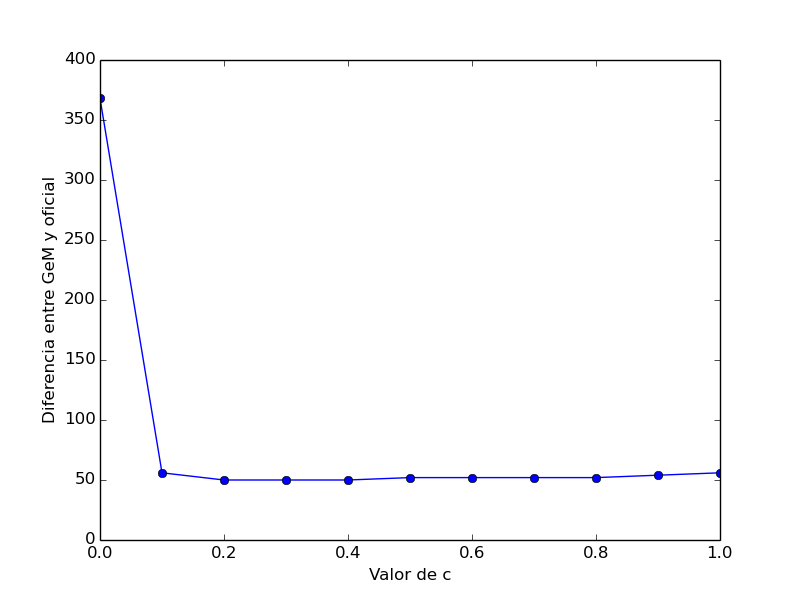
\includegraphics[width=0.5\textwidth]{exp6_2014.png}}
            }
            \caption{GeM vs Copa del Mundo 2014}
        \end{figure}

        Al consultarle su opinión al respecto de si fue o
        no penal, GeM guardó un respetuoso silencio.

%%*************************************************************************
    \item Nuevamente observamos una buena aproximación entre GeM y el ranking
        oficial. Quizás los más sorprendente es que para todos los valores no
        nulos de $\alpha$, GeM supo clasificar a Alemania Federal como el
        ganador del torneo a pesar de haber perdido por una diferencia de 5
        goles en la fase de grupos con el subcampeón Hungría. La explicación que
        le encontramos a esto se basa en que la final se disputó precisamente
        entre esos dos equipos, y Alemania Federal se consagró ganador por 3 a
        2. Esto produce que el grafo de conectividad tenga un ciclo entre esas
        dos selecciones, lo cual hace que parte del "puntaje" de Hungría vuelva
        a Alemania Federal. Todo eso sumado a la excelente campaña de este
        último en el campeonato (4 a 1 vs Turquía, 7 a 2 nuevamente vs Turquía,
        2 a 0 vs Yugoslavia y 6 a 1 vs Austria, que venía de ganar varios
        partidos también por gran diferencia) lo posiciona efectivamente como
        ganador según GeM.

        \par También para todos los valores de $\alpha$ GeM acierta en ubicar a
        Hungría como subcampeón.

        \par La menor diferencia con el ranking oficial se obtiene con
        $\alpha=0.8$ y $\alpha=0.9$. Es preciso notar que no pudimos evaluar el
        caso $\alpha=1$ por no converger para esta instancia, a diferencia de
        las dos competiciones anteriores\footnote{Sabemos por la secci\'on
        \ref{sec:introduccion} que la convergencia está asegurada solo para $0\leq\alpha <1$, pero de todos modos venimos
        ``ensayando'' con $\alpha=1$ sabiendo que dicho valor no tiene por qué hacer
        converger al m\'etodo de la potencia para nuestro $M$}.

        \par En estos dos casos, GeM acertó en los 5 primeros puestos de la
        competición, siendo estos:

        \begin{figure}[H]
            \centering
            \subfloat[][Primeros Puestos $\alpha=0.4$]{
                \footnotesize
                \setlength{\tabcolsep}{3pt}
                \begin{tabular}{|l|r|}
                    \hline
                    Equipo & Puntaje\\
                    \hline\hline
                    Alemania Federal &0.421402\\
                    Hungría &0.409884\\
                    Austria &0.0299615\\
                    Uruguay &0.0252637\\
                    Suiza &0.0169375\\
                    \hline
                \end{tabular}
            }\hspace{10pt}
            \subfloat[][Diferencia en Funci\'on de $\alpha$]{
                \raisebox{-.5\height}{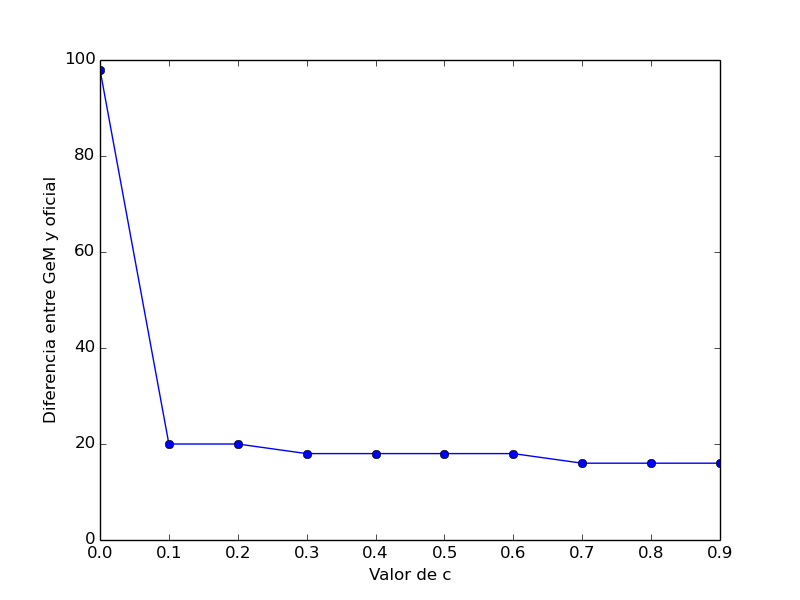
\includegraphics[width=0.5\textwidth]{exp6_1954.png}}
            }
            \caption{GeM vs Copa del Mundo 1954}
        \end{figure}
\end{enumerate}
\medskip

%%*************************************************************************
\par Lo m\'as jugoso de toda esta experimentaci\'on radica en que comparamos el
modelo GeM de rankings contra todos rankings oficiales que est\'an vigentes. El
primer resultado interesante es observar que GeM est\'a mucho m\'as cerca para
del ranking utilizado en las copas del mundo que del torneo actual del f\'utbol
argentino, y esto se ve para cualquier $\alpha\neq 0$ (el caso con $\alpha = 0$,
como ya se comentado en experimentos previos, concibe un modelo donde todos los
equipos le pueden ganar a todos con la misma probabilidad, sin importar los
resultados previos, haciendo a este par\'ametro poco interesante para analizar
por su obvia ignorancia de la realidad\footnote{¿O acaso las chances de que
Racing le gane a Crucero del Norte son las mismas de que pierda?}). A\'un as\'i,
a pesar de esta distancia, vemos que en el caso del torneo de f\'utbol
argentino, su ranking en los extremos de la ''tabla'' (particularmente en el
extremo inferior) suele ubicar a los mismos equipos que el ranking oficial. Esto
nos indica que a pesar de tener rankings muy distintos, en t\'erminos generales
ambos rankings diferencian de forma similar a los equipos ''buenos'' y
''malos''.

\par Concluyendo, vemos que GeM puede o no parecerse a otros rankings oficiales,
pero la determinaci\'on de si es mejor o peor depender\'a de qué opinen quienes
lo utilicen. Lo que si podemos afirmar es que GeM tiende a aproximarse m\'as
a los rankings oficiales (al menos los vistos) en los extremos del mismo. Es
decir, a pesar de estar a una distancia no despreciable del ranking oficial, los
equipos se\~nalados como los m\'as fuertes o mejores por ambos rankings (o los
peores) tienen varias coincidencias. Decimos entonces que, desde el punto de
vista de clasificar a un equipo como ''de los buenos'' o ''de los malos'' de la
competencia, cualquiera de los rankings dar\'ia resultados similares, pero estos
se diferencian al entrar en el detalle de qué equipo es mejor que otro.


\newpage
\subsubsection{Estabilidad de GeM}
\label{subsec:exp7}
\begin{LaTeXdescription}
    \item[Objetivo] Observar el ranking de PageRank/GeM puede sufrir variaciones
        importantes de una fecha a la otra, al recibir un set nuevo de
        informaci\'on.\\

    \item[Hip\'otesis] GeM es m\'as inestable que la puntuaci\'on oficial del
        f\'utbol.\\

    \item[Proposici\'on] Nos interesa considerar casos extremos para evaluar la
        estabilidad del ranking que devuelve GeM. El sistema de puntaje actual
        del f\'utbol tiene la caracter\'istica de ser bastante ''estable'': en
        una \'unica fecha un equipo puede ganar a lo sumo 3 puntos, lo cual
        (salvo en los comienzos de un torneo o casos de empate m\'ultiple
        dif\'iciles de encontrar en la realidad) no lo hace avanzar m\'as de 4 o
        5 posiciones.

        \par Nos interesa analizar si esta propiedad se conserva en GeM. Para
        eso, imaginemos un torneo de f\'utbol desbalanceado, es decir, un torneo
        en que al finalizar, el primer equipo tiene mucha diferencia con el
        \'ultimo\footnote{Consideramos esto desbalanceado. Si no es este el
        caso del lector, simplemente considerar una instancia que cumpla con esa
        condici\'on.}. Si en una \'ultima fecha ''inventada'', agregada
        artificialmente, el \'ultimo le ganase al primero, el m\'etodo de
        puntuaci\'on est\'andar dif\'icilmente altere demasiado el ranking.
        Queremos observar si esto ocurre con GeM.\\

    \item[M\'etodo de Experimentaci\'on] Tomamos el Campeonato de Primera B
        Nacional 2013/14, en el cual Banfield (1º) termin\'o con 78 puntos
        mientras que Villa San Carlos (22º y \'ultimo) termin\'o con 24.
        Generamos una fecha artificial extra en la que Villa San Carlos le gana
        a Banfield. El ranking oficial no cambiar\'ia, dado que con 27
        puntos Villa San Carlos seguir\'ia \'ultimo. De confirmarse nuestra
        hip\'otesis, esperar\'iamos ver un cambio en la posición que GeM le
        asigna a Villa San Carlos. En este caso, variando la cantidad de goles,
        estudiamos cu\'anto se alterar\'ia el resultado si la victoria fuese
        m\'as abultada. El valor de $\alpha$ usado fue de 0.85.\\

    \item[Resultados, an\'alisis y discusi\'on]
\end{LaTeXdescription}

\par Se confirmó la hipótesis. Efectivamente GeM altera el ranking por una
simple victoria por 1 a 0, aunque Villa San Carlos sigue último. Esto se debe a
que el puntaje GeM de Banfield cae y el de VSC sube, alterando a los demás
equipos que ganaron o perdieron contra alguno de ellos.

\begin{figure}[H]
    \centering
    \subfloat[][Distancia GeM Adulterado vs Oficial/GeM\label{subfig:exp7_dist_ranks}]{
        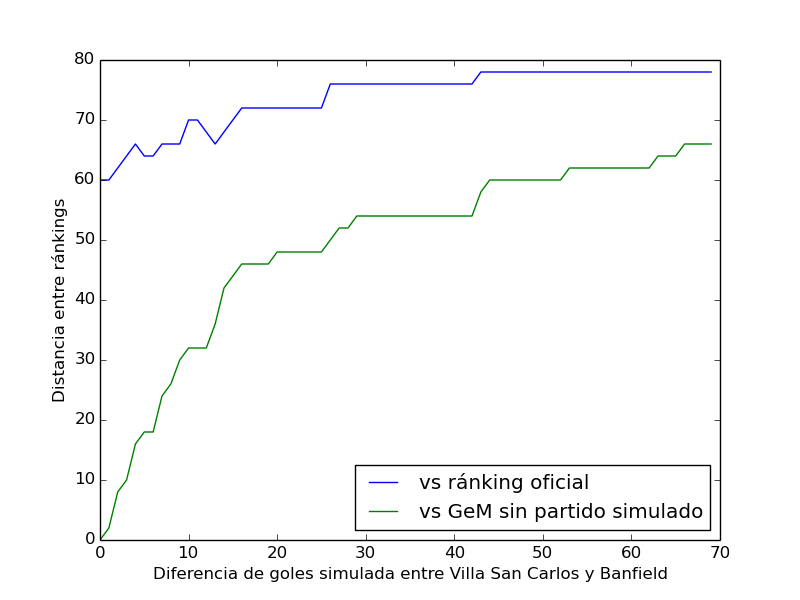
\includegraphics[width=.45\textwidth]{exp7_diferencia_ranks_funcion_goles.png}
    }\hspace{2pt}
    \subfloat[][Posición de Villa San Carlos en GeM Adulterado\label{subfig:exp7_pos_vsc}]{
        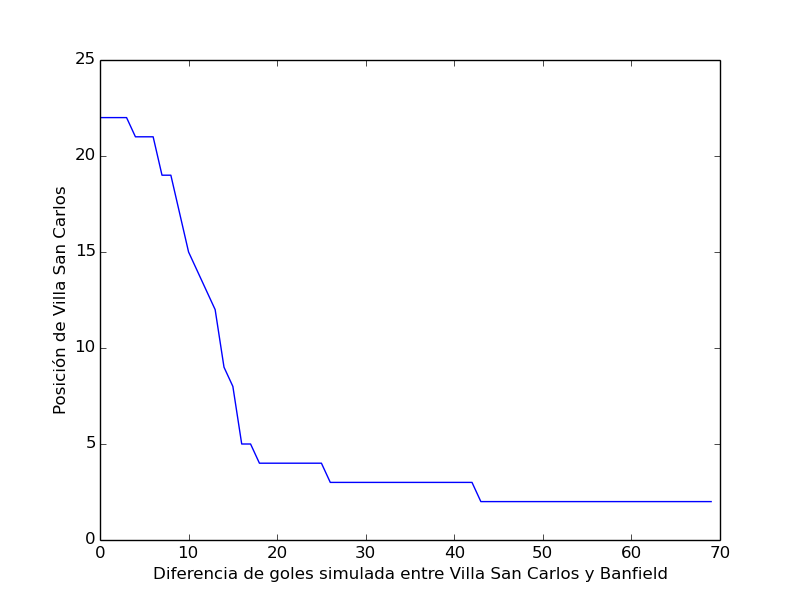
\includegraphics[width=.45\textwidth]{exp7_poscion_villa_san_carlos.png}
    }
    \caption{Consecuencias de introducir un partido artificial}
\end{figure}

\par Alcanza con una victoria de 4 a 0 para que Villa San Carlos deje el último
lugar. Y con una victoria de 43 a 0 pasa a estar en 2do lugar. Si esto parece
irreal, considerar el récord del fútbol profesional de goles en un mismo
partido: \emph{AS Adema 149 - 0 SO l'Emyrne}, el 31 de octubre de 2002 por la
\emph{THB Champions League de Madagascar}\footnote{En honor a la verdad, este
resultado fue alcanzado por goles en contra por protesta contra el arbitraje.
El resultado ``honesto'' más abultado fue \emph{Arbroath FC 36 - 0 Bon Accord
FC}, el 12 de septiembre de 1885 por la Copa Escocesa 1885-86 y, más
recientemente, el conocido \emph{Australia 31 - 0 Samoa Americana}, el 11 de
abril de 2001, por la clasificación al Mundial de Fúbol Corea-Japón 2002}.

\par En la figura \ref{subfig:exp7_pos_vsc} se puede observar la posición de
Villa San Carlos en función de la cantidad de goles del partido artificial. En
la figura \ref{subfig:exp7_dist_ranks} se puede observar la diferencia entre
rankings producida por el partido simulado en función de la cantidad de goles
del partido. Se observa claramente la ``inestabilidad'' de la que hablábamos:
por los resultados de un simple partido GeM puede alterar el orden en un factor
grande. Consideramos que esta no es una propiedad deseable del sistema, al
menos no para el fútbol: hay muchos factores que influyen en un resultado,
independientemente de la calidad de los competidores (azar, arbitraje, clima,
estado del campo, etc.). Un equipo ``malo'' no debería dejar de serlo solo por
haber haber tenido suerte (o incluso por haber hecho un único buen partido)
contra un equipo ``bueno'', o porque su rival haya hecho un partido malo.

\par El próximo experimento apunta a dejar aún más en evidencia esta situación.


\newpage
\subsection{Caso Particular GeM}
\label{subsec:exp8}
\begin{LaTeXdescription}
    \item[Objetivo] Analizar cuan ``justo'' es GeM, para un caso particular en
        el cual no haya dudas sobre lo que es justo y lo que no\footnote{O que
        haya muy poca probabilidad de que haya dudas al respecto.}.\\

    \item[Proposici\'on] Nos interesa analizar cu\'an ''justo'' es GeM para
        cierta definici\'on de justicia. Consideremos el caso de un torneo en
        que el equipo A le gana a todos los equipos salvo a B, y B pierde todos
        los partidos salvo el que le gana a A. Bajo nuestra definición de
        ''justicia'' o ''equidad'', o un aspecto de ella, A deber\'ia estar
        seguro por encima de B y B no deber\'ia estar por encima de muchos
        equipos (ya que perdi\'o contra todos). Observamos que en el caso del
        f\'utbol y su ránking 3-1-0 (o el esquema antiguo, 2-1-0) efectivamente
        B estar\'ia en la \'ultima posici\'on y A estar\'ia en la primera
        (eventualmente compartiendo dichas posiciones con alg\'un otro equipo).
        Entendemos entonces que este caso particular el ranking 3-1-0 es
        ''justo'' en este aspecto. Pero intu\'imos que esto no ser\'a lo que
        ocurra con GeM, ya que en el grafo de la instancia, A tiene un \'unico
        eje saliente (hacia B) y 18 entrantes, con lo cual su arista deber\'ia
        hacer subir mucho a B en el ranking.\\

    \item[Hip\'otesis] PageRank/GeM no es ''justo'' en cuanto al aspecto
        mencionado.\\

    \item[M\'etodo de Experimentaci\'on] Generamos una instancia de 20 equipos
        todos contra todos, donde existen A y B como se describieron. Entre los
        dem\'as equipos hacemos que el ganador sea aleatorios (con semilla =
        5). Todos los partidos terminan 1 a 0. Ejecutamos GeM y observamos el
        ranking final para diferentes valores de $\alpha$ (el factor de
        navegaci\'on).

    \item[Resultados, an\'alisis y discusi\'on] Lo primero que observamos es que B no ascendió al primer lugar para ningún valor de $\alpha$, lo cual era esperable dados los resultados del experimento 7 pero no deja de darnos cierta ``tranquilidad''. Sin embargo, y como se puede ver en la figura \ref{fig:exp8_posB}, la posición del equipo B sí mejora significativamente ya para valores pequeños de $\alpha$: ya un valor de $\alpha = 0.1$ deja a B 6to en el ránking, y a partir de $\alpha = 0.4$ pasa a estar 2do. Consideramos entonces que se confirmó nuestra hipótesis en el sentido de que GeM no es ``justo'' en un caso del estilo. Como ya postulamos en el experimento 7, no parece ``justo'' que un equipo prácticamente invicto que tuvo un ``mal día'' le permita a otro equipo salir 2do en una competencia en la que perdió con cuanto rival se cruzó.
    
    Podemos concluir entonces que los valores más ``justos'' de $\alpha$ serían los más bajos, dado que le dan menos importancia a estas situaciones extrañas pero perfectamente posibles en cualquier deporte.
    
\end{LaTeXdescription}

\begin{wrapfigure}{l}{0.5\textwidth}
    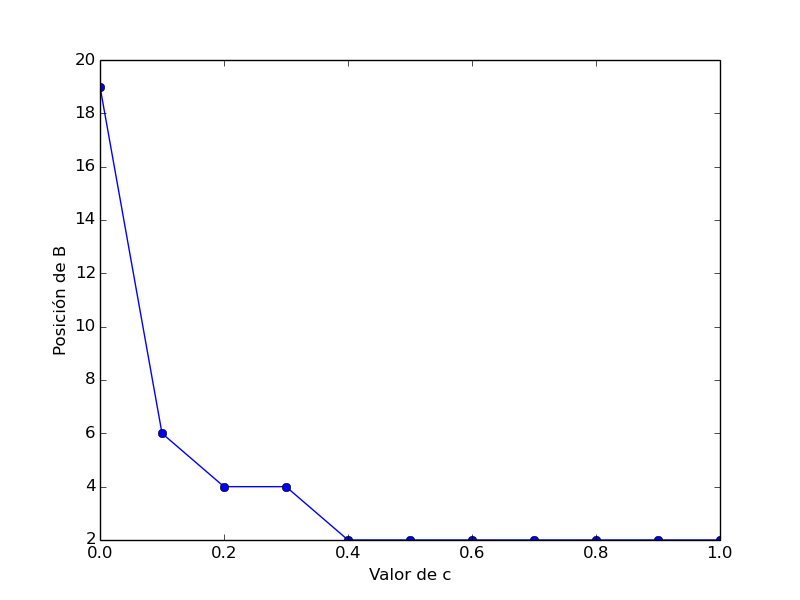
\includegraphics[width=0.5\textwidth]{exp8_posicion_B.png}
    \caption{Posici\'on del equipo B en el ranking en funci\'on del factor
        $\alpha$ ($c=\alpha$)}
    \label{fig:exp8_posB}
\end{wrapfigure}
\noindent

%---------------------------------------------------------------

    \FloatBarrier

%\newpage
%\section{Resultados}
%    % TODO
% Deben incluir los resultados de los experimentos, utilizando el formato mas adecuado
% para  su  presentacion.   Deberan  especicar  claramente  a  que  experiencia  corresponde
% cada resultado.  No se incluiran aqu corridas de maquina.
\subsection{Performance}
\subsubsection{Performance de los m\'etodos en funci\'on de la discretizaci\'on para una instancia}
Utilizamos una heur\'istica para poder determinar mejor el orden c\'ubico de la curva resultado. Sea $f(x)$ el valor del tiempo de c\'omputo, graficar $f(x)/x^k$, siendo $k \in \left[ 2, 3, 4 \right] $ . De ser $f(x)$ de orden c\'ubico, esperar\'iamos que para el polinomio de orden 2 el resultado sea una funci\'on creciente, para el de orden 3 el resultado se asemeje a una constante y para el de orden 4, una funcion decreciente.

\begin{center}
\textbf{1 instancia por archivo de test}\\
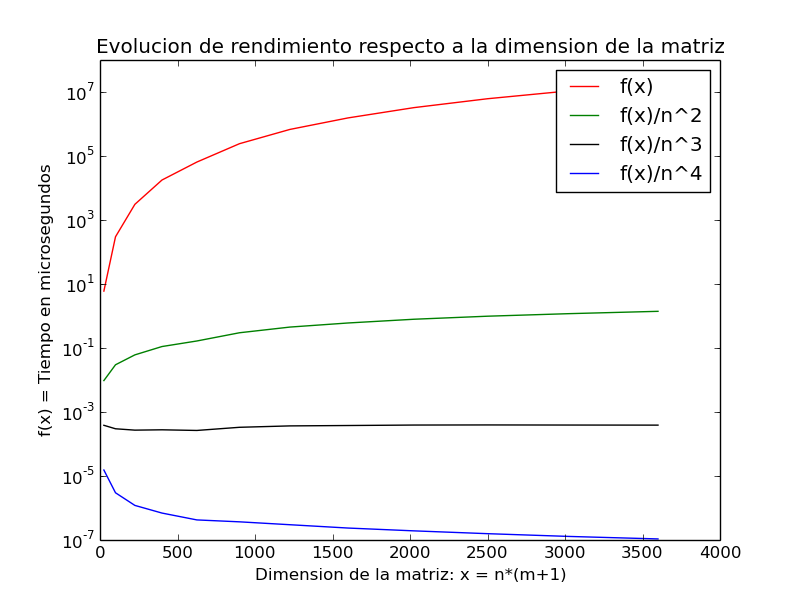
\includegraphics[scale=0.35]{experimentos2a_2b/tiempos_nm_fitteo_1_inst/eliminacion_gaussiana_time_consumed.png}
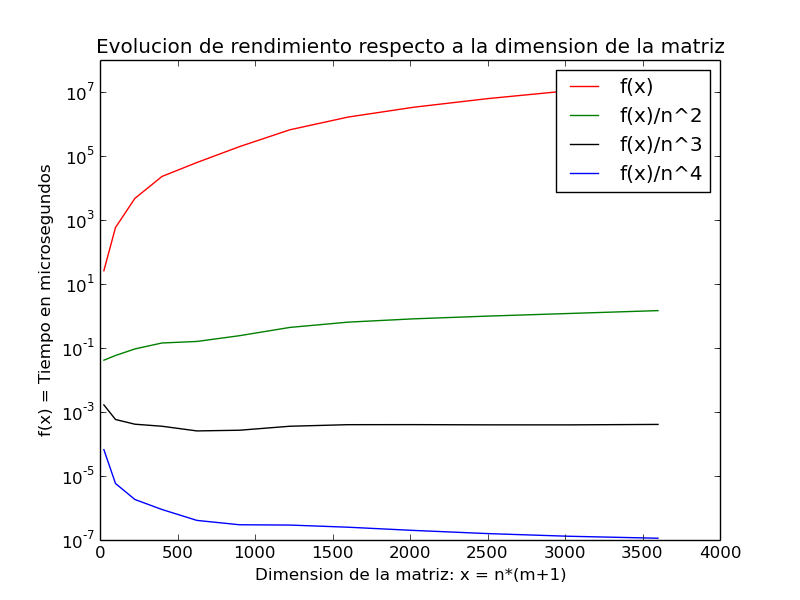
\includegraphics[scale=0.35]{experimentos2a_2b/tiempos_nm_fitteo_1_inst/factorizacion_lu_time_consumed.png}
\end{center}

A pesar de ser una heur\'istica, podemos corroborar que la curva sobre cubo se asemeja mucho a una constante, mientras que al cuadrado y a la cuarta funciones crecientes y decrecientes, respectivamente. Por lo que podemos decir que probamos emp\'iricamente que los algoritmos son del orden c\'ubico.

\subsubsection{Performance de EG vs LU variando la cantidad de instancias y la granularidad de la discretizacion}

Para comenzar esta seccion, compararemos la performance de EG vs LU variando las discretizaciones, con archivos de entrada de una sola instancia. A continuacion se presentan los graficos de comparación entre EG y LU, en diferentes escalas.

\begin{center}
\textbf{1 instancia por archivo de test}\\
\includegraphics[scale=0.35]{experimentos2a_2b/tiempos_nm_fitteo_1_inst/gauss_vs_lu_time_consumed_abs.png}
\includegraphics[scale=0.35]{experimentos2a_2b/tiempos_nm_fitteo_1_inst/gauss_vs_lu_time_consumed_log.png}
\end{center}

Dado que factorizacion LU, es identico a EG, pero guardando los coeficientes en la matriz L, tiene sentido que para una sola instancia sea mas costoso realizar la factorizacion lu y resolver el sistema que simplemente resolver usando EG.

\vspace{0.5cm}

A continuacion, se presentan graficos comparativos entre LU y EG para distintas cantidades de instancias. Lo que se observa es que, la brecha entre EG y LU se acentúa cada vez más a medida que aumenta la cantidad de instancias(ver gráficos con escala lineal). Esto se debe a que la complejidad teorica de resolver k instancias (misma matriz A, distinto vector b, en un sistema Ax=b) usando EG es $\mathcal{O}( k * (n + m)^3 )$. Por otro lado, la complejidad de resolver k instancias usando LU es $\mathcal{O}((n + m)^3 + k*(n + m)^2)$, es decir: Complejidad cúbica para hallar la descomposicion LU, y luego $k$ resoluciones de los sistemas triangulares $Ly=b$ y $Ux=y$ que cuestan orden cuadrático cada uno. 

\begin{center}
\textbf{10 instancias por archivo de test}\\
\includegraphics[scale=0.35]{experimentos2a_2b/gauss_vs_lu_10_inst/gauss_vs_lu_time_consumed_abs.png}
\includegraphics[scale=0.35]{experimentos2a_2b/gauss_vs_lu_10_inst/gauss_vs_lu_time_consumed_log.png}
\end{center}

\begin{center}
\textbf{50 instancias por archivo de test}\\
\includegraphics[scale=0.35]{experimentos2a_2b/gauss_vs_lu_50_inst/gauss_vs_lu_time_consumed_abs.png}
\includegraphics[scale=0.35]{experimentos2a_2b/gauss_vs_lu_50_inst/gauss_vs_lu_time_consumed_log.png}
\end{center}

\begin{center}
\textbf{150 instancias por archivo de test}\\
\includegraphics[scale=0.35]{experimentos2a_2b/gauss_vs_lu_150_inst/gauss_vs_lu_time_consumed_abs.png}
\includegraphics[scale=0.35]{experimentos2a_2b/gauss_vs_lu_150_inst/gauss_vs_lu_time_consumed_log.png}
\end{center}

\begin{center}
\textbf{500 instancias por archivo de test}\\
\includegraphics[scale=0.35]{experimentos2a_2b/gauss_vs_lu_500_inst/gauss_vs_lu_time_consumed_abs.png}
\includegraphics[scale=0.35]{experimentos2a_2b/gauss_vs_lu_500_inst/gauss_vs_lu_time_consumed_log.png}
\end{center}

Tambien se observa en los graficos con escala logaritmica que la brecha entre EG y LU para una cantidad de instancias fija se acentua a medida que se aumenta el tamaño de la matriz del sistema, pues el ratio LU/EG decrece. Creemos que esto se debe a que al dejar k fijo y aumentar $n+m$, tenemos que $\mathcal{O}((n + m)^3 + k*(n + m)^2)$ es mas pequeño que $\mathcal{O}(k*(n + m)^3)$ en terminos empíricos. 

\textbf{Consideraci\'on Adicional:} 

Luego de la experimentacion, se nos ocurrio una optimizacion de la implementaci\'on de los algoritmos, se agreg\'o la siguiente sentencia condicional al código de EG y la parte de triangulacion de LU:

\begin{lstlisting}
			.
			.
			.
for (int j = i+1; j < numfilas; j++) {

            if (abs(_A[j][i]) < EPSILON) {
                continue;
            }
			.
			.
			.
\end{lstlisting}

Es decir, si el elemento a analizar de la matriz es un cero(con tolerancia epsilon, en nuestro caso $exp(10, -9)$), el algoritmo no realiza el c\'alculo del coeficiente multiplicador ni tampoco opera sobre la fila multiplicando cada elemento por \'este. Al agregar esta sentencia y realizar los experimentos de fitteo de orden de complejidad, obtuvimos como resultado que la complejidad emp\'irica de ambos algoritmos era de orden cuadr\'atico. Creemos que esto se debe a la condición banda de la matriz, y que en muchos casos esta condición de corte evita que el algoritmo ingrese en la tercera iteracion anidada.

\subsection{Diferencia numérica de soluciones entre EG y LU}
En esta sección se mostraran los resultados de comparar las soluciones a un mismo sistema de ecuaciones $Ax=b$ usando LU y EG. Se realizo una variación en el tamaño de la matriz del sistema para ver la evolucion de las mediciones.\\

\vspace{0.3cm}

Los parámetros utilizados para el experimento fueron:
\begin{itemize}
	\item \textbf{Temperaturas internas y externas:}  externas(1500) e internas(100) \textbf{constantes} en todos los tests. 
	\item \textbf{Radio interno:} 200
	\item \textbf{Radio externo:} 400
	\item \textbf{Tamaño n de la matriz $A \in \mathbb{R}^{n \times n}$:} $[10^2\dots130^2]$
	\item \textbf{Isoterma buscada:} 500
\end{itemize}

No se mostrará ningun gráfico porque todas las mediciones de diferencia dieron cero, es decir:

\begin{itemize}
    \item $\norm{ x - \hat{x} }_\infty = 0.0 $
    \item $\norm{ x - \hat{x} }_2 = 0.0 $ 
\end{itemize}

Dado este sorprendente resultado a primera vista, hicimos un análisis mas fino del codigo y llegamos a algunas conclusiones:
\begin{itemize}
	\item El código de la resolución del problema es identico en ambos métodos desde la lectura de la entrada hasta el armado del sistema $Ax=b$, con lo cual no puede haber diferencia numérica en este tramo.
	\item El código de factorizacion lu y eliminacion gaussiana es \texttt{idéntico} salvo que LU guarda los multiplicadores en otra matriz L, tambien de precision doble, con lo cual lo único que podria acarrear LU contra EG en este tramo es el almacenamiento con error de los coeficientes.
	\item LU tambien podría acarrear error al realizar las 2 resoluciones de sistemas triangulares(contra una sola de EG)
\end{itemize}

Sin embargo, en los casos planteados esto no ocurre. Como futuro trabajo, se podrian fabricar casos de test muy especificos donde se fuercen errores numericos clásicos. (ie. sumas con números de distinto orden, restas con numeros muy cercanos, etc.) en las operaciones de resolucion de los sistemas triangulares, se esperaría que LU acarree mas error ya que realiza mas operaciones para resolver el sistema original $Ax=b$.

\subsection{Evolución estimación de la isoterma y temperatura}
Se presentarán los resultados de los experimentos en el mismo orden en que fueron planteados en la sección de desarrollo. Se realizará el análisis de los mismos en este mismo apartado.
\begin{enumerate}
	\item \begin{itemize}
				\item \textbf{Temperaturas internas y externas:} aleatorias uniformes entre $[50\dots200]$ y $[1450\dots1550]$, pero fijas entre tests.
				\item \textbf{Radio interno:} 200
				\item \textbf{Radio externo:} 400
				\item \textbf{Cantidad radios:} $[5\dots100]$
				\item \textbf{Cantidad ángulos:} 100
				\item \textbf{Isoterma buscada:} 500
			\end{itemize}
Se adjunta con el trabajo práctico un video que expone la evolución del sistema mientras se incrementa la cantidad de radios. Expondremos estáticamente algunos frames, pero es conveniente ver el video primero. Se encuentra en la misma carpeta que el pdf. (variación\_radial\_isomap.mp4, variación\_radial\_heatmap.mp4).

\vspace{0.5cm}

  	\textbf{Variación de la estimación de la isoterma entre 5 y 6 radios de discretización}\\
	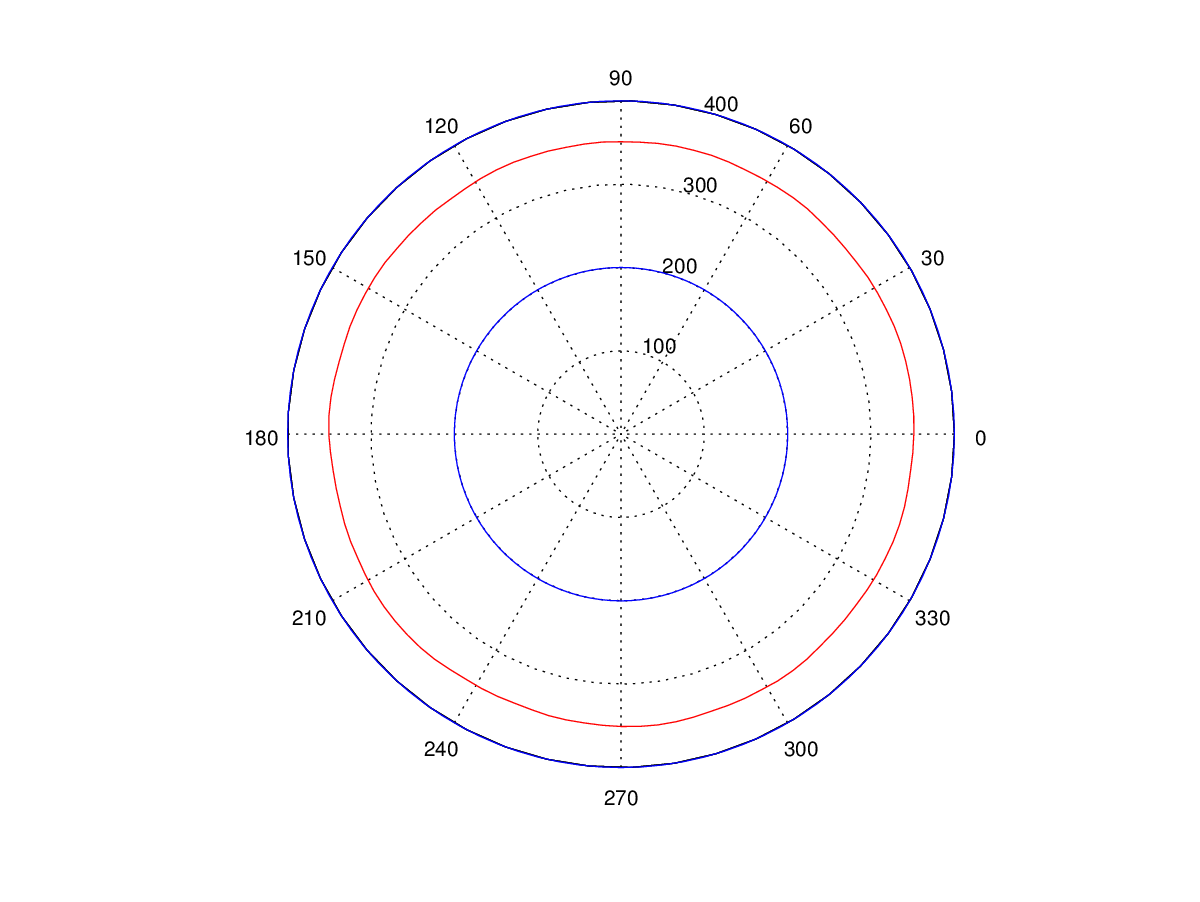
\includegraphics[scale=0.35]{experimentos1a_1b/evolucion_posicion_isoterma_temperatura/test2/test6_006_radios_inst_001_isomap.png}
	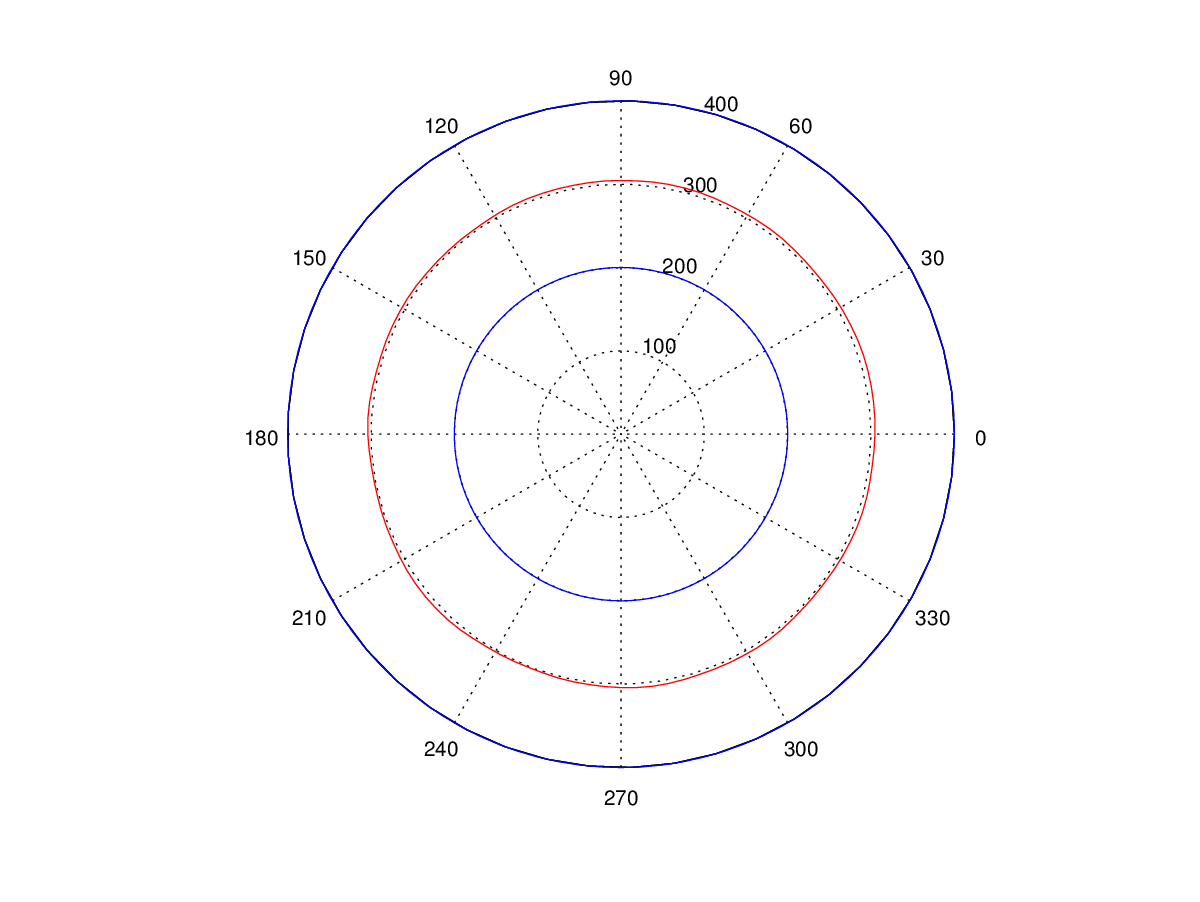
\includegraphics[scale=0.35]{experimentos1a_1b/evolucion_posicion_isoterma_temperatura/test2/test6_007_radios_inst_001_isomap.png}
	
  	\textbf{Variación de la temperatura entre 6 y 7 radios de discretización}\\
	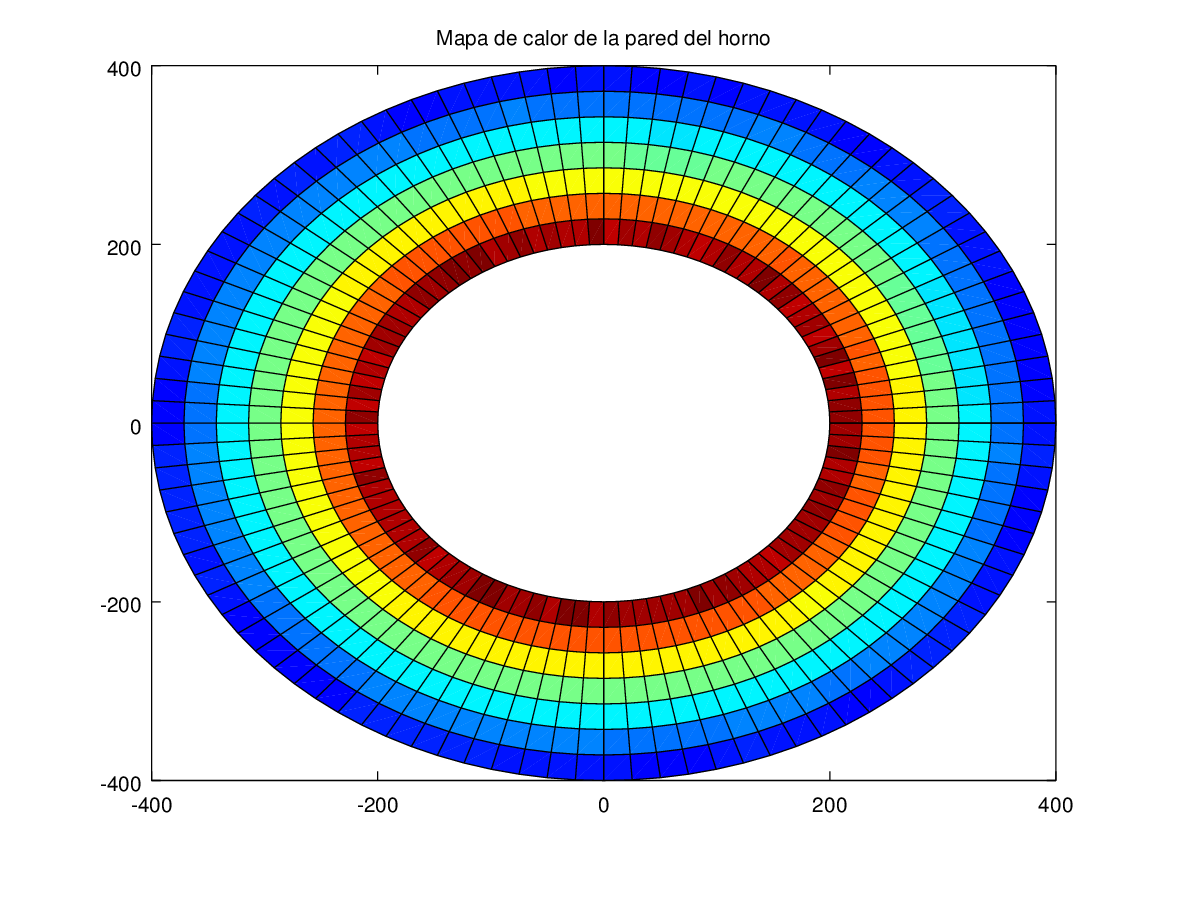
\includegraphics[scale=0.35]{experimentos1a_1b/evolucion_posicion_isoterma_temperatura/test2/test6_006_radios_inst_001_heatmap.png}
	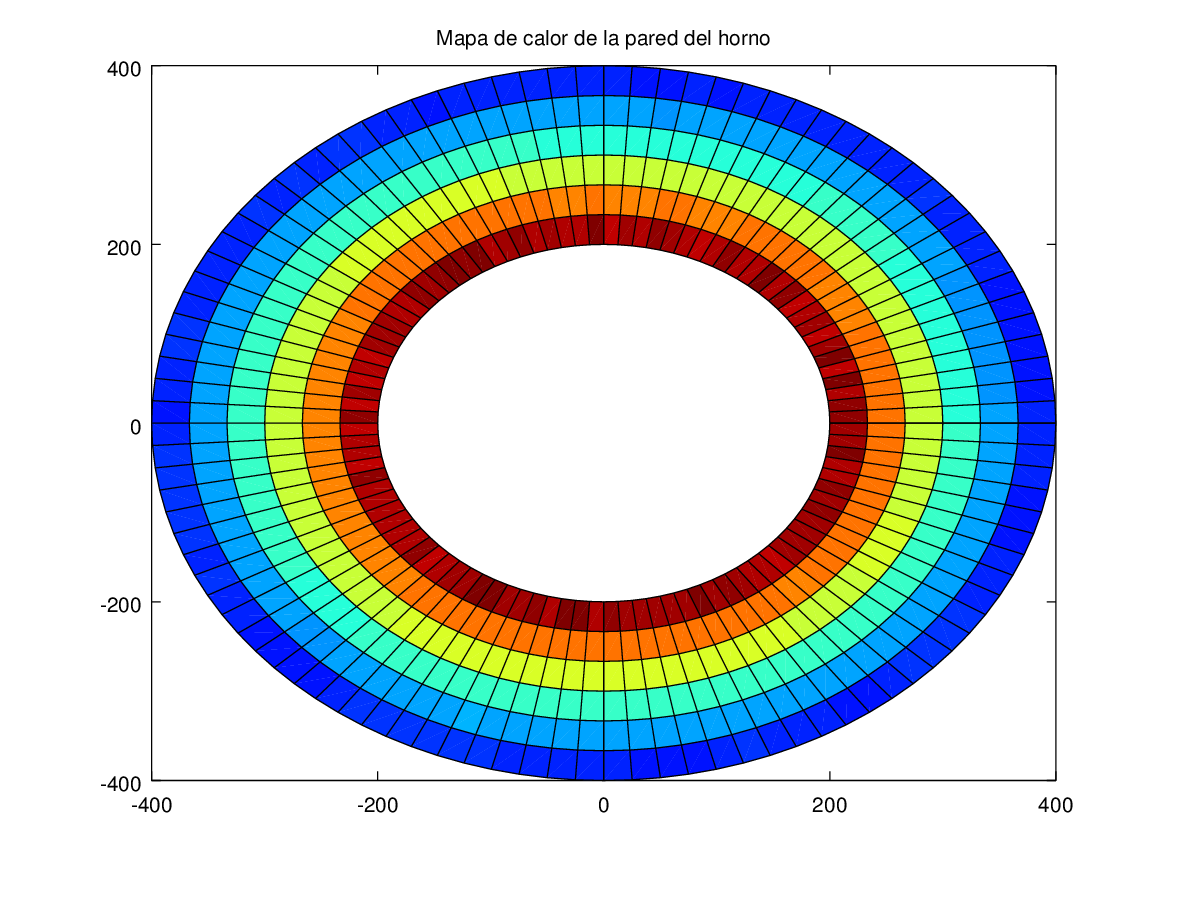
\includegraphics[scale=0.35]{experimentos1a_1b/evolucion_posicion_isoterma_temperatura/test2/test6_007_radios_inst_001_heatmap.png}

 	\textbf{Variación de la estimación de la isoterma entre 99 y 100 radios de discretización}\\
	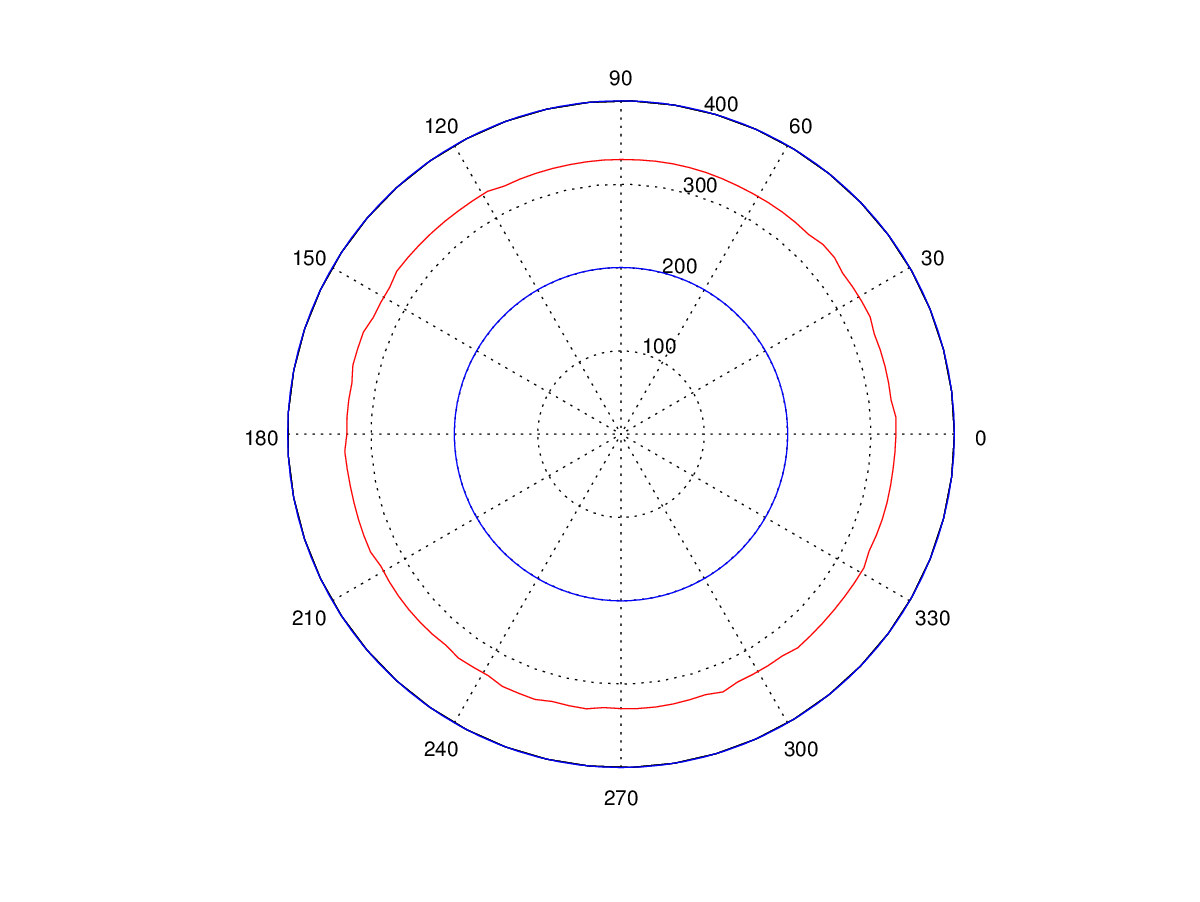
\includegraphics[scale=0.35]{experimentos1a_1b/evolucion_posicion_isoterma_temperatura/test2/test6_099_radios_inst_001_isomap.png}
	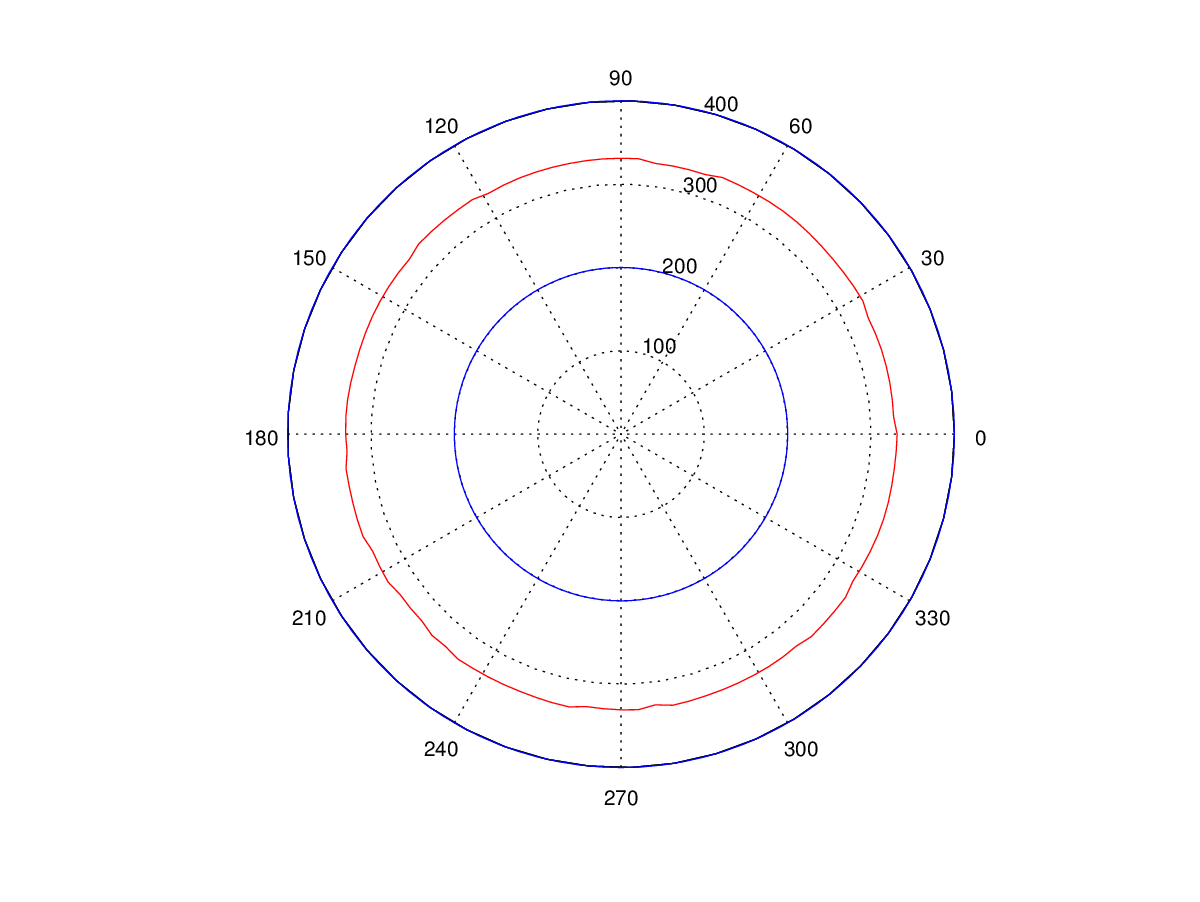
\includegraphics[scale=0.35]{experimentos1a_1b/evolucion_posicion_isoterma_temperatura/test2/test6_100_radios_inst_001_isomap.png}
	
	\textbf{Variación de la temperatura entre 99 y 100 radios de discretización}\\
	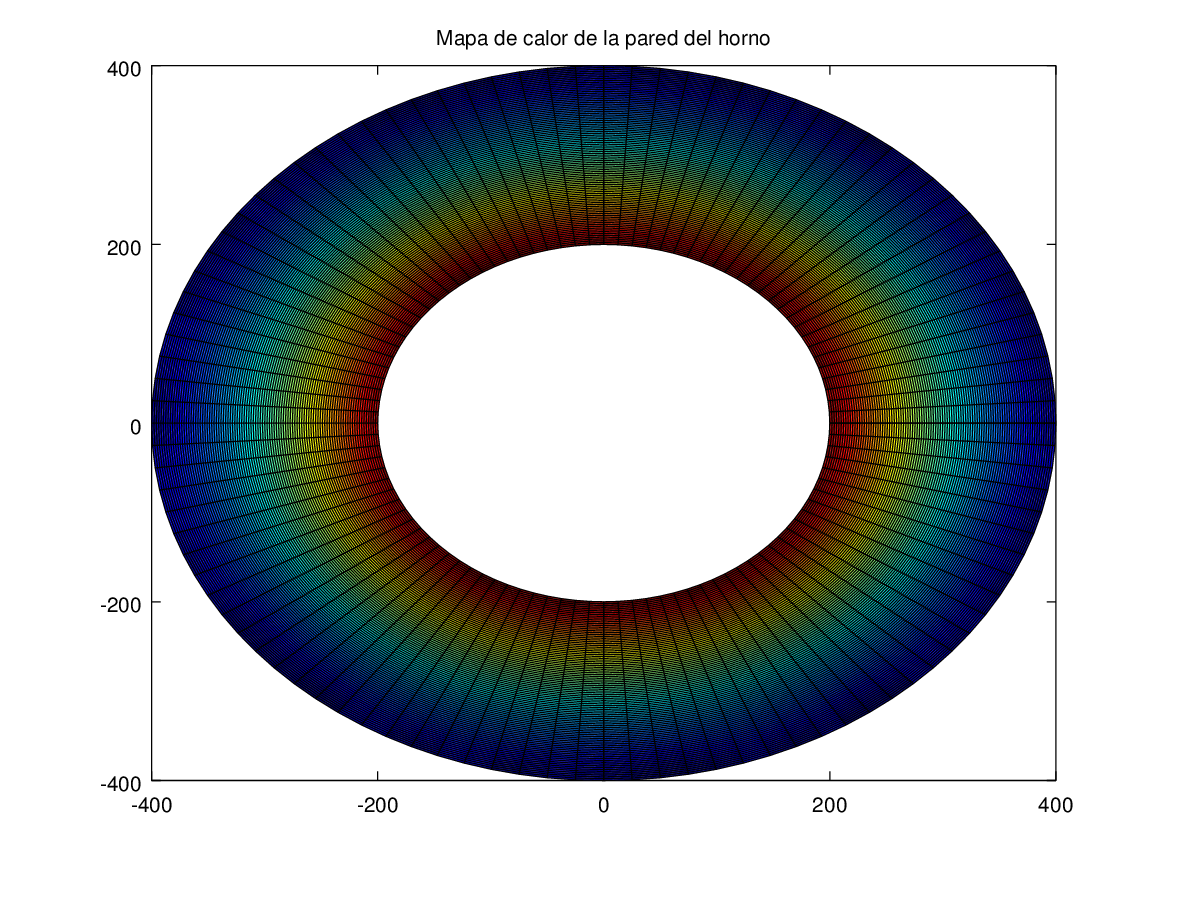
\includegraphics[scale=0.35]{experimentos1a_1b/evolucion_posicion_isoterma_temperatura/test2/test6_099_radios_inst_001_heatmap.png}
	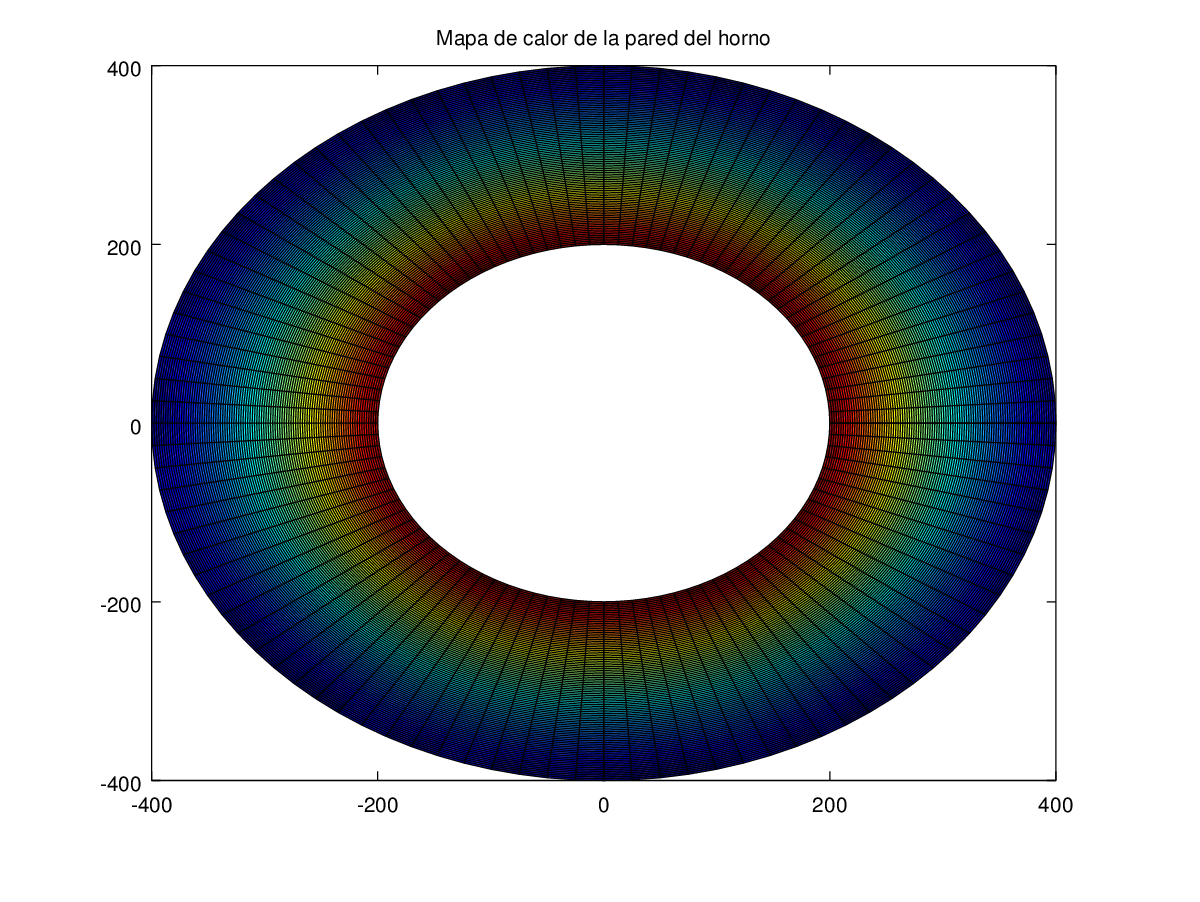
\includegraphics[scale=0.35]{experimentos1a_1b/evolucion_posicion_isoterma_temperatura/test2/test6_100_radios_inst_001_heatmap.png}

\vspace{0.5cm}

Se observa es que a medida que se aumenta la cantidad de radios de la discretización, la variación radial de la curva de la isoterma disminuye entre tests, es decir, se hace más fina la estimación, de forma tal que entre $i$ e $i+1$ radios la diferencia de la posición de la isoterma es menor a medida que $i$ crece. Para ver mejor esto se graficaron, para cada test de $i$ cantidad de radios de la discretización, el máximo y el promedio radial de la isoterma.

	\textbf{Evolución de la variación radial de la isoterma con cantidad creciente de radios}\\
	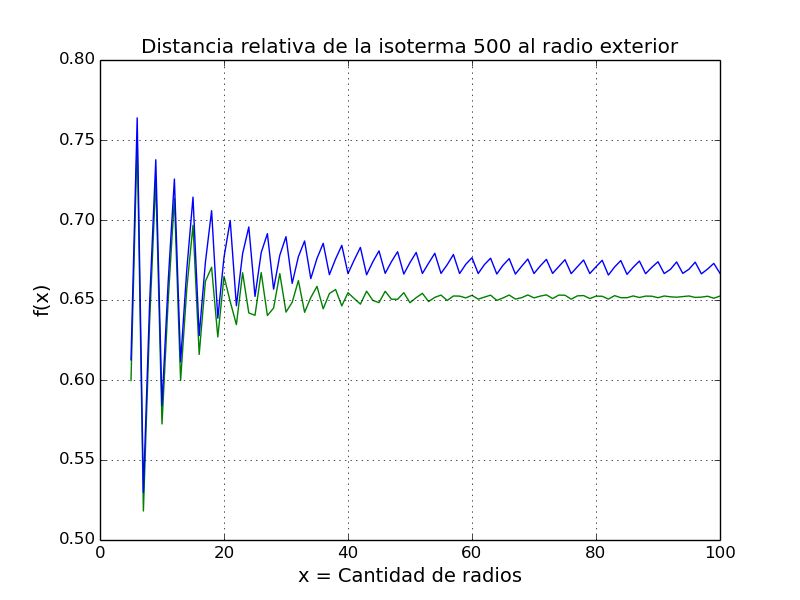
\includegraphics[scale=0.5]{experimentos1a_1b/evolucion_estimacion_seguridad_isoterma/100ang_5to100radios.png}\\


Para evitar distorsiones en el experimento anterior, se realizo otro muy similar al anterior pero con condiciones de borde \textbf{constantes e iguales}.
\begin{itemize}
	\item \textbf{Temperaturas internas y externas:} constantes, 100 y 1500. Esto es para que tenga la misma solución cada test del experimento.
	\item \textbf{Radio interno:} 200
	\item \textbf{Radio externo:} 400
	\item \textbf{Cantidad radios:} $[10\dots200]$
	\item \textbf{Cantidad ángulos:} 75
	\item \textbf{Isoterma buscada:} 500
\end{itemize}

No expondremos los resultados acerca de la evolucion de la temperatura y posicion de la isoterma, pues son similares al experimento anterior, la isoterma converge a medida que aumenta la cantidad de radios utilizada en la discretización. Al ser temperaturas constantes en este caso, la isoterma es un círculo perfecto. En el experimento anterior, la isoterma tenia pequeñas(casi imperceptibles) irregularidades dadas las condiciones aleatorias(con baja varianza) de borde.

\vspace{0.3cm}

Respecto al gráfico del promedio/maximo de la isoterma a medida que aumentan los radios, se tiene lo siguiente.

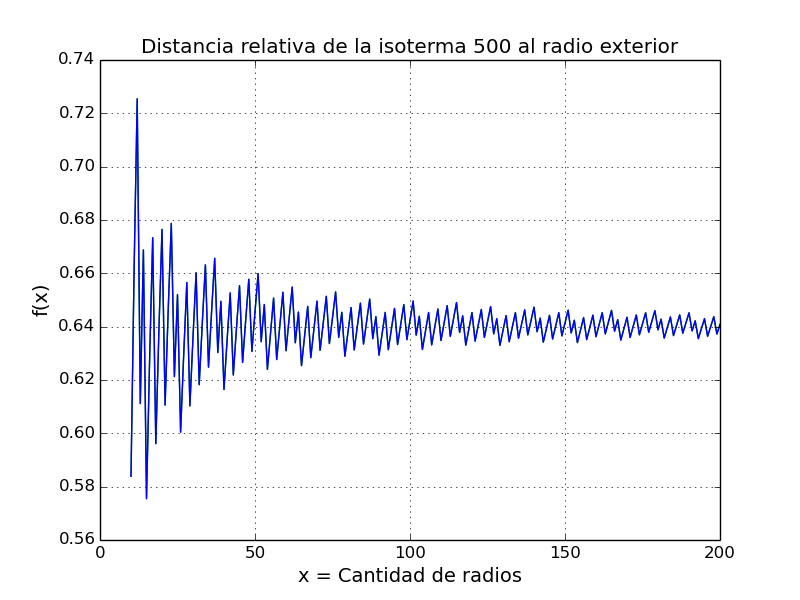
\includegraphics[scale=0.5]{experimentos1a_1b/evolucion_estimacion_seguridad_isoterma/75ang_10to200rad_evol_maxpromradio.png}\\
\textbf{Nota:} Al ser las condiciones de borde iguales, la isoterma tiene radio constante para cada experimento, con lo cual maximo y promedio coinciden, con lo cual se ve una sola curva.

\vspace{0.2cm}

Se puede ver que, al igual que en el experimento anterior, al aumentar la cantidad de radios, la posicion de la isoterma converge. Tambien se observa que en ambos experimentos, la posicion relativa de la isoterma converge aproximadamente a 0.64/0.66, lo cual tiene sentido ya que el experimento anterior tenia temperaturas aleatorias uniformes, pero \texttt{casi} alrededor de las temperaturas fijadas en el segundo experimento.\\

	\item \begin{itemize}
					\item \textbf{Temperaturas internas y externas:} constantes, 100 y 1500. Esto es para que tenga la misma solución cada test del experimento.
					\item \textbf{Radio interno:} 200
					\item \textbf{Radio externo:} 400
					\item \textbf{Cantidad radios:} 50
					\item \textbf{Cantidad ángulos:} $[5\dots50]$
					\item \textbf{Isoterma buscada:} 500
				\end{itemize}
	Se adjunta con el trabajo práctico un video que expone la evolución del sistema mientras se incrementa la cantidad de radios. Expondremos estáticamente algunos frames, pero es conveniente ver el video primero. Se encuentra en la misma carpeta que el pdf. (variación\_angular\_isomap.mp4, variación\_angular\_heatmap.mp4).

	\vspace{0.5cm}
	  	\textbf{Variación de la estimación de la isoterma entre 5 y 6 ángulos de discretización}\\
		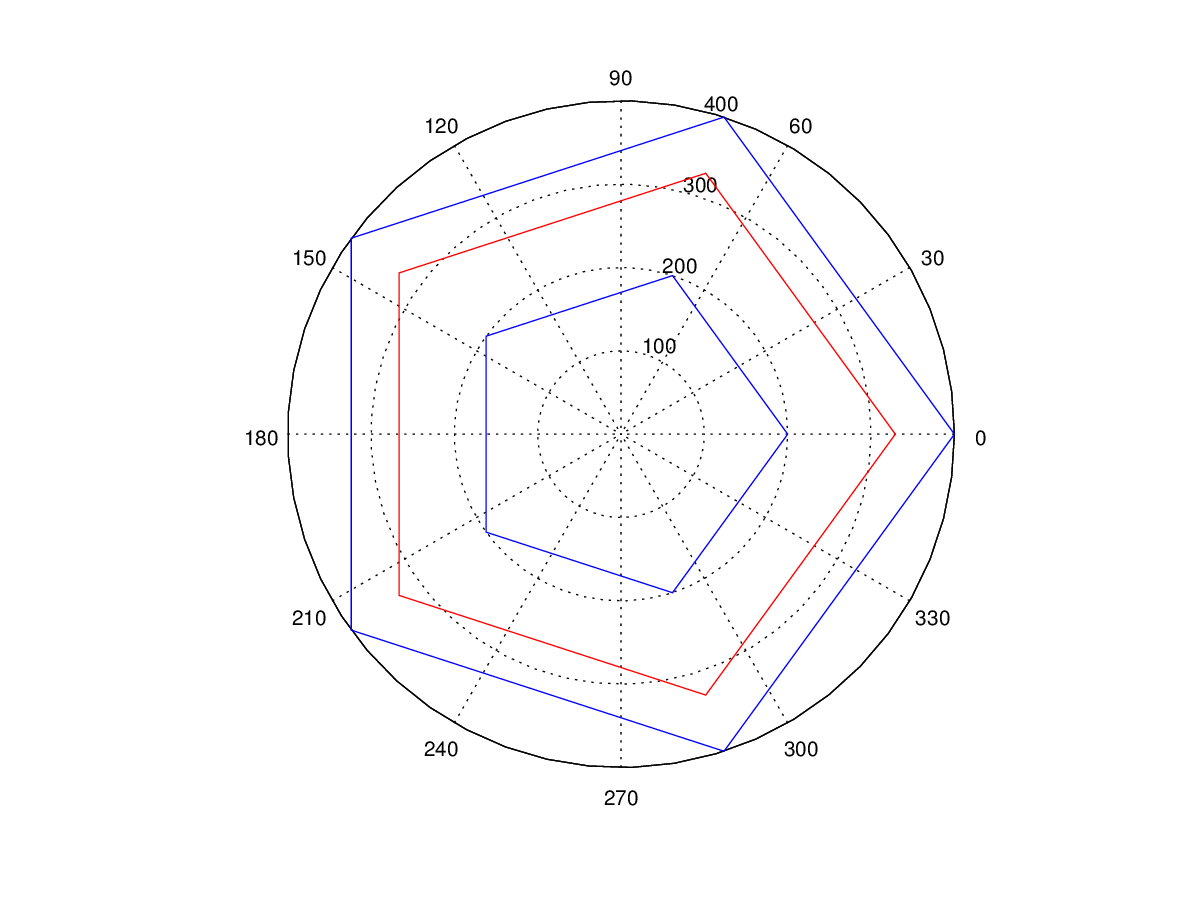
\includegraphics[scale=0.35]{experimentos1a_1b/evolucion_posicion_isoterma_temperatura/variacion_angulos_radio_fijo_se_suaviza_isoterma/test10_050_radios_005_angulos_inst_001_isomap.png}
		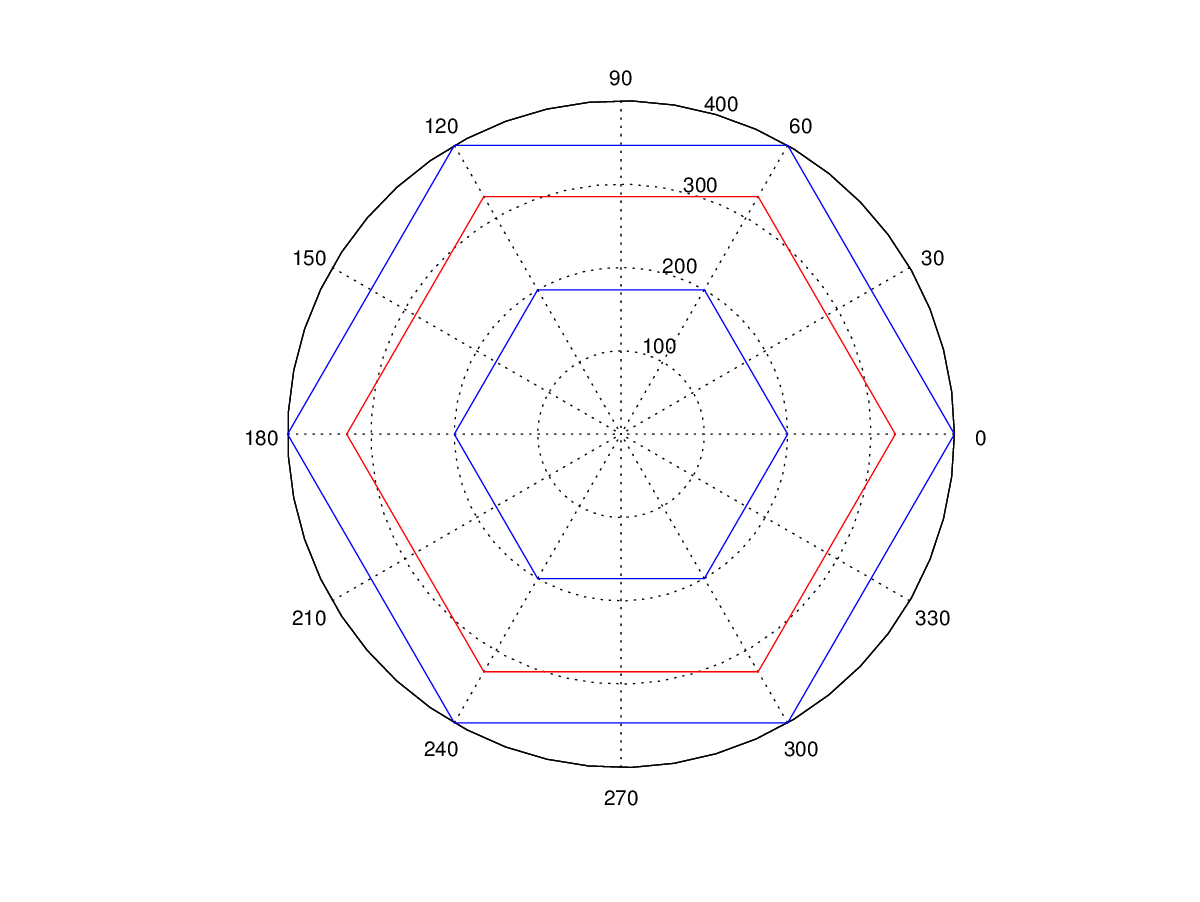
\includegraphics[scale=0.35]{experimentos1a_1b/evolucion_posicion_isoterma_temperatura/variacion_angulos_radio_fijo_se_suaviza_isoterma/test10_050_radios_006_angulos_inst_001_isomap.png}

	  	\textbf{Variación de la temperatura entre 5 y 6 ángulos de discretización}\\
	  	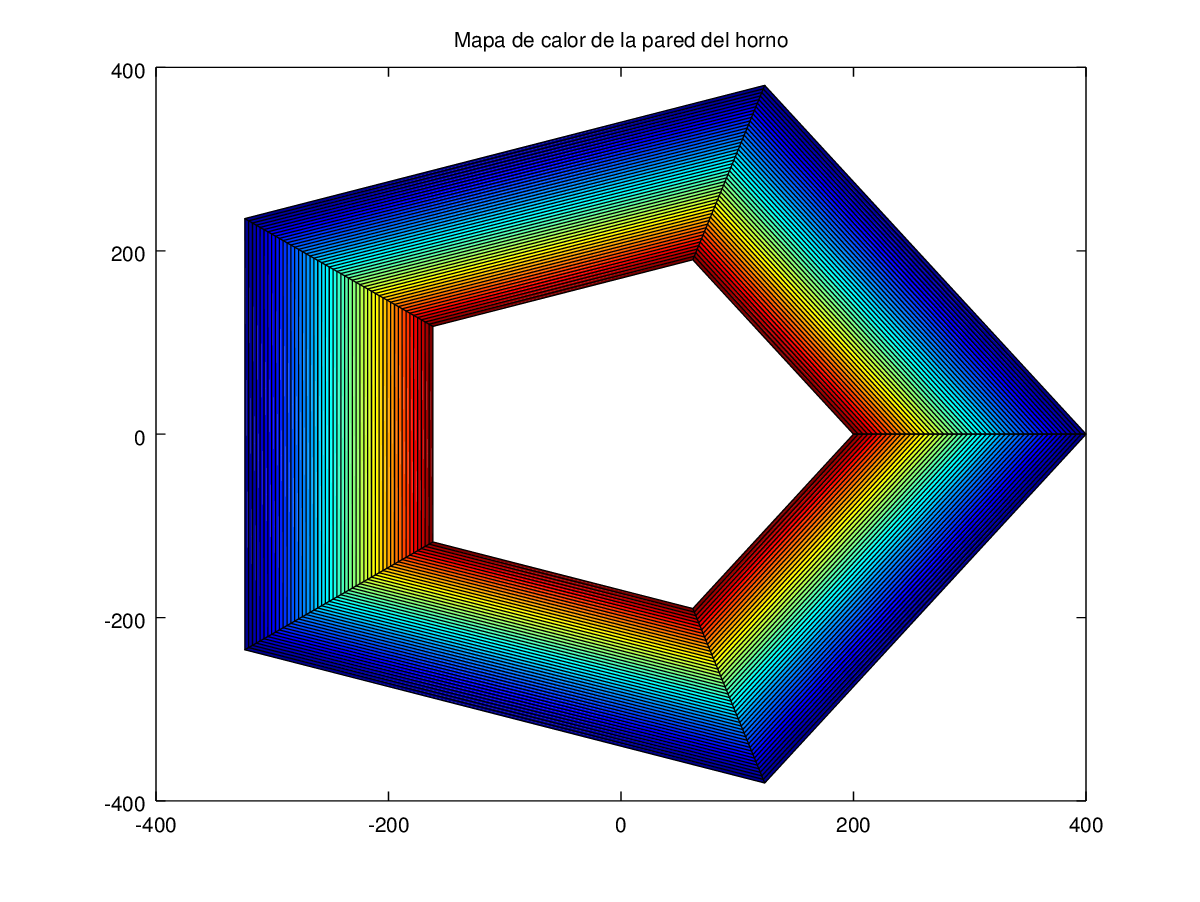
\includegraphics[scale=0.35]{experimentos1a_1b/evolucion_posicion_isoterma_temperatura/variacion_angulos_radio_fijo_se_suaviza_isoterma/test10_050_radios_005_angulos_inst_001_heatmap.png}
		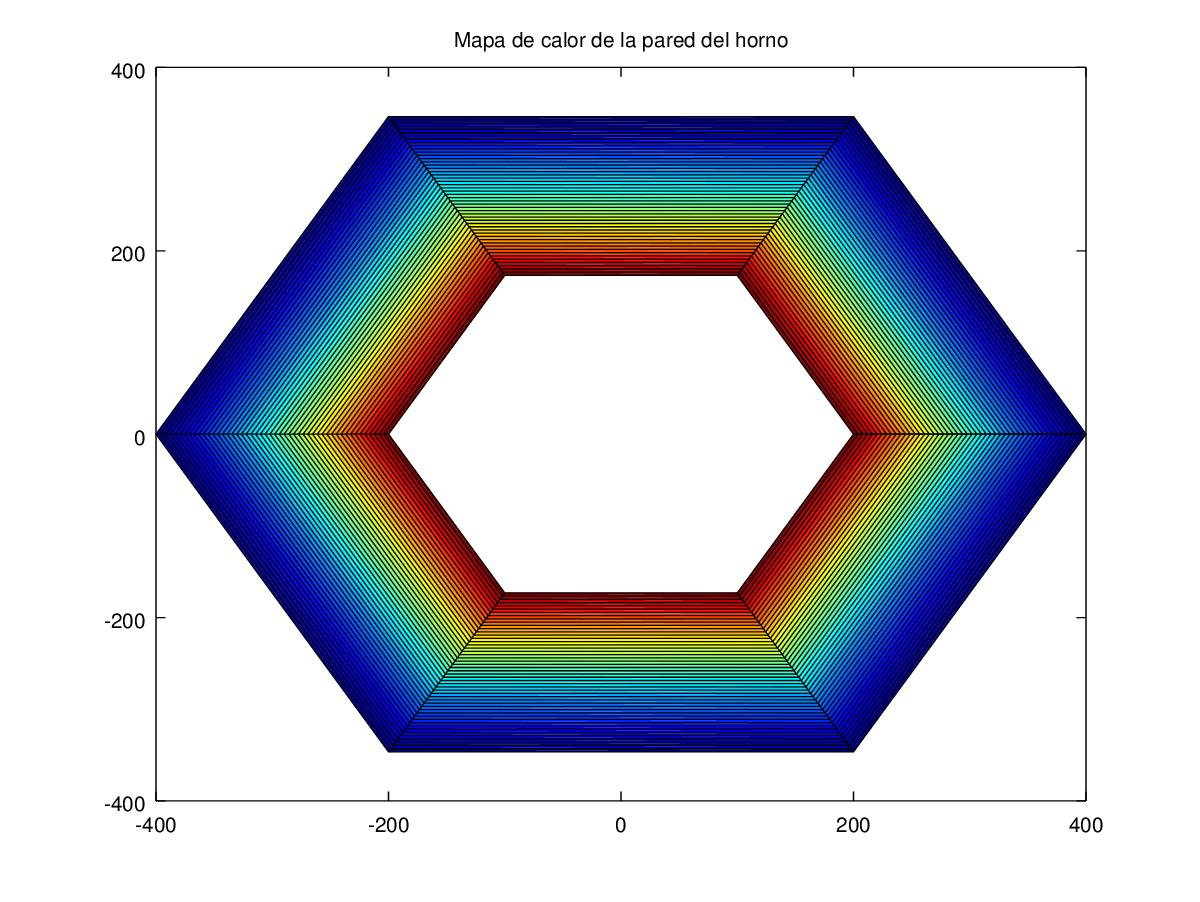
\includegraphics[scale=0.35]{experimentos1a_1b/evolucion_posicion_isoterma_temperatura/variacion_angulos_radio_fijo_se_suaviza_isoterma/test10_050_radios_006_angulos_inst_001_heatmap.png}	  	

	  	\textbf{Variación de la estimación de la isoterma entre 49 y 50 ángulos de discretización}\\
		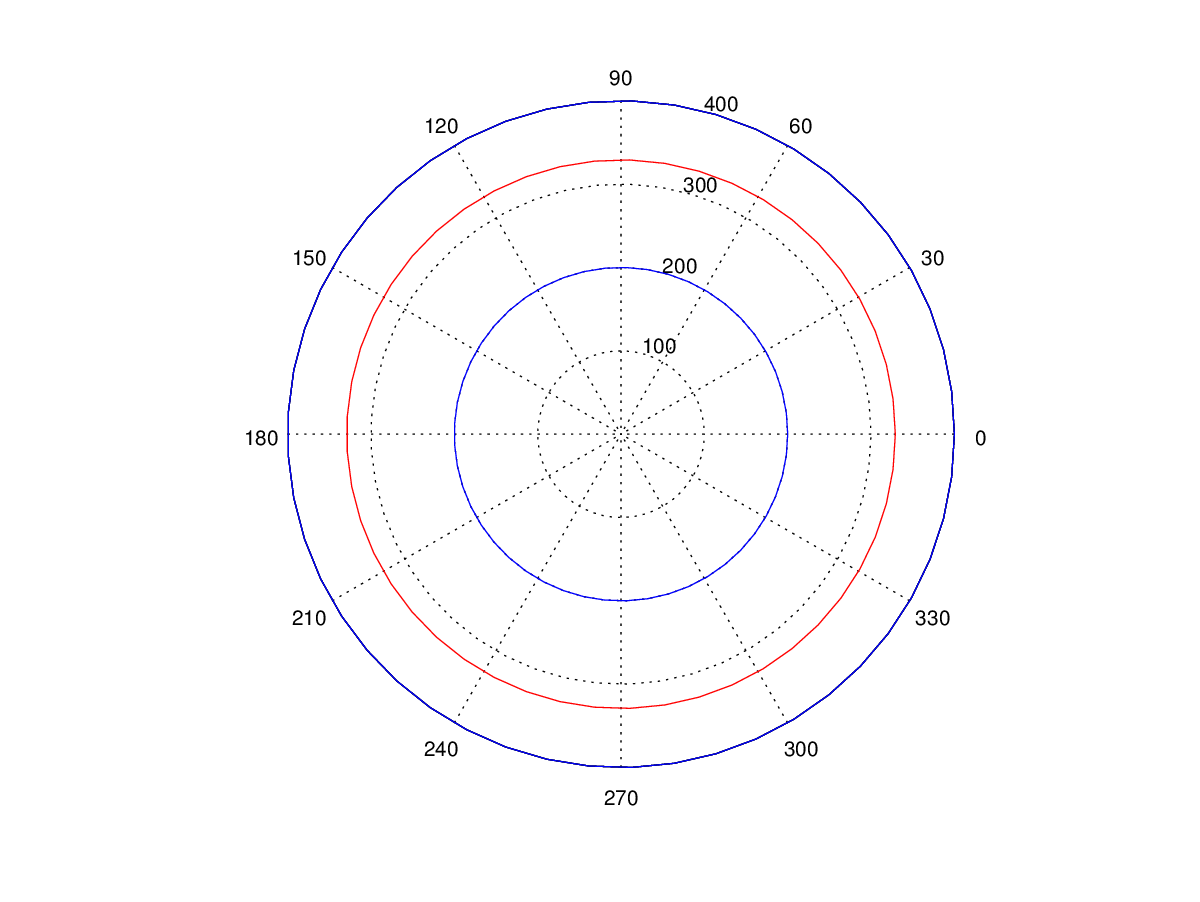
\includegraphics[scale=0.35]{experimentos1a_1b/evolucion_posicion_isoterma_temperatura/variacion_angulos_radio_fijo_se_suaviza_isoterma/test10_050_radios_049_angulos_inst_001_isomap.png}
		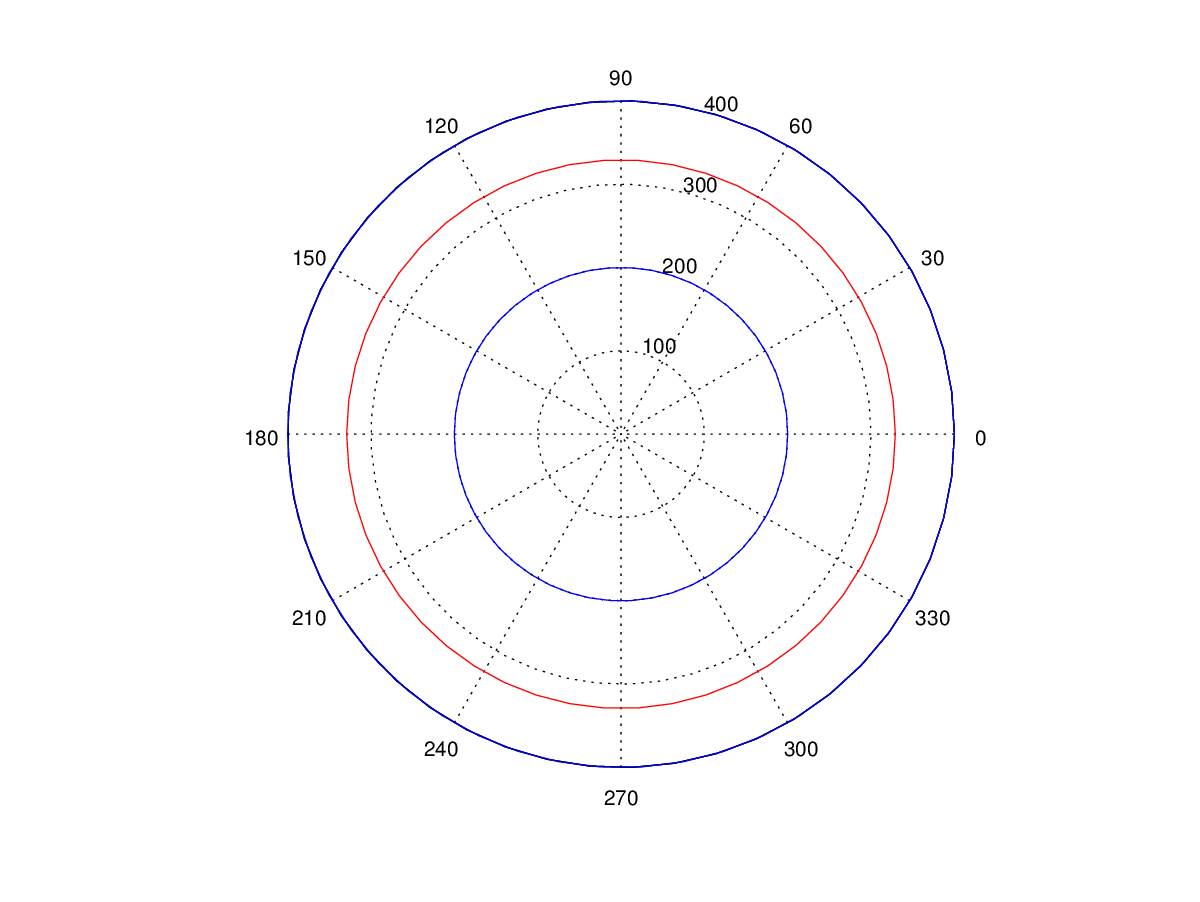
\includegraphics[scale=0.35]{experimentos1a_1b/evolucion_posicion_isoterma_temperatura/variacion_angulos_radio_fijo_se_suaviza_isoterma/test10_050_radios_050_angulos_inst_001_isomap.png}

		\textbf{Variación de la temperatura entre 49 y 50 ángulos de discretización}\\
	  	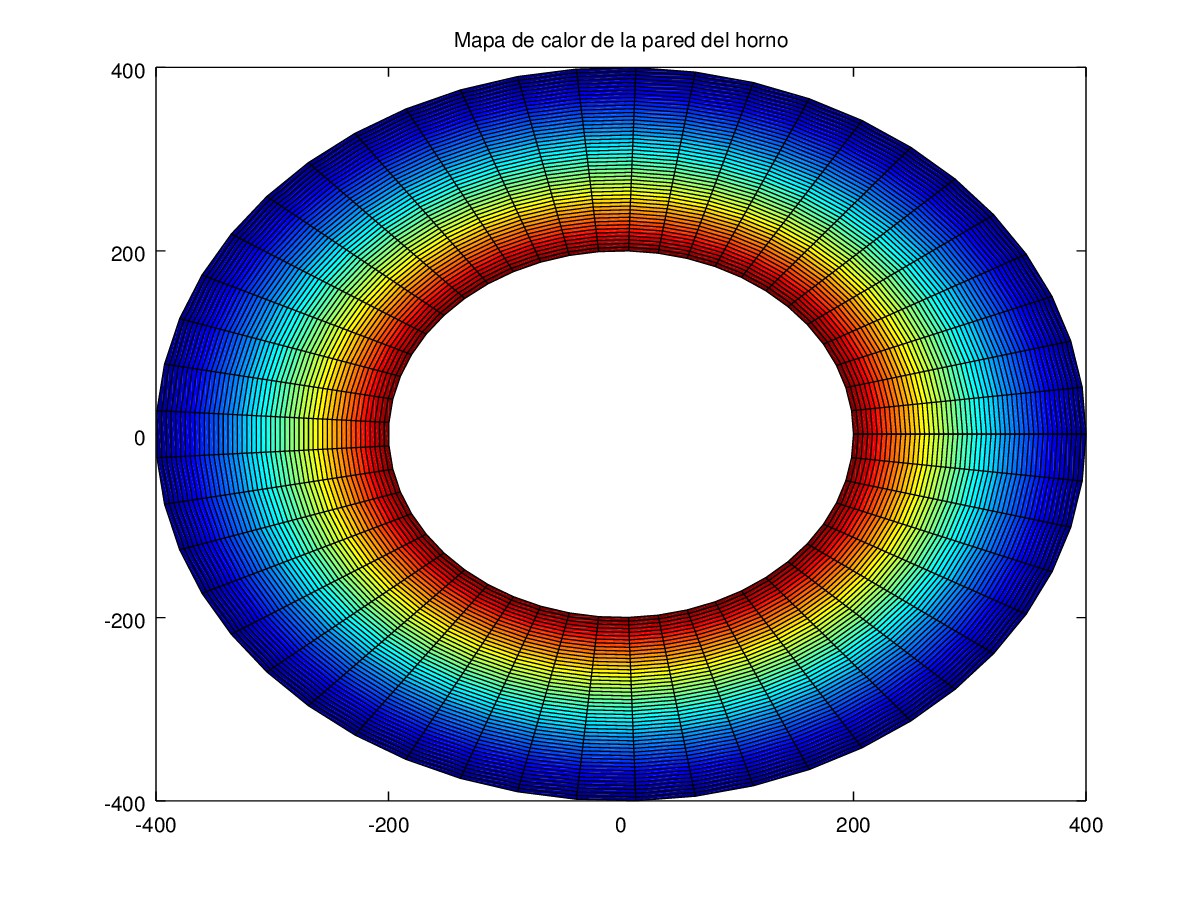
\includegraphics[scale=0.35]{experimentos1a_1b/evolucion_posicion_isoterma_temperatura/variacion_angulos_radio_fijo_se_suaviza_isoterma/test10_050_radios_049_angulos_inst_001_heatmap.png}
		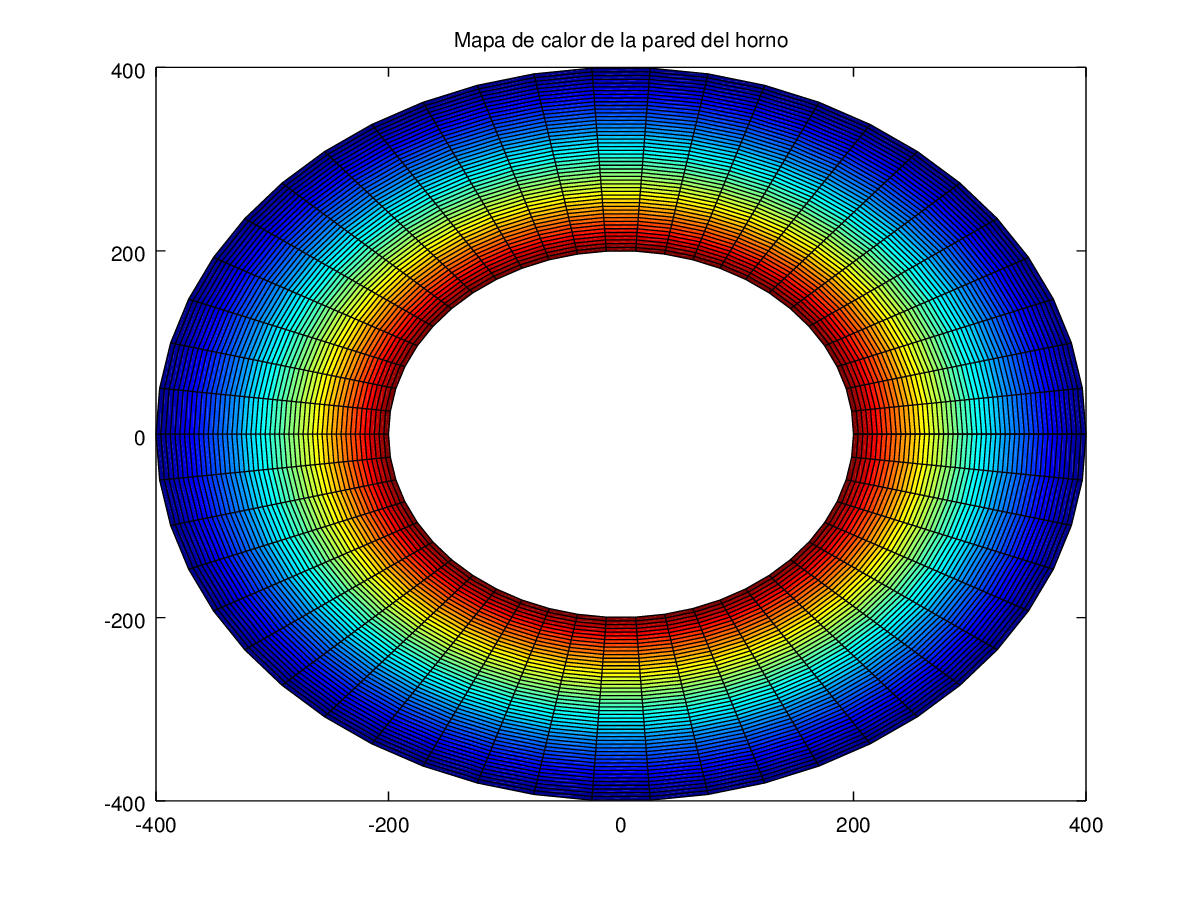
\includegraphics[scale=0.35]{experimentos1a_1b/evolucion_posicion_isoterma_temperatura/variacion_angulos_radio_fijo_se_suaviza_isoterma/test10_050_radios_050_angulos_inst_001_heatmap.png}

\vspace{0.5cm}

Aquí el radio es el mismo, pero se gana en precisión al tener más ángulos por no tener que linealizar la posición de la isoterma angularmente. Nuevamente, la posición entre dos tests consecutivos se estabiliza al aumentar la cantidad de ángulos. Tambien se observa que al cambiar el $\Delta_\theta$ los ángulos entre tests consecutivos no son los mismos.

	\item \begin{itemize}
						\item \textbf{Temperaturas internas y externas:} constantes, 100 y 1500. Esto es para que tenga la misma solución cada test del experimento.
						\item \textbf{Radio interno:} 200
						\item \textbf{Radio externo:} 400
						\item \textbf{Cantidad radios:} $[15\dots60]$
						\item \textbf{Cantidad ángulos:} $[15\dots60]$
						\item \textbf{Isoterma buscada:} 500
					\end{itemize}
	Se adjunta con el trabajo práctico un video que expone la evolución del sistema mientras se incrementa la cantidad de radios. Expondremos estáticamente algunos frames, pero es conveniente ver el video primero. Se encuentra en la misma carpeta que el pdf. (variación\_doble\_isomap.mp4, variación\_doble\_heatmap.mp4).

	\vspace{0.5cm}
	  	\textbf{Variación de la estimación de la isoterma entre 15 y 16 radios, ángulos de discretización}\\
		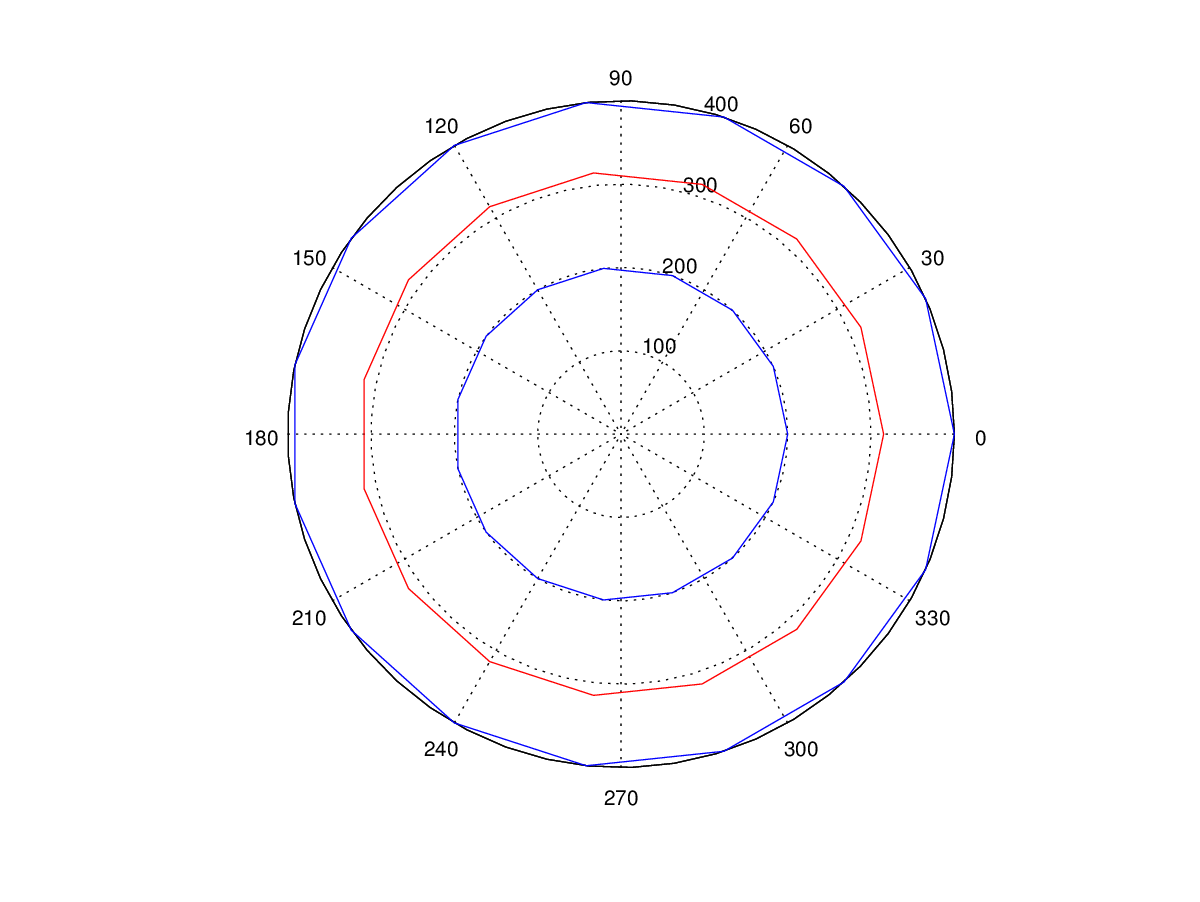
\includegraphics[scale=0.35]{experimentos1a_1b/evolucion_posicion_isoterma_temperatura/variacion_radios_angulos_se_reduce_diferencia_radial/test11_testord_001_inst_001_isomap.png}
		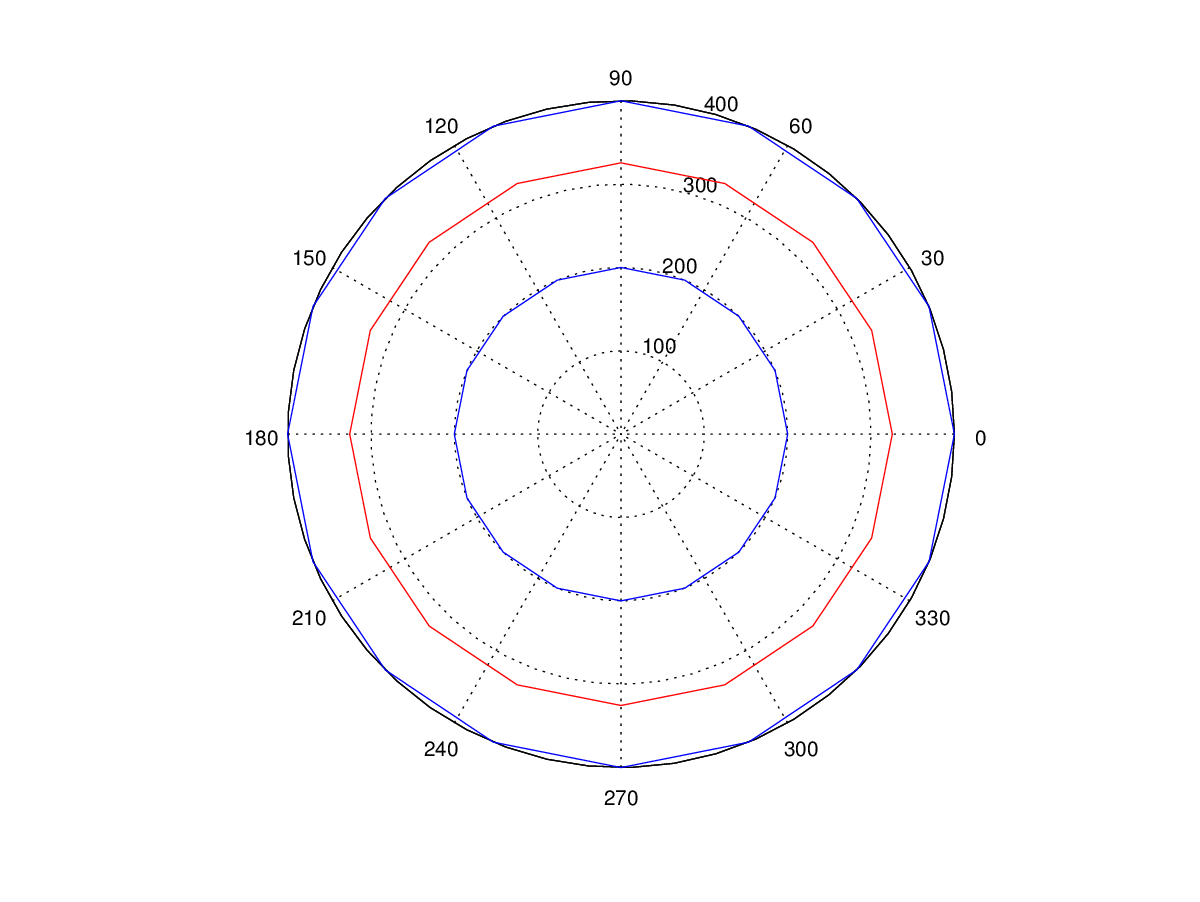
\includegraphics[scale=0.35]{experimentos1a_1b/evolucion_posicion_isoterma_temperatura/variacion_radios_angulos_se_reduce_diferencia_radial/test11_testord_002_inst_001_isomap.png}

	  	\textbf{Variación de la temperatura entre 59 y 60 radios, ángulos de discretización}\\
	  	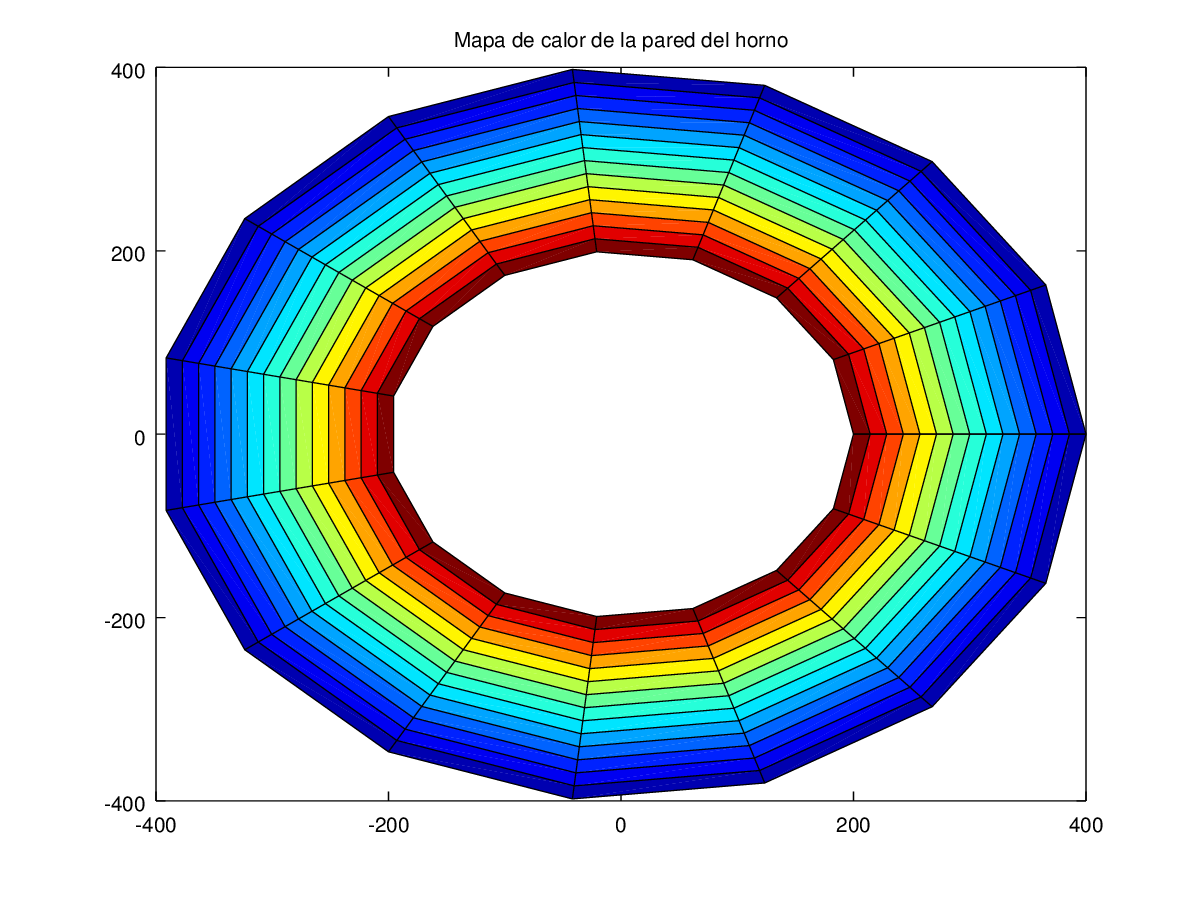
\includegraphics[scale=0.35]{experimentos1a_1b/evolucion_posicion_isoterma_temperatura/variacion_radios_angulos_se_reduce_diferencia_radial/test11_testord_001_inst_001_heatmap.png}
		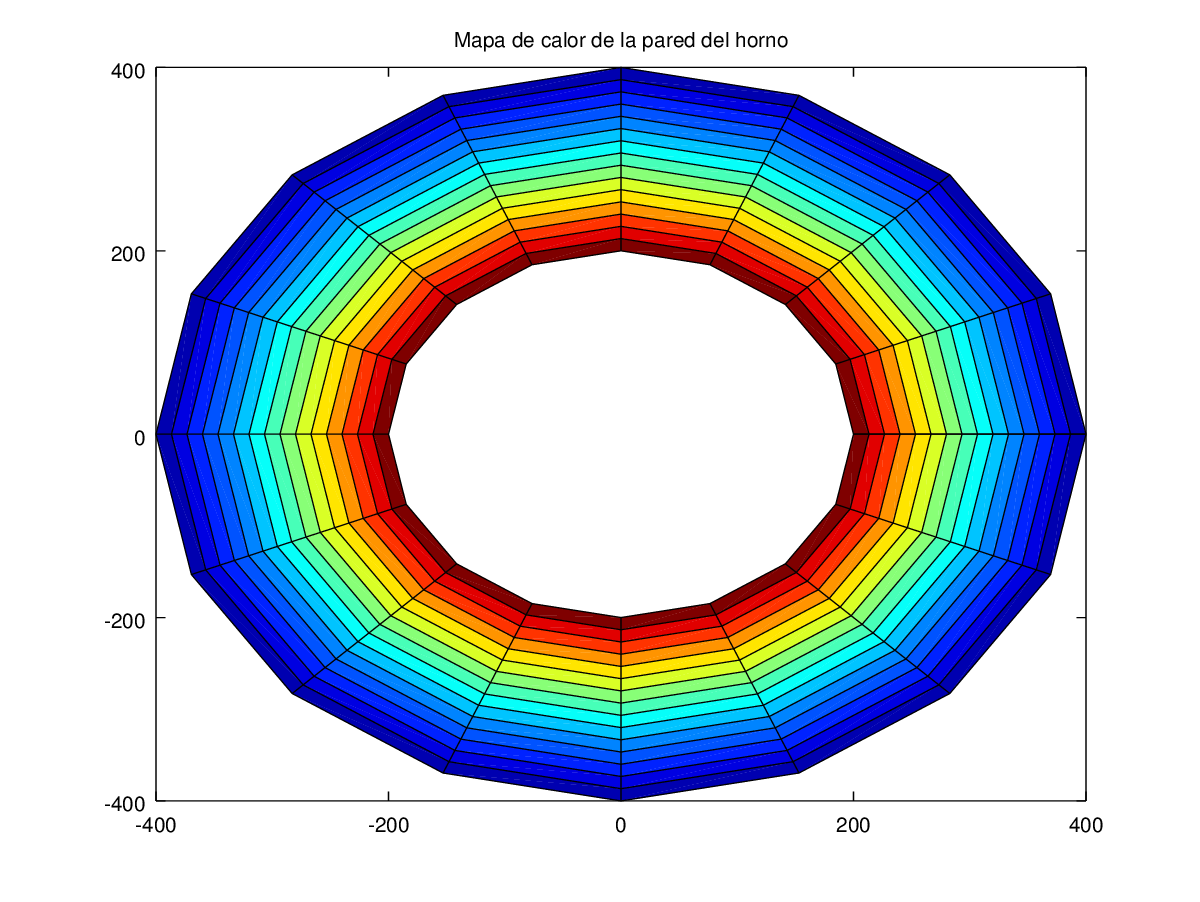
\includegraphics[scale=0.35]{experimentos1a_1b/evolucion_posicion_isoterma_temperatura/variacion_radios_angulos_se_reduce_diferencia_radial/test11_testord_002_inst_001_heatmap.png}

	  	\textbf{Variación de la estimación de la isoterma entre 15 y 16 radios, ángulos de discretización}\\
		\includegraphics[scale=0.35]{experimentos1a_1b/evolucion_posicion_isoterma_temperatura/variacion_radios_angulos_se_reduce_diferencia_radial/test11_testord_045_inst_001_isomap.png}
		\includegraphics[scale=0.35]{experimentos1a_1b/evolucion_posicion_isoterma_temperatura/variacion_radios_angulos_se_reduce_diferencia_radial/test11_testord_046_inst_001_isomap.png}

		\textbf{Variación de la temperatura entre 59 y 60 radios, ángulos de discretización}\\
	  	\includegraphics[scale=0.35]{experimentos1a_1b/evolucion_posicion_isoterma_temperatura/variacion_radios_angulos_se_reduce_diferencia_radial/test11_testord_045_inst_001_heatmap.png}
		\includegraphics[scale=0.35]{experimentos1a_1b/evolucion_posicion_isoterma_temperatura/variacion_radios_angulos_se_reduce_diferencia_radial/test11_testord_046_inst_001_heatmap.png}
\FloatBarrier
\vspace{0.5cm}

En este último ejemplo ocurren ambos fenomenos al mismo tiempo, hay una variación radial menor a medida que crecen los radios y la curva se suaviza al aumentar los ángulos.

\end{enumerate}

\vspace{0.5cm}

Efectivamente, podemos concluir que mientras más fina sea la discretización, se obtendrán resultados más \texttt{estables y confiables} acerca de la estimación. Uno de los motivos es porque habrá menos puntos para interpolar en la posición de la isoterma y el otro porque se tiene más informacion de la temperatura de la pared del horno.

\subsubsection{Estimación de estabilidad de la pared del horno}

Se presentarán a continuación los resultados de la estimacion de la estabilidad del horno. Para varios tipos de discretizaciones donde la cantidad de ángulos y radios son iguales, se evalua el cambio de posicion de la isoterma a medida que va aumentando la temperatura externa entre 100 y 300 grados, de a 2 grados por paso. Dado que las temperaturas son constantes, el máximo y el promedio coinciden como métricas de posicionamiento relativo de la isoterma.

\begin{figure}[h]
\centering

\includegraphics[scale=0.3]{experimentos1a_1b/evolucion_estimacion_seguridad_isoterma/variacion_25.png}
\includegraphics[scale=0.3]{experimentos1a_1b/evolucion_estimacion_seguridad_isoterma/variacion_50.png}	

\caption{Cantidad de radios y ángulos: 25(Izq) 50(Der)}
\end{figure}

\begin{figure}[h]
\centering

\includegraphics[scale=0.3]{experimentos1a_1b/evolucion_estimacion_seguridad_isoterma/variacion_75.png}
\includegraphics[scale=0.3]{experimentos1a_1b/evolucion_estimacion_seguridad_isoterma/variacion_100.png}	

\caption{Cantidad de radios y ángulos: 75(Izq) 100(Der)}
\end{figure}

\begin{figure}[h]
\centering

\includegraphics[scale=0.5]{experimentos1a_1b/evolucion_estimacion_seguridad_isoterma/variacion_125.png}

\caption{Cantidad de radios y ángulos: 125}
\end{figure}

\begin{figure}[h]
\centering

\includegraphics[scale=0.5]{experimentos1a_1b/evolucion_estimacion_seguridad_isoterma/variacion_30a_200r.png}
\caption{Cantidad de radios 200 - ángulos: 30}

\includegraphics[scale=0.5]{experimentos1a_1b/evolucion_estimacion_seguridad_isoterma/variacion_5a_500r.png}
\caption{Cantidad de radios 500 - ángulos: 5}
\end{figure}
\FloatBarrier

Los gráficos son un poco mas extraños de lo esperado. Se observa que, para cualquier discretizacion fija, al aumentar la temperatura externa, la isoterma tiende a acercarse a la pared externa. Esto es lo esperable, el método propuesto para determinar la seguridad de la isoterma consiste en fijar un umbral sobre la posicion relativa máxima o promedio. Lo que se observa como raro es la curva \texttt{dentada} a medida que crecen las temperaturas. Veamos además que estos \texttt{dientes} disminuyen su intensidad a medida que se van agregando radios a la discretizacion. 

\begin{proposition} 
	Bajo que las temperaturas internas y externas constantes, la posicion radial de la isoterma es la misma en todo ángulo.	
\end{proposition}

Dada esta última proposición, podemos hacer experimentos con muy pocos ángulos y muchos radios que nos den pauta de que ocurre con esos \texttt{dientes} en los gráficos. \\
Se puede observar en las figuras con 200 y 500 radios, que a medida que $m\to\infty$ , la curva se suaviza. Lo cual nos hace pensar, que la estimacion lineal de la isoterma esta generando esta distorsión.

\vspace{0.5cm}

Consideremos nuevamente $\hat{g_{\theta_i}}$: la función \textbf{discreta de aproximaciones} de temperatura de un ángulo i. A medida que las temperaturas aumentan linealmente, los 2 puntos $x$ y $x'$ que acotan la isoterma buscada en dicha función van aumentando tambien, generando que la estimacion del punto intermedio entre ellos decrezca. Creemos que cuando esos 2 puntos dejan se encerrar el valor buscado, es que se produce el \texttt{salto} en el gráfico.

\begin{proposition}
	El método de umbral de seguridad es inconsistente tomando la distancia máxima relativa o distancia promedio relativa a la pared exterior.
\end{proposition}

En los resultados anteriores y en el gráfico presentado en el primer experimento de ubicacion de la isoterma (convergencia radial de la isoterma). Se puede observar claramente, que trazando una recta horizontal en algún punto del eje Y, la determinación de colapso no es consistente. Es decir, existen $t_1 < t_2 < t_3$ temperaturas crecientes donde tanto la posicion máxima relativa o la posicion promedio relativa, indican peligro de colapso para $t_2$ pero no para $t_1$ ni $t_3$. Sin embargo, cuando $m\to\infty$ esto tiende a ser \texttt{menos inconsistente}.

\subsubsection{Análisis de la interpolacion lineal de la curva de temperatura}

Dados los resultados de la sección anterior, nos interesó saber un poco mas la forma de la funcion de temperatura sobre un ángulo fijo $\hat{g_{\theta_i}}$. 
Variamos un poco la cantidad de radios, y graficamos la función obtenida de los puntos de la discretización en una dirección fija y un fitteo lineal.
El resultado de los gráficos muestra que la temperatura no se disipa linealmente entre el interior y el exterior del horno. Dado que nosotros aproximamos linealmente la posicion radial de la isoterma 500 \textbf{entre los 2 puntos mas cercanos}, tendremos un error en cada \texttt{cambio de puntos} para la aproximacion.\\

Esto fortalece nuestra hipótesis de la sección anterior de que la forma de diente de sierra de los gráficos podía deberse a la interpolacion de algo no lineal, mediante una recta en puntos consecutivos.

\begin{figure}[h]
\centering
\includegraphics[scale=0.34]{funcion_temp_50_radios_ti_1500_te_102.png}
\includegraphics[scale=0.34]{funcion_temp_50_radios_ti_1500_te_202.png}
\caption{Distintas temperaturas externas - Cantidad de radios: 50}
\end{figure}
\FloatBarrier

\begin{figure}[h]
\centering
\includegraphics[scale=0.34]{funcion_temp_75_radios_ti_1500_te_102.png}
\includegraphics[scale=0.34]{funcion_temp_75_radios_ti_1500_te_202.png}
\caption{Distintas temperaturas externas - Cantidad de radios: 75}
\end{figure}
\FloatBarrier

\begin{figure}[h]
\centering
\includegraphics[scale=0.34]{funcion_temp_150_radios_ti_1500_te_102.png}
\includegraphics[scale=0.34]{funcion_temp_500_radios_ti_1500_te_102.png}
\caption{Cantidad de radios: 150(izq) , 500(der)}
\end{figure}
\FloatBarrier

\begin{figure}[h]
\centering
\includegraphics[scale=0.8]{efecto_interpolacion_lineal.png}
\caption{Esquema aproximado: Efecto interpolacion lineal entre puntos de algo no lineal}
\label{fig:aprox}
\end{figure}
\FloatBarrier

En la figura \ref{fig:aprox} se ve lo que podría estar ocurriendo al aproximar linealmente 2 puntos de una curva que realmente no es lineal. La recta entre dos puntos queda por encima de la curva real, luego, si se quiere hallar el $x$ tal que $g(x) = \alpha$ , la aproximación falla por un $\epsilon$ que depende de la concavidad de la curva respecto a la recta. A medida que se van agregando radios a la discretizacion, la distancia entre los puntos que se aproximan disminuye, disminuyendo el error cometido al estimar. 


%    \FloatBarrier

%\newpage
%\section{Discusi\'on}
%    % TODO
Se incluira aqu un analisis de los resultados obtenidos en la seccion anterior (se analizara
su  validez,  coherencia,  etc.).   Deben  analizarse  como  mnimo  los tems  pedidos  en  el
enunciado.  No es aceptable decir que los resultados fueron los esperados", sin hacer
clara referencia a la teora a la cual se ajustan.  Ademas, se deben mencionar los resul-
tados interesantes y los casos patologicos" encontrados.


%    \FloatBarrier

% An example of a floating figure using the graphicx package.
% Note that \label must occur AFTER (or within) \caption.
% For figures, \caption should occur after the \includegraphics.
% Note that IEEEtran v1.7 and later has special internal code that
% is designed to preserve the operation of \label within \caption
% even when the captionsoff option is in effect. However, because
% of issues like this, it may be the safest practice to put all your
% \label just after \caption rather than within \caption{}.
%
% Reminder: the "draftcls" or "draftclsnofoot", not "draft", class
% option should be used if it is desired that the figures are to be
% displayed while in draft mode.
%
%\begin{figure}[!t]
%\centering
%\includegraphics[width=2.5in]{myfigure}
% where an .eps filename suffix will be assumed under latex,
% and a .pdf suffix will be assumed for pdflatex; or what has been declared
% via \DeclareGraphicsExtensions.
%\caption{Simulation Results.}
%\label{fig_sim}
%\end{figure}

% Note that IEEE typically puts floats only at the top, even when this
% results in a large percentage of a column being occupied by floats.
% However, the Computer Society has been known to put floats at the bottom.


% An example of a double column floating figure using two subfigures.
% (The subfig.sty package must be loaded for this to work.)
% The subfigure \label commands are set within each subfloat command,
% and the \label for the overall figure must come after \caption.
% \hfil is used as a separator to get equal spacing.
% Watch out that the combined width of all the subfigures on a
% line do not exceed the text width or a line break will occur.
%
%\begin{figure*}[!t]
%\centering
%\subfloat[Case I]{\includegraphics[width=2.5in]{box}%
%\label{fig_first_case}}
%\hfil
%\subfloat[Case II]{\includegraphics[width=2.5in]{box}%
%\label{fig_second_case}}
%\caption{Simulation results.}
%\label{fig_sim}
%\end{figure*}
%
% Note that often IEEE papers with subfigures do not employ subfigure
% captions (using the optional argument to \subfloat[]), but instead will
% reference/describe all of them (a), (b), etc., within the main caption.


% An example of a floating table. Note that, for IEEE style tables, the
% \caption command should come BEFORE the table. Table text will default to
% \footnotesize as IEEE normally uses this smaller font for tables.
% The \label must come after \caption as always.
%
%\begin{table}[!t]
%% increase table row spacing, adjust to taste
%\renewcommand{\arraystretch}{1.3}
% if using array.sty, it might be a good idea to tweak the value of
% \extrarowheight as needed to properly center the text within the cells
%\caption{An Example of a Table}
%\label{table_example}
%\centering
%% Some packages, such as MDW tools, offer better commands for making tables
%% than the plain LaTeX2e tabular which is used here.
%\begin{tabular}{|c||c|}
%\hline
%One & Two\\
%\hline
%Three & Four\\
%\hline
%\end{tabular}
%\end{table}


% Note that IEEE does not put floats in the very first column - or typically
% anywhere on the first page for that matter. Also, in-text middle ("here")
% positioning is not used. Most IEEE journals use top floats exclusively.
% However, Computer Society journals sometimes do use bottom floats - bear
% this in mind when choosing appropriate optional arguments for the
% figure/table environments.
% Note that, LaTeX2e, unlike IEEE journals, places footnotes above bottom
% floats. This can be corrected via the \fnbelowfloat command of the
% stfloats package.



%\section{Conclusion}
%The conclusion goes here.

\newpage
\section{Conclusiones}\label{sec:conclusiones}
    %!TEX root = informe.tex
\IEEEPARstart{A}{} lo largo de este trabajo atacamos el problema de generar frames artificiales para un video, intentando lograr que se ajusten al original hasta el punto -ideal- de que el ojo humano no detecte la diferencia con un video filmado en alta frecuencia.

Como primera conclusión al respecto podemos decir que no logramos dicho objetivo ideal: de nuestras observaciones descubrimos fácilmente que, al menos para los tres métodos implementados, los resultados ``no engañan a nadie''. Todos los métodos presentan o bien \emph{lag} o bien \emph{fantasmeo}, perturbando la sensación de fluidez y alterando el realismo percibido del video.

Más allá de ese análisis cualitativo, pudimos observar que atacar el problema de forma \emph{naïve} (el método que llamamos ``Vecino más cercano'') produce resultados con error matemático más reducido aunque visualmente pareciera ser el peor método, pudiendo obtenerse resultados visualmente más agradables con métodos más inteligentes como interpolación mediante poliniomios.

También concluimos que, visto como método de compresión, los resultados son pobres. En la actualidad existen métodos que, sin utilizar mucho más espacio, generan prácticamente nulos \emph{artifacts} y no pierden información de cuadros completos.


% if have a single appendix:
%\appendix[Proof of the Zonklar Equations]
% or
%\appendix  % for no appendix heading
% do not use \section anymore after \appendix, only \section*
% is possibly needed

% use appendices with more than one appendix
% then use \section to start each appendix
% you must declare a \section before using any
% \subsection or using \label (\appendices by itself
% starts a section numbered zero.)
%


%\appendices
%\section{Proof of the First Zonklar Equation}
%Appendix one text goes here.

% you can choose not to have a title for an appendix
% if you want by leaving the argument blank
%\section{}
%Appendix two text goes here.

\newpage
\appendices
\section{Enunciado del Trabajo Pr\'actico}\label{sec:enunciado}
    %\documentclass[11pt, a4paper]{article}
%\usepackage[spanish]{babel}
%\usepackage{a4wide}
%\usepackage{amsfonts}
%\usepackage{graphicx}
%\usepackage{verbatim}
%\usepackage{todonotes}
%\usepackage{amsmath}
%\usepackage{url}

%\usepackage{tikz}
%\usetikzlibrary{decorations.markings,arrows}

\parindent = 0 pt
\parskip = 5 pt

%\newcommand{\real}{\hbox{\bf R}}

%\begin{document}
\begin{center}
\begin{tabular}{r|cr}
 \begin{tabular}{c}
{\large\bf\textsf{\ M\'etodos Num\'ericos\ }}\\ 
Segundo Cuatrimestre 2015\\
{\bf Trabajo Pr\'actico 2}\\
\end{tabular} &
\begin{tabular}{@{} p{1.6cm} @{}}
\includegraphics[width=1.6cm]{img/logodpt.jpg}
\end{tabular} &
\begin{tabular}{l @{}}
 \emph{Departamento de Computaci\'on} \\
 \emph{Facultad de Ciencias Exactas y Naturales} \\
 \emph{Universidad de Buenos Aires} \\
\end{tabular} 
\end{tabular}
\vskip 10pt
\textbf{\Large \emph{Ohhh solo tiran $\pi$-edras...}}
\end{center}

\vskip 10pt
\hrule
\vskip 5pt

\noindent\textbf{Contexto y motivaci\'on}
\vskip 5pt

 
%\vskip 5pt
%\noindent\textbf{Contexto}
%\vskip 5pt

A partir de la evoluci\'on de Internet durante la d\'ecada de 1990, el desarrollo de motores de b\'usqueda se ha convertido en uno de los aspectos 
centrales para su efectiva utilizaci\'on. Hoy en d\'ia, sitios como Yahoo, Google y Bing ofrecen distintas alternativas para realizar b\'usquedas 
complejas dentro de un red que contiene miles de millones de p\'aginas web. 

En sus comienzos, una de las caracter\'isticas que distingui\'o a Google respecto de los motores de b\'usqueda de la \'epoca fue la calidad de los 
resultados obtenidos, mostrando al usuario p\'aginas relevantes a la b\'usqueda realizada. El esquema general de los or\'igenes de este motor de 
b\'usqueda es brevemente explicado en Brin y Page \cite{Brin1998}, donde se mencionan aspectos t\'ecnicos que van desde la etapa de obtenci\'on de
informaci\'on de las p\'aginas disponibles en la red, su almacenamiento e indexado y su posterior procesamiento, buscando ordenar cada p\'agina de 
acuerdo a su importancia relativa dentro de la red. El algoritmo utilizado para esta \'ultima etapa es denominado PageRank y es uno (no el \'unico) 
de los criterios utilizados para ponderar la importancia de los resultados de una b\'usqueda. En este trabajo nos concentraremos en el estudio y 
desarrollo del algoritmo PageRank.

Por otro lado, las competencias deportivas, en todas sus variantes y disciplinas, requieren casi inevitablemente la comparaci\'on entre competidores
mediante la confecci\'on de \emph{Tablas de Posiciones} y \emph{Rankings} en base a resultados obtenidos en un per\'iodo de tiempo determinado. 
Estos ordenamientos de equipos est\'an generalmente (aunque no siempre) basados en reglas relativamente claras y simples, como proporci\'on 
de victorias sobre partidos jugados o el cl\'asico sistema de puntajes por partidos ganados, empatados y perdidos. Sin embargo, estos m\'etodos
simples y conocidos por todos muchas veces no logran capturar la complejidad de la competencia y la comparaci\'on. Esto es particularmente
evidente en ligas donde, por ejemplo, todos los equipos no juegan la misma cantidad de veces entre s\'i.

A modo de ejemplo, la NBA y NFL representan dos ligas con fixtures de temporadas regulares con estas caracter\'isticas. Recientemente, el Torneo de 
Primera Divisi\'on de AFA se suma a este tipo de competencias, ya que la incorporaci\'on de la \emph{Fecha de Cl\'asicos} parece ser una interesante 
idea comercial, pero no tanto desde el punto de vista deportivo ya que cada equipo juega contra su \emph{cl\'asico} m\'as veces que el resto. 
Como contraparte, \'estos rankings son utilizados muchas veces como criterio de decisi\'on, como por ejemplo para determinar la participaci\'on en 
alguna competencia de nivel internacional, con lo cual la confecci\'on de los mismos constituye un elemento sensible, afectando intereses deportivos 
y econ\'omicos de gran relevancia.


\vskip 5pt
\noindent\textbf{El problema, Parte I: PageRank y p\'aginas web}
\vskip 5pt

El algoritmo PageRank se basa en la construcci\'on del siguiente modelo. Supongamos que tenemos una red con $n$ p\'aginas 
web $Web = \{1,\dots,n\}$ donde
el objetivo es asignar a cada una de ellas un puntaje que determine la importancia relativa de la misma respecto de las
dem\'as. Para modelar las relaciones entre ellas, definimos la \emph{matriz de conectividad} $W \in \{0,1\}^{n \times n}$ 
de forma tal que $w_{ij} = 1$ si la p\'agina $j$ tiene un link a la p\'agina $i$, y $w_{ij} = 0$ en caso contrario. 
Adem\'as, ignoramos los \emph{autolinks}, es decir, links de una p\'agina a s\'i misma, definiendo $w_{ii} = 0$. Tomando 
esta matriz, definimos el grado de la p\'agina $j$, $n_j$, como la cantidad de links salientes hacia otras p\'aginas 
de la red, donde $n_j = \sum_{i = 1}^n w_{ij}$. Adem\'as, notamos con $x_j$ al puntaje asignado a la p\'agina $j\in
Web$, que es lo que buscamos calcular.

La importancia de una p\'agina puede ser modelada de diferentes formas. Un link de la p\'agina $u \in
Web$ a la p\'agina $v \in Web$ puede ser visto como que $v$ es una p\'agina importante. Sin embargo, no queremos que una
p\'agina obtenga mayor importancia simplemente porque es apuntada desde muchas p\'aginas. 
Una forma de limitar esto es ponderar los links utilizando la importancia de la p\'agina de origen. En otras palabras,
pocos links de p\'aginas importantes pueden valer m\'as que muchos links de p\'aginas poco importantes. En particular,
consideramos que la importancia de la p\'agina $v$ obtenida mediante el link de la p\'agina $u$ es proporcional a la 
importancia de la p\'agina $u$ e inversamente proporcional al grado de $u$. Si la p\'agina $u$ contiene $n_u$ links,
uno de los cuales apunta a la p\'agina $v$, entonces el aporte de ese link a la p\'agina $v$ ser\'a $x_u/n_u$. Luego,
sea $L_k \subseteq Web$ el conjunto de p\'aginas que tienen un link a la p\'agina $k$. Para cada p\'agina pedimos que
\begin{eqnarray}
x_k = \sum_{j \in L_k} \frac{x_j}{n_j},~~~~k = 1,\dots,n. \label{eq:basicmodel}
\end{eqnarray}
Definimos $P \in  \mathbb{R}^{n \times n}$ tal que $p_{ij} = 1/n_j$ si $w_{ij} = 1$, y $p_{ij} = 0$ en caso contrario. Luego,
el modelo planteado en (\ref{eq:basicmodel}) es equivalente a encontrar un $x\in \mathbb{R}^n$ tal que $Px = x$, es
decir, encontrar (suponiendo que existe) un autovector asociado al autovalor 1 de una matriz cuadrada, tal que $x_i \ge
0$ y $\sum_{i = 1}^n x_i = 1$. En
Bryan y Leise \cite{Bryan2006} y Kamvar et al. \cite[Secci\'on 1]{Kamvar2003} se analizan ciertas condiciones que debe
cumplir la red de p\'aginas para garantizar la existencia de este autovector.

Una interpretaci\'on equivalente para el problema es considerar al \emph{navegante aleatorio}. \'Este empieza en una
p\'agina cualquiera del conjunto, y luego en cada p\'agina $j$ que visita sigue navegando a trav\'es de sus links,
eligiendo el mismo con probabilidad $1/n_j$. Una situaci\'on particular se da cuando la p\'agina no tiene links salientes. En
ese caso, consideramos que el navegante aleatorio pasa a cualquiera de las p\'agina de la red con probabilidad $1/n$.
Para representar esta situaci\'on, definimos $v \in \mathbb{R}^{n \times n}$, con $v_i = 1/n$ y $d \in \{0,1\}^{n}$ donde 
$d_i = 1$ si $n_i = 0$, y $d_i = 0$ en caso contrario. La nueva matriz de transici\'on es 
\begin{eqnarray*}
D & = & v d^t \\
P_1 & = & P + D.
\end{eqnarray*}
Adem\'as, consideraremos el caso de que el navegante aleatorio, dado que se encuentra en la p\'agina $j$, decida visitar
una p\'agina cualquiera del conjunto, independientemente de si esta se encuentra o no referenciada por $j$ (fen\'omeno
conocido como \emph{teletransportaci\'on}). Para ello, consideramos que esta decisi\'on se toma con una probabilidad
$c \ge 0$, y podemos incluirlo al modelo de la siguiente forma:
\begin{eqnarray*}
E & = & v \bar{1}^t \\
P_2 & = & cP_1 + (1-c)E,
\end{eqnarray*}
\noindent donde $\bar{1} \in \mathbb{R}^n$ es un vector tal que todas sus componentes valen 1. La matriz resultante
$P_2$ corresponde a un enriquecimiento del modelo formulado en (\ref{eq:basicmodel}). Probabil\'isticamente, la
componente $x_j$ del vector soluci\'on (normalizado) del sistema $P_2 x = x$ representa la proporci\'on del tiempo que,
en el largo plazo, el navegante aleatorio pasa en la p\'agina $j \in Web$. Denotaremos con $\pi$ al vector soluci\'on 
de la ecuaci\'on $P_2 x = x$, que es com\'unmente denominado \emph{estado estacionario}.

En particular, $P_2$ corresponde a una
matriz \emph{estoc\'astica por columnas} que cumple las hip\'otesis planteadas en Bryan y Leise \cite{Bryan2006} y
Kamvar et al. \cite{Kamvar2003}, tal que $P_2$ tiene un autovector asociado al autovalor 1, los dem\'as autovalores de
la matriz cumplen $1 = \lambda_1 > |\lambda_2| \ge \dots \ge |\lambda_n|$ y, adem\'as, la dimensi\'on
del autoespacio asociado al autovalor $\lambda_1$ es 1. Luego, $\pi$ puede ser calculada
de forma est\'andar utilizando el m\'etodo de la potencia.

Una vez calculado el ranking, se retorna al usuario las $t$ p\'aginas con mayor puntaje.

\vskip 5pt
\noindent\textbf{El problema, Parte II: PageRank y ligas deportivas}
\vskip 5pt

Existen en la literatura distintos enfoques para abordar el problema de determinar el \emph{ranking} de equipos de una competencia en
base a los resultados de un conjunto de partidos. En Govan et al. \cite{Govan2008} se hace una breve rese\~na de dos ellos, y los autores
proponen un nuevo m\'etodo basado en el algoritmo PageRank que denominan GeM\footnote{Aunque no se especifica, asumimos que el nombre se
debe a las iniciales de los autores.}. Conceptualmente, el m\'etodo GeM representa la temporada como un red (grafo) donde las p\'aginas web
representan a los equipos, y existe un link (que tiene un valor, llamado peso, asociado) entre dos equipos que los relaciona modelando los resultados de los posibles
enfrentamientos entre ellos. En base a este modelo, Govan et al. \cite{Govan2008} proponen calcular el ranking de la misma forma que en el 
caso de las p\'aginas web.

En su versi\'on b\'asica, que es la que consideraremos en el presente trabajo, el m\'etodo GeM (ver, e.g., \cite[Secci\'on GeM Ranking Method]{Govan2008}) 
es el siguiente\footnote{Notar que en art\'iculo, Govan et al. \cite{Govan2008} lo definen sobre la traspuesta. La definici\'on y las cuentas son
equivalentes, simplemente se modifica para mantener la consistencia a lo largo del enunciado.}:
\begin{enumerate}
\item La temporada se representa mediante un grafo donde cada equipo representa un nodo y existe un link de $i$ a $j$ si el equipo $i$ perdi\'o al
menos una vez con el equipo $j$.
\item Se define la matriz $A^t \in \mathbb{R}^{n \times n}$

\begin{equation*}
A_{ji}^t = \left\{
	\begin{array}{cl}
	w_{ji} & \text{si el equipo } i \text{ perdi\'o con el equipo } j,\\
	0 & \text{en caso contrario, }\\
	\end{array} \right.
\end{equation*}

\noindent donde $w_{ji}$ es la diferencia absoluta en el marcador. En caso de que $i$ pierda m\'as de una vez con $j$, $w_{ji}$ representa la suma
acumulada de diferencias. Notar que $A^t$ es una generalizaci\'on de la matriz de conectividad $W$ definida en la secci\'on anterior.

\item Definir la matriz $H_{ji}^t \in \mathbb{R}^{n \times n}$ como
\begin{equation*}
H_{ji}^t = \left\{
	\begin{array}{cl}
	A_{ji}^t/\sum_{k = 1}^n A_{ki}^t & \text{si hay un link } i \text{ a } j,\\
	0 & \text{en caso contrario.}\\
	\end{array} \right.
\end{equation*}

\item Tomar $P = H^t$, y aplicar el m\'etodo PageRank como fue definido previamente, siendo $\pi$ la soluci\'on a la ecuaci\'on $P_2 x = x$. Notar que 
los p\'aginas sin links salientes, en este contexto se corresponden con aquellos equipos que se encuentran invictos.

\item Utilizar los puntajes obtenidos en $\pi$ para ordenar los equipos.
\end{enumerate}

En funci\'on del contexto planteado previamente, el m\'etodo GeM define una estructura que relaciona equipos dependiendo de los resultados parciales y
obtener un ranking utilizando solamente esta informaci\'on.

\vskip 5pt
\noindent\textbf{Enunciado}
\vskip 5pt

El objetivo del trabajo es experimentar en el contexto planteado utilizando el algoritmo PageRank con las variantes propuestas. A su vez, se busca
comparar los resultados obtenidos cualitativa y cuantitativamente con los algoritmos tradicionales utilizados en cada uno de los contextos planteados. 
Los m\'etodos a implementar (como m\'inimo) en ambos contexto planteados por el trabajo son los siguientes:

\begin{enumerate}
\item \emph{B\'usqueda de p\'aginas web:} PageRank e \textsc{In-deg}, \'este \'ultimo consiste en definir el ranking de las p\'aginas utilizando 
solamente la cantidad de ejes entrantes a cada una de ellas, orden\'andolos en forma decreciente.
\item \emph{Rankings en competencias deportivas:} GeM y al menos un m\'etodo est\'andar propuesto por el grupo (ordenar por victorias/derrotas,
puntaje por ganado/empatado/perdido, etc.) en funci\'on del deporte(s) considerado(s).
\end{enumerate}

El contexto considerado en 1., en la b\'usqueda de p\'aginas web, representa un desaf\'io no s\'olo desde el modelado, si no tambi\'en desde el punto 
de vista computacional considerando la dimensi\'on de la informaci\'on y los datos a procesar. Luego, dentro de nuestras posibilidades, consideramos
un entorno que simule el contexto real de aplicaci\'on donde se abordan  instancias de gran escala (es decir, $n$, el n\'umero total de p\'aginas, es 
grande). Para el desarrollo de PageRank, se pide entonces considerar el trabajo de Bryan y Leise \cite{Bryan2006} donde se explica la intuci\'on y algunos 
detalles t\'ecnicos respecto a PageRank. Adem\'as, en Kamvar et al. \cite{Kamvar2003} se propone una mejora del mismo. Si bien esta mejora queda fuera de 
los alcances del trabajo, en la Secci\'on 1 se presenta una buena formulaci\'on del algoritmo. En base a su definici\'on, $P_2$ no es una matriz esparsa. 
Sin embargo, en Kamvar et al. \cite[Algoritmo 1]{Kamvar2003} se propone una forma alternativa para computar $x^{(k+1)} = P_2 x^{(k)}$. Este resultado debe 
ser utilizado para mejorar el almacenamiento de los datos.

En la pr\'actica, el grafo que representa la red de p\'aginas suele ser esparso, es decir, una p\'agina posee relativamente pocos links de salida comparada 
con el n\'umero total de p\'aginas. A su vez, dado que $n$ tiende a ser un n\'umero muy grande, es importante tener en cuenta este hecho a la hora de definir 
las estructuras de datos a utilizar. Luego, desde el punto de vista de implementaci\'on se pide utilizar alguna de las siguientes estructuras de datos para 
la representaci\'on de las matrices esparsas: \emph{Dictionary of Keys} (dok),
\emph{Compressed Sparse Row} (CSR) o \emph{Compressed Sparse Column}
(CSC)\label{apx:sparse_matrix}
Se deber\'a incluir una justificaci\'on respecto a la elecci\'on que consdiere el contexto de aplicaci\'on. Adem\'as, para PageRank se debe implementar el 
m\'etodo de la potencia para calcular el autovector principal. Esta implementaci\'on debe ser realizada \'integramente en \textsc{C++}.

En funci\'on de la experimentaci\'on, se deber\'a realizar un estudio particular para cada algoritmo (tanto en t\'erminos de comportamiento
del mismo, como una evaluaci\'on de los resultados obtenidos) y luego se proceder\'a a comparar cualitativamente los rankings generados.
La experimentaci\'on deber\'a incluir como m\'inimo los siguientes experimentos:
\begin{enumerate}
\item Estudiar la convergencia de PageRank, analizando la evoluci\'on de la norma Manhattan (norma $L_1$) entre dos iteraciones sucesivas. Comparar los 
resultados obtenidos para al menos dos instancias de tama\~no mediano-grande, variando el valor de $c$. 
\item Estudiar el tiempo de c\'omputo requerido por PageRank. 
\item Para cada algoritmo, proponer ejemplos de tama\~no peque\~no que ilustren el comportamiento esperado (puede ser utilizando las herramientas provistas
por la c\'atedra o bien generadas por el grupo).
\end{enumerate}

Puntos opcionales:
\begin{enumerate}
\item Demostrar que los pasos del Algoritmo 1 propuesto en Kamvar et al. \cite{Kamvar2003} son correctos y computan $P_2 x$.
\item Establecer una relaci\'on con la proporci\'on entre $\lambda_1 = 1$ y $|\lambda_2|$ para la convergencia de PageRank.
\end{enumerate}

El segundo contexto de aplicaci\'on no presenta mayores desaf\'ios desde la perspectiva computacional, ya que en el peor de los casos una liga no suele tener
mas que unas pocas decenas de equipos. M\'as a\'un, es de esperar que en general la matriz que se obtiene no sea esparsa, ya que probablemente un equipo juegue
contra un n\'umero significativo de contrincantes. Sin embargo, la popularidad y sensibilidad del problema planteado requieren de un estudio detallado y 
pormenorizado de la calidad de los resultados obtenidos. El objetivo en este segundo caso de estudio es puramente experimental. 

En funci\'on de la implementaci\'on, a\'un cuando no represente la mejor opci\'on, es posible reutilizar y adaptar el desarrollo realizado para p\'aginas web. 
Tambi\'en es posible realizar una nueva implementaci\'on desde cero, simplificando la operatoria y las estructuras, en \textsc{C++}, \textsc{Matlab} o 
\textsc{Python}.

La experimentaci\'on debe ser realizada con cuidado, analizando (y, eventualmente, modificando) el modelo de GeM:
\begin{enumerate}
\item Considerar al menos un conjunto de datos reales, con los resultados de cada fecha para alguna liga de algu\'un deporte.
\item Notar que el m\'etodo GeM asume que no se producen empates entre los equipos (o que si se producen, son poco frecuentes). En caso de considerar un 
deporte donde el empate se da con cierta frecuencia no despreciable (por ejemplo, f\'utbol), es fundamental aclarar como se refleja esto en el modelo y 
analizar su eventual impacto.
\item Realizar experimentos variando el par\'ametro $c$, indicando como impacta en los resultados. Analizar la evoluci\'on del ranking de los equipos a 
trav\'es del tiempo, evaluando tambi\'en la evoluci\'on de los rankings e identificar caracter\'isticas/hechos particulares que puedan ser determinantes 
para el modelo, si es que existe alguno.
\item Comparar los resultados obtenidos con los reales de la liga utilizando el sistema est\'andar para la misma.
\end{enumerate}

Puntos opcionales:
\begin{enumerate}
\item Proponer (al menos) dos formas alternativas de modelar el empate entre equipos en GeM.
\end{enumerate}


\vskip 5pt
\noindent\textbf{Par\'ametros y formato de archivos}
\vskip 5pt

El programa deber\'a tomar por l\'inea de comandos dos par\'ametros. El primero de ellos contendr\'a la informaci\'on del experimento, incluyendo
el m\'etodo a ejecutar (\verb+alg+, 0 para PageRank, 1 para el m\'etodo alternativo), la probabilidad de teletransportaci\'on $c$, el tipo de instancia
(0 p\'aginas web, 1 deportes), el \emph{path} al archivo/directorio conteniendo la definici\'on de la red (que debe ser relativa al ejecutable, o el path 
absoluto al archivo) y el valor de tolerancia utilizado en el criterio de parada del m\'etodo de la potencia. 

El siguiente ejemplo muestra un caso donde se pide ejecutar PageRank, con una probabilidad de teletransportaci\'on de 0.85, sobre la red descripta en 
\verb+test1.txt+ (que se encuentra en el directorio \verb+tests/+), correspondiente a una instancia de ranking aplicado a deportes y con una tolerancia 
de corte de $0.0001$.
\begin{verbatim}
0 0.85 1 tests/red-1.txt 0.0001
\end{verbatim}

Para la definici\'on del grafo que representa la red, se consideran dos bases de datos de instancias con sus correspondientes formatos. La primera
de ellas es el conjunto provisto en SNAP \cite{SNAP} (el tipo de instancia es 0), con redes de tama\~no grande obtenidos a partir de datos reales. Adem\'as, 
se consideran las instancias que se forman a partir de resultados de partidos entre equipos, para alg\'un deporte elegido por el grupo. 

En el caso de la base de SNAP, los archivos contiene primero cuatro l\'ineas con informaci\'on sobre la instancia (entre ellas, $n$ y la cantidad
total de links, $m$) y luego $m$ l\'ineas con los pares $i$, $j$ indicando que $i$ apunta a $j$. A modo de ejemplo, a continuaci\'on se muestra el 
archivo de entrada correspondiente a la red propuesta en Bryan y Leise \cite[Figura 1]{Bryan2006}: 

\begin{verbatim}
# Directed graph (each unordered pair of nodes is saved once): 
# Example shown in Bryan and Leise.
# Nodes: 4 Edges: 8 
# FromNodeId    ToNodeId
1   2
1   3
1   4
2   3
2   4
3   1
4   1
4   3
\end{verbatim}

Para el caso de rankings en ligas deportivas, el archivo contiene primero una l\'inea con informaci\'on sobre la cantidad de equipos ($n$), y la cantidad
de partidos totales a considerar ($k$). Luego, siguen $k$ l\'neas donde cada una de ellas representa un partido y contiene la siguiente informaci\'on: 
n\'umero de fecha (es un dato opcional al problema, pero que puede ayudar a la hora de experimentar), equipo $i$, goles equipo $i$, equipo $j$, goles equipo $j$.
A continuaci\'on se muestra el archivo de entrada con la informaci\'on del ejemplo utilizado en Govan et al. \cite{Govan2008}:

\begin{verbatim}
6 10
1 1 16 4 13
1 2 38 5 17
1 2 28 6 23
1 3 34 1 21
1 3 23 4 10
1 4 31 1 6
1 5 33 6 25
1 5 38 4 23
1 6 27 2 6
1 6 20 5 12
\end{verbatim}

Es importante destacar que, en este \'ultimo caso, los equipos son identificados mediante un n\'umero. Opcionalmente podr\'a considerarse un archivo que contenga, 
para cada equipo, cu\'al es el c\'odigo con el que se lo identifica.

Una vez ejecutado el algoritmo, el programa deber\'a generar un archivo de salida que contenga una l\'inea por cada
p\'agina ($n$ l\'ineas en total), acompa\~nada del puntaje obtenido por el algoritmo PageRank/\textsc{In-deg}/m\'etodo alternativo. 

Para generar instancias de p\'aginas web, es posible utilizar el c\'odigo Python provisto por la c\'atedra. La utilizaci\'on del mismo se
encuentra descripta en el archivo README. Es importante mencionar que, para que el mismo funcione, es
necesario tener acceso a Internet. En caso de encontrar un bug en el mismo, por favor contactar a los docentes de la
materia a trav\'es de la lista. Desde ya, el c\'odigo puede ser modificado por los respectivos grupos agregando todas
aquellas funcionalidades que consideren necesarias.

Para instancias correspondientes a resultados entre equipos, la c\'atedra provee un conjunto de archivos con los resultados del Torneo de Primera Divisi\'on 
del F\'utbol Argentino hasta la Fecha 23. Es importante aclarar que los dos partidos suspendidos, River - Defensa y Justicia y Racing - Godoy Cruz han sido 
arbitrariamente completados con un resultado inventado, para simplificar la instancia. En funci\'on de datos reales, una alternativa es considerar el 
repositorio DataHub \cite{datahub}, que contiene informaci\'on estad\'istica y resultados para distintas ligas y deportes de todo el mundo.

\vskip 5pt

\hrule

\vskip 5pt


{\bf \underline{Fechas de entrega}}
\begin{itemize}
 \item \emph{Formato Electr\'onico:} Martes 6 de Octubre de 2015, hasta las 23:59 hs, enviando el trabajo (informe +
 c\'odigo) a la direcci\'on \verb+metnum.lab@gmail.com+. El subject del email debe comenzar con el texto \verb+[TP2]+
 seguido de la lista de apellidos  de los integrantes del grupo.
 \item \emph{Formato f\'isico:} Mi\'ercoles 7 de Octubre de 2015, a las 18 hs. en la clase pr\'actica.
\end{itemize}

\noindent \textbf{Importante:} El horario es estricto. Los correos recibidos despu\'es de la hora indicada ser\'an considerados re-entrega.  

%\bibliographystyle{plain}
%\bibliography{tp2}
%\end{document}



\newpage
\section{C\'odigo Fuente Relevante}\label{sec:codigo_relevante}
    %\subsection*{Interfaz Matriz CSR}
%    \lstinputlisting[language=C++]{codigorelevante-csr.cpp}

%\subsection*{Interfaz Matriz DOK}
%    \lstinputlisting[language=C++]{codigorelevante-dok.cpp}

%\subsection*{Implementacion Método de la potencia}
%    \lstinputlisting[language=C++]{codigorelevante-powermethod.cpp}

%\subsection*{Implementacion producto matriz por vector}
%    \lstinputlisting[language=C++]{codigorelevante-ax.cpp}

% use section* for acknowledgement
%\ifCLASSOPTIONcompsoc
  % The Computer Society usually uses the plural form
%  \section*{Acknowledgments}
%\else
  % regular IEEE prefers the singular form
%  \section*{Acknowledgment}
%\fi


%The authors would like to thank...


% Can use something like this to put references on a page
% by themselves when using endfloat and the captionsoff option.
\ifCLASSOPTIONcaptionsoff
  \newpage
\fi



% trigger a \newpage just before the given reference
% number - used to balance the columns on the last page
% adjust value as needed - may need to be readjusted if
% the document is modified later
%\IEEEtriggeratref{8}
% The "triggered" command can be changed if desired:
%\IEEEtriggercmd{\enlargethispage{-5in}}

% references section

% can use a bibliography generated by BibTeX as a .bbl file
% BibTeX documentation can be easily obtained at:
% http://www.ctan.org/tex-archive/biblio/bibtex/contrib/doc/
% The IEEEtran BibTeX style support page is at:
% http://www.michaelshell.org/tex/ieeetran/bibtex/
%\bibliographystyle{IEEEtran}
% argument is your BibTeX string definitions and bibliography database(s)
%\bibliography{IEEEabrv,../bib/paper}
%
% <OR> manually copy in the resultant .bbl file
% set second argument of \begin to the number of references
% (used to reserve space for the reference number labels box)
%\begin{thebibliography}{1}

%\bibitem{IEEEhowto:kopka}
%H.~Kopka and P.~W. Daly, \emph{A Guide to \LaTeX}, 3rd~ed.\hskip 1em plus
%  0.5em minus 0.4em\relax Harlow, England: Addison-Wesley, 1999.

%\end{thebibliography}

% biography section
%
% If you have an EPS/PDF photo (graphicx package needed) extra braces are
% needed around the contents of the optional argument to biography to prevent
% the LaTeX parser from getting confused when it sees the complicated
% \includegraphics command within an optional argument. (You could create
% your own custom macro containing the \includegraphics command to make things
% simpler here.)
%\begin{IEEEbiography}[{\includegraphics[width=1in,height=1.25in,clip,keepaspectratio]{mshell}}]{Michael Shell}
% or if you just want to reserve a space for a photo:

%\begin{IEEEbiography}{Michael Shell}
%Biography text here.
%\end{IEEEbiography}

% if you will not have a photo at all:
%\begin{IEEEbiographynophoto}{John Doe}
%Biography text here.
%\end{IEEEbiographynophoto}

% insert where needed to balance the two columns on the last page with
% biographies
%\newpage

%\begin{IEEEbiographynophoto}{Jane Doe}
%Biography text here.
%\end{IEEEbiographynophoto}

% You can push biographies down or up by placing
% a \vfill before or after them. The appropriate
% use of \vfill depends on what kind of text is
% on the last page and whether or not the columns
% are being equalized.

%\vfill

% Can be used to pull up biographies so that the bottom of the last one
% is flush with the other column.
%\enlargethispage{-5in}



% that's all folks
%\onecolumn
\printbibliography
\end{document}
